\documentclass[12pt,pdftex]{article}
\usepackage[pdftex]{graphicx,color}
\usepackage{setspace,palatino,multirow}
\usepackage{amsmath,amssymb}
\usepackage{titlesec}
\usepackage{lscape}
%\usepackage{subfigure}
\usepackage{threeparttable}
\usepackage{natbib}
\bibliographystyle{ecta}
\usepackage{cite}
\usepackage{booktabs}
\usepackage{subcaption}
\usepackage{pdflscape}
\usepackage{afterpage}
\usepackage{xcolor}
\usepackage{rotating}
\usepackage[listings, most]{tcolorbox}

\definecolor{nblue}{RGB}{0,0,128}

\usepackage[pdftex,colorlinks=true, bookmarks=false,
pdfstartview={XYZ null null 0.85},
pdftitle={Heterogeneous Agent Trade},
pdfauthor={ Michael E. Waugh},
pdfkeywords={economics, trade, dynamics, quant econ, consumption, data science,
waugh, incomplete markets, inequality, julia, Armington, Minneapolis Fed, price elasticity, distance, python, matplotlib},
colorlinks=true,linkcolor=darkgray,citecolor=darkgray,urlcolor=darkgray,
breaklinks]{hyperref}

\newcounter{saveeqni}%
\newcounter{saveeqn01i}%
\newcommand{\alpheqni}{\setcounter{saveeqni}{\value{section}}%
%\setcounter{saveeqn01i}{\value{subsectioni}}%
\renewcommand{\theequation}
    {\alph{saveeqni}\mbox{.\arabic{equation}}}}%
\newcommand{\reseteqni}{\setcounter{equation}{\value{saveeqni}}%
\renewcommand{\theequation}{\arabic{equation}}}%

\newtheorem{as}{Assumption}
\newtheorem{reg}{Regularity Condition}
\newtheorem{conjecture}{Conjecture}
\newtheorem{corr}{Corollary}
\newtheorem{df}{Definition}
\newtheorem{lemma}{Lemma}
\newtheorem{prp}{Proposition}
\newtheorem{rmk}{Remark}
\newenvironment{prf}{{\bf Proof}}{\hfill { }}

\tcolorboxenvironment{corr}{%
boxrule = 0mm, breakable, colframe=white,
before skip=5pt,after skip=5pt,
colback=gray!5!white,
top = 2mm,
bottom = 2mm%,
%borderline north={1pt}{1pt}{gray},
%borderline south={1pt}{1pt}{gray}
}

\tcolorboxenvironment{prp}{%
boxrule = 0mm, breakable, colframe=white,
before skip=5pt,after skip=5pt,
colback=gray!5!white,
top = 2mm,
bottom = 2mm%,
%borderline north={1pt}{1pt}{gray},
%borderline south={1pt}{1pt}{gray}
}

\tcolorboxenvironment{df}{%
boxrule = 0mm, breakable, colframe=white,
before skip=5pt,after skip=5pt,
colback=gray!5!white,
top = 2mm,
bottom = 2mm%,
%borderline north={1pt}{1pt}{gray},
%borderline south={1pt}{1pt}{gray}
}

\DeclareMathOperator*{\plim}{plim}
\DeclareMathOperator*{\umax}{max}

\special{papersize=8.5in,11in}
\onehalfspacing
\setlength{\parindent}{0.1em}
\setlength{\parskip}{.09in}
\textwidth15.75cm
\evensidemargin 1.5in
\oddsidemargin 1.5in
\topmargin 8.5cm
\textheight 10in
\hyphenation{over-lapping}

\titleformat{\section}{\color{black}\large\bf}{\color{black}{\thesection.}}{.25cm}{}
\titleformat{\subsection}{\color{black}\normalsize\bf}{\thesubsection.}{.5em}{}
\titleformat{\subsubsection}{\color{black}\normalsize\bf}{\thesubsubsection.}{.5em}{}

\titlespacing{\section}{0pt}{*1.5}{*.5}
\titlespacing{\subsection}{0pt}{*1.5}{*.5}
\titlespacing{\subsubsection}{0pt}{*1.5}{*.5}

\def\thesection{\arabic{section}}
\def\thesubsection{\arabic{section}.\arabic{subsection}}
\def\thesubsubsection{\arabic{section}.\arabic{subsection}.\Alph{subsubsection}}

\def\citeapos#1{\citeauthor{#1}'s (\citeyear{#1})}

\renewcommand{\arraystretch}{1.1}
\usepackage[margin=2cm]{geometry}

\begin{document}

\begin{onehalfspacing}

{\large \textbf{\href{https://www.waugheconomics.com/uploads/2/2/5/6/22563786/heterogeneous-agent-trade.pdf}{Heterogeneous Agent Trade}}}

\vspace{0.5cm}

\href{http://www.waugheconomics.com/}{Michael E. Waugh} \\ Federal Reserve Bank of Minneapolis and NBER

\vspace{0.5cm}

This draft: October 2023

\vspace{1.5cm}


\normalsize

ABSTRACT ------------------------------------------------------------------------------------------------------------

This paper studies the implications of household heterogeneity for trade. I develop a model where household heterogeneity is induced via incomplete markets and results in heterogeneous price elasticities. Conditional on exposure to trade, heterogeneous price elasticities imply that different households value price changes differently, and thus rich and poor households experience different gains from trade. I calibrate the model to match bilateral trade flows and micro-facts about household-level expenditure patterns and elasticities. I find gains from trade that are pro-poor and that the average gains from trade are substantially larger than representative agent benchmarks.

------------------------------------------------------------------------------------------------------------------------------
%%\vspace{0.25cm}
%
% F1 F4 E2 D3
%%JEL Classification:
%%
%% tweet:
%
%Does household heterogeneity matter for trade? I developed a model around the idea that rich and poor consumers have different sensitivities to price. I find large pro-poor gains to trade through this mechanism and that the average gains from trade are substantially larger than representative agent benchmarks.
%%%Keywords: heterogenous agent, trade, inequality

\vspace{7.25cm}

\footnotesize Email: michael.e.waugh@gmail.com. The views expressed herein are those of the author and not necessarily those of the Federal Reserve Bank of Minneapolis or the Federal Reserve System. This project was developed with research support from the National Science Foundation (NSF Award number 1948800). Thomas Hasenzagl and
Teerat Wongrattanapiboon provided excellent research assistance. My github repository provides the code and supplementary work behind this paper at \url{https://github.com/mwaugh0328/heterogeneous-agent-trade}.

\hspace{-0.05cm}



\thispagestyle{empty}
\newpage
\normalsize

This paper studies the implications of household heterogeneity for trade. From the perspective of trade, household heterogeneity is interesting because of the notion that some benefit from trade and others don't. One aspect of these unequal gains relates to the idea that rich and poor consumers have different sensitivities to price, and thus they shape the gains from trade.  I develop this idea in a model that results in heterogeneous price elasticities, and I study its implications for trade qualitatively and quantitatively.

The core issue in my model is that heterogeneity in price sensitivity reflects heterogeneity in the marginal utility of consumption across households. Then even if rich and poor households are equally exposed to changes in prices, heterogeneity in price sensitivity implies that they value a price change differently. Thus, poor, high marginal utility households | which are very sensitive to price | will tend to benefit more from trade than rich households. Quantitatively, I find that this mechanism is powerful, with the poorest households gaining four and a half times more than the richest. And the average gains from trade are nearly three times larger than standard, representative agent benchmarks.

The model that I develop builds upon workhorse frameworks. Trade in goods follows the Armington tradition, with producers in each country producing a national variety. The important twist is that I do not employ modeling techniques with aggregation at the household level across national varieties, and instead I have households make a discrete choice over the varieties they consume (\citet{mcfadden1974frontiers}). Household heterogeneity is induced via the standard incomplete markets model (\citet{bewley1979optimum}, \citet{imrohorouglu1989cost}, \citet{huggett1993risk}, \citet{aiyagari1994uninsured}) with households facing incomplete insurance against idiosyncratic productivity and taste shocks. This setting naturally leads to dispersion the marginal utility of consumption.

Together, the discrete choice model and market incompleteness interact with the key force being household-level trade (price) elasticities that endogenously vary with income and wealth. Income and wealth matter because a household's price elasticity, in essence, reflects the marginal gain in utility from a percent change in consumption. Under certain conditions on preferences, a price reduction delivers a lot of extra utility for poor, high marginal utility households inducing strong substitution. In contrast, rich households' marginal utility is low, a price reduction delivers little incremental gain in utility, and thus substitution is weak. In aggregate, the distribution of households | how many rich and poor people are in a country | then determines the aggregate response of the economy to changes in trade frictions and the aggregate pattern of trade.

The issues behind heterogeneity in price sensitivity lead to new perspectives on the welfare gains from trade. I show how one aspect of the gains from trade reflects the expected, discounted stream of changes in a household's home choice probability, similar in spirit to the result of \citet{arkolakis2012new}. Unpacking this component reveals that the change in the home choice probability is essentially about two forces: (i) how exposed a household is to trade and (ii) price elasticities. Because the elasticity part reflects the marginal utility of consumption, it delivers the intuitive idea that one aspect of the gains from trade is a household's individual valuation of the price reduction. So even if a rich household and poor household have similar expenditure patterns, the reduction in price is more valuable on the margin for the poor, high marginal utility households.

Before moving on to the quantitative work, I explore two special cases to highlight the role that market incompleteness and preferences play in shaping these results. The first case is the efficient allocation where a planner can reallocate resources and overcome market incompleteness. In this case, I recover ``first-best intuition'' with the gains from trade reflecting only the direct savings associated with a reduction in trade costs. In this allocation, changes in expenditure patterns are not relevant | the planner already sources goods from the correct places. And heterogeneity in a household's valuation of cost reductions are irrelevant because marginal utility is equated. While my economy is about heterogeneity on the household side, this result is reminiscent of \citet{AtkesonBurstein2010} and the irrelevance of firm heterogeneity in an economy where the allocation is efficient. Thus, the core issue at play in my model is not household heterogeneity per se, but inefficiencies induced by market incompleteness.

The second special case is when the utility function over the physical commodity is $\log$. With $\log$ utility, I obtain a separation result where aggregate trade outcomes ``separate'' from household heterogeneity and all households gain through lower commodity prices in the same way.\footnote{This case is also interesting because \citet{anderson1987ces} showed that in a static model with log utility and additive logit shocks, the economy behaves \emph{as if} there were a representative agent CES consumer. In my economy, my suspicion was that market incompleteness and intertemporal behavior would nullify \citeapos{anderson1987ces} result|it does not.} Trade takes a constant elasticity, gravity form with the trade elasticity pinned down by the dispersion parameter on the taste shocks in a manner similar to \citet{eaton2002technology}. The welfare impact of lower commodity prices is common across households and takes the same form as in \citet{arkolakis2012new}, with the trade elasticity and the change in the share of home purchases summarizing these effects. Behind these results is a simple mathematical statement: that the marginal gain in utility from a percent change in consumption ( $u'(c)c$  ) is independent of the level of consumption with $\log$ preferences. Thus, both rich and poor households substitute in the same way, and they gain the same amount from lower prices.

Quantitatively, I make a contribution by computing and calibrating the model at a scale typically reserved for static trade models. As a testing ground, I focus on the data set of \citet{eaton2002technology}. It includes data from 19 countries, so it is about the right size to easily illustrate how a very rich model like this can work in a multi-country setting. Moreover, the \citet{eaton2002technology} data set provides a well defined benchmark disciplined by bilateral trade flows and gravity variables, so it's a nice laboratory to explore new issues in.

The calibration challenge is the following. The model does not admit a gravity representation that allows researchers to invert trade frictions and productivity levels from trade flows, as in \citet{eaton2002technology} and many subsequent papers do. Similarly, the model does not admit the use of exact-hat algebra, which allows the construction of counterfactuals without the knowledge of primitives like trade frictions or productivity (see, e.g., \citet{costinot2014trade} or the dynamic extension in \citet*{caliendo2015trade}).

My solution is to use the insight that the regressions employed in gravity frameworks provide very accurate descriptions of the data generating process. Rather than treating the gravity regression as a structural relationship, I use it as a ``guide'' and use an indirect inference procedure where I estimate parameters of the model so that the regression coefficients from a standard gravity regression run on my model's data match those seen in the data. This procedure works well, and thus the model is able to match spatial distribution of economic activity in the data just as well as standard, constant elasticity gravity models. In addition, I ensure that the model replicates salient facts regarding household-level expenditure patterns (\citet{borusyak2021distributional}), elasticities (\citet{auer2022unequal}), and marginal propensities to consume (\citet{kaplan2022marginal}).

I then illustrate the quantitative implications of the model by working through several counterfactual changes in trade costs and studying the welfare gains from trade measured in equivalent variation units. Figure \ref{prp:gains-trade} illustrates the main quantitative takeaway | that the gains from trade are strongly pro-poor, with the poorest households gaining four and a half times more from trade than the richest households. And because the poor gain a lot, while the gains to rich households look a lot like \citet{arkolakis2012new}, the average gains from trade are three times larger than representative agent benchmarks. Moreover, I show the core mechanism behind pro-poor and large on average gains is heterogeneity in price elasticities, as the $\log$ model delivers negligible distributional effects and overall smaller gains from trade.


%Behind these large, pro-poor gains are the force I emphasize in the theory section of the paper | heterogenous price elasticities. This is validated in two ways. First, my calibration scheme builds on the evidence of \citet{borusyak2021distributional} by ensuring household-level import expenditure shares are roughly the same across rich and poor households, so differences in exposure do not account for the pro-poor gains found. In contrast, the model was designed and calibrated to match the facts of \citet*{auer2022unequal} | that poor households are very elastic with respect to price and, thus, poor households strongly value a price reduction. This point is further validated by exploiting the example of the $\log$ preference model with households substituting in a common way. In this specification, micro-level heterogeneity plays little role and the gains from trade are nearly uniform across rich and poor households.

My work is motivated by a sequence of papers focusing on measuring the heterogeneous impacts of trade on the consumer side. \citet{fajgelbaum2016measuring}, \citet{cravino2017distributional}, \citet{carroll2020heterogeneous}, \citet{borusyak2021distributional}, \citet{jaccardtoronto} are recent examples that measure heterogeneity in import exposure. \citet{auer2022unequal} and \citet{colicev2022impact} go a step further by measuring heterogeneity in price sensitivity across the income distribution, and this type of evidence is very much the launching point for my paper.

While this work motivates my paper, I take a conceptually different approach. Rather than focusing on measurement, I develop a model of household heterogeneity that endogenously delivers heterogeneity in price elasticities, and study its implications. In this sense, my paper's approach is most similar to that of \citet{fajgelbaum2011income} who study how inequality and non-homotheticities shape trade in vertically differentiated products.

%It also connects with a literature non-homotheticities and patterns of trade; \citet{} The question arises are the results related to non-homotheticities embedded in my preference structure or market incompleteness. I would argue, the key issue is for the welfare results is market incompleteness, not non-homotheticities. In the discrete choice model with incomplete markets, marginal rates of substitution are not properly equated and the commodity choice is not what would arise in a complete markets allocation (\citet{mongey-waugh-2}). The result is that expenditure switching and elasticities have first order welfare effects and in contrast to my Proposition \ref{prp:gains-efficient-allocation} where expenditure switching plays no role.

My paper also relates to a recent series of papers that combine trade models with heterogeneous agent, incomplete market models. My own work in \citet{lyon2018redistributing}, \citet{lyon2019}, \citet{waugh_consumption} is in this vein; \citet{gaston2018}, \citet{carroll2020heterogeneous}, and \citet{dvorkin2023heterogeneous} are important contributions as well. This class of papers focuses primarily on how heterogeneous exposure through the labor market passes through to consumption, and thus welfare. In this paper, I'm doing something different that is focused on the heterogeneous exposure through the consumption side and how it provides new answers to traditional trade-type questions.

This paper also relates to a body of work focusing on the pricing implications in the presence of heterogeneous price sensitivity. \citet{nakamura2010accounting} is an early example of a macro-style model with an IO-style demand system similar in spirit to my paper, and it focuses on the implications for the incomplete pass through of shocks to prices. My own work in \citet{p-iq} is very much a companion piece to this paper, with imperfect competition in product markets in a closed economy setting.\footnote{Stepping back, an open question is the efficiency properties of discrete choice, general equilibrium economies. In \citet{mongey-waugh-2}, we establish a first and second welfare theorem and illustrate that in the absence of complete markets these economies (like the one in this paper) are generically inefficient.} It focuses on how the distribution of demand determines the pass-through of supply and demand shocks into prices. These ideas are also explored in search models emphasizing how heterogeneity in search effort leads to differences in demand composition and then affects pricing decisions; \citet{alessandria2011pricing}, \citet{kaplan2016shopping}, \citet{pytka2022shopping}, \citet{nord2022shopping}, \citet{sangani2022markups} are important contributions in this vein. This paper takes a different route in the way I induce demand composition effects and I study a world with perfect competition, and hence I focus on how household heterogeneity matters for trade.



%

%\footnote{Its important for the reader to distinguish the pattern of heterogeneity across sectors vs. within a sector (\citet{cravino2017distributional} makes this distinction very clear). The evidence suggests that the patterns work in different directions with poor households consuming more traded goods, but within traded goods the poor consume lower price varieties and less imported content. My model is of one sector and about expenditure and substitution within that one sector.

\section{The Heterogeneous Agent Trade Model}

This section describes the model and then defines the decentralized competitive equilibrium. Trade is in the Armigton tradition, with each country producing a nationally differentiated variety of a good. Households face the ``income fluctuations problem,'' as in the standard incomplete markets tradition (see, e.g., Chapter 17 of \citet{ljungqvist2012recursive}).

The key twist is that I do not employ modeling techniques with aggregation at the household level across national varieties. Instead, I lean into the household heterogeneity and have households make a discrete choice over the varieties they consume, in addition to their savings decisions. Aggregate trade flows, trade elasticities, and the gains from trade are then defined by the explicit aggregation of household-level decisions to purchase different varieties, their elasticity of demand, and their gains from trade.

\subsection{Production and Trade}\label{sec:trade}

There are $M$ locations, each of which I call a ``country''. Each country produces a nationally differentiated product. In country $i$, competitive firms' production technology to produce variety $i$ is:
\begin{align}
Q_i = A_i N_i,
\label{eq:production}
\end{align}
where $A_i$ is total factor productivity and $N_i$ is the efficiency units of labor supplied by households in country $i$.\footnote{Note that lack of physical capital in the model. Households here are saving in via pure exchange of non-state-contingent IOUs, as in \citet{huggett1993risk}, rather than in physical capital as in \citet{aiyagari1994uninsured}.}

I focus on only one type of barrier to trade: there are iceberg trade costs $d_{ij} > 1$ for a good going from supplier $j$ to buyer $i$.

Profit maximization of the producers in location $i$ results in the wage per efficiency unit reflecting the value of the marginal product of labor:
\begin{align}
w_{i} = p_{i} A_{i}.
\label{eq:marginal-product}
\end{align}
Given iceberg trade costs, the unit cost for country $i$ to purchase a good from location $j$ is
\begin{align}
p_{ij} = \frac{d_{ij}w_{j}}{A_{j}}.
\label{eq:marginal-product-ship}
\end{align}
This is the trade and production side of the model. While sparse, it's worth reminding you that with a representative agent and a constant elasticity Armigton aggregator, much comes out of this model. There is a gravity equation relating bilateral trade flows to country characteristics with a constant trade elasticity. And there are two sufficient statistics (the trade elasticity and home trade share) that globally characterize the welfare gains from trade. In the next section, I give up on the representative agent.

\subsection{Households}

There is a mass of $L_i$ households in each country. Households are immobile across countries. They are infinite lived and have time-separable preferences over consumption of varieties:
\begin{align}
E_{0} \sum_{t = 0}^{\infty} \beta^{t} \tilde{u}( \{ c_{ijt} \}_{M}),
\end{align}
where the notation $\{ c_{ijt} \}_{M}$ means that the household has preferences over all $j$ varieties supplied by $M$ countries in the world. Here, I'm indexing things by $ij$ to denote the variety $j$ that is consumed in location $i$ at date $t$.

Households' period utility function is of the additive random utility class, and each period, households can consume only one variety.\footnote{A more formal statement of preferences is that $\tilde{u}( \{ c_{ijt} \}_{M}) = \sum_j \imath_{jt} \tilde{u}( c_{ijt}),$ where $\imath_{jt}$ is an indicator function taking the value one if the consumer chooses variety $j$, and zero otherwise.} The utility associated with the choice of variety $j$ is
\begin{align}
\tilde{u}( c_{ijt} ) =  u(c_{ijt}) + \epsilon_{jt}, \label{eq:utility}
\end{align}
where the $\epsilon_{jt}$ are iid random variables across time, households, and countries. For the analysis, I assume that these shocks are distributed Type 1 extreme value with CDF
\begin{align}
F(\epsilon) &= \exp(-\exp(-\sigma_{\epsilon}^{-1}\epsilon))
\end{align}
where $\sigma_{\epsilon}$ is the dispersion parameter. A useful generalization of this setting to a multi-sector model is the approach of \citet{p-iq}, where households choose the sector and then the variety each period and these shocks take on a generalized extreme value form over sector and varieties.

For now, all I assume is that the utility function over the physical good $c_{ijt}$ is well behaved. In the analysis below, I explore different specifications of the utility function $u$ over the physical commodity. The canonical case for product markets (\citet{anderson1987ces}) or the spatial literature is where $u$ is $\log$ utility. Below, I highlight the rather curious properties of this case.

A household's efficiency units are stochastic, and they evolve according to a Markov chain. So, $z$ is a household's efficiently units, and $\mathcal{P}(z,z')$ describes the probability of a household with state $z$ efficiency units transitioning to state $z'$. Again, I assume that $\mathcal{P}$ is well behaved in the necessary ways.

Households can save and borrow in a non-state-contingent asset $a$, which is denominated in the units of the numeraire. One unit of the asset pays out with gross interest rate $R_i$ next period. I discuss this more in depth below, but the determination of $R_{i}$ is that which clears the bond market (local or global). A country-specific, exogenous debt limit $\phi_{i}$ constrains borrowing so that
\begin{align}
a_{t+1} \geq - \phi_{i}.
\label{eq:borrowing-constraint}
\end{align}
All these pieces come together in the household's budget constraint, conditional on choosing variety $j$ to consume and focusing on a stationary setting where prices are constant:
\begin{align}
p_{ij}c_{ijt} +  a_{t+1} \leq    R_{i} a_{t} + w_{i} z_{t}.\label{eq:trade-budget-constraint}
\end{align}
The value of asset purchases and consumption expenditures must be less than or equal to asset payments and labor earnings.

\subsection{The Household Problem}

The state variables of an individual household are its asset holdings and efficiency units. As alluded to above, for now I focus on a stationary setting where aggregates are unchanging and thus I abstract from carrying the notation associated with them around.\footnote{If you \emph{do} want to carry them around, notice that all that households in each country care about are prices (today and in the future). The distributions of households in other countries, per se, don't matter. Thus, the relevant aggregate states in country $i$ are $\big [ \ \{ w_i \}_{M}, R_i \big ]$, which is the collection wage per efficiency units and the interest rates.}

After the taste shocks are realized, the value function of a household with states $a,z$ in country $i$ is
\begin{align}
\max_{j} \big  \{ \  v_{i}(a, z, j)  + \epsilon_{j} \ \big \},
\label{eq:valuefun}
\end{align}
which is the maximum across the value functions associated with the discrete choices of different national varieties. The value function conditional on a choice of variety and net of the taste shock is
\begin{align}
v_{i}(a, z, j) = &  \max_{\ a' \ }\bigg  \{ u(c_{ij}) + \beta \, \mathbb{E} [v_{i}(a', z')]  \bigg\},
\label{eq:value_fun_option} \\
\nonumber \\
\mbox{subject to}  \ & (\ref{eq:borrowing-constraint}) \  \mathrm{and} \ (\ref{eq:trade-budget-constraint}), \nonumber
\end{align}
where households choose asset holdings and the level of consumption is residually determined through the budget constraint. Associated with the solution to this problem is a policy function $g_{i}(a,z, j)$, which solves (\ref{eq:value_fun_option}) and maps current states and variety choice $j$ into asset holdings tomorrow $a'$. Correspondingly, there is a consumption function $c_{i}(a,z, j)$ mapping states and variety choice $j$ into the quantity of consumption today.

The continuation value function on the right-hand side of (\ref{eq:value_fun_option}) is the expectation over (\ref{eq:valuefun}) with respect to (i) efficiency units next period, $z'$, and (ii) the taste shocks.

The Type 1 extreme value distribution on the taste shocks give rise to the following choice probabilities for each differentiated good:
\begin{align}
\pi_{ij}(a, z) = \exp \left( \frac{ v_{i}(a, z, j) }{\sigma_{\epsilon}} \right) \Bigg / \Phi_{i}(a,z), \label{eq:choice-prob} \\
\nonumber \\
\mbox{where} \ \ \ \Phi_{i}(a,z) := \sum_{j'} \exp \left( \frac{ v_{i}(a, z, j') }{\sigma_{\epsilon}} \right), \label{eq:big-phi}
\end{align}
which is the probability that a household with assets $a$ and efficiency units $z$ chooses variety $j$. The term in the denominator, $\Phi_{i}(a,z)$, has a ``price-index'' interpretation and is very similar in spirit to the same term in \citet{eaton2002technology}. And then the expectation of (\ref{eq:valuefun}) with respect to the taste shocks takes the familiar log-sum form
\begin{align}
v_i(a, z) = \sigma_{\epsilon} \log \left\{ \Phi_{i}(a,z)  \right\}. \label{eq:log_sum}
\end{align}
Associated with this problem in (\ref{eq:value_fun_option}) for non-borrowing-constrained households is an Euler equation for each variety choice $j$:
\begin{align}
\frac{u'(c_{i}(a, z, j))}{p_{ij}} = \beta R_{i} \mathrm{E}_{z'} \left[ \sum_{j'} \pi_{ij'}(a', z') \frac{u'(c_{i}(a', z', j'))}{p_{ij'}} \right].
\label{eq:euler_equation}
\end{align}
This has a very natural interpretation: a household equates marginal utility of consumption today with expected discounted marginal utility of consumption tomorrow, adjusted by the return on delaying consumption. The interesting feature here is that the expected value of the marginal utility of consumption reflects the uncertainty over one's preference over different varieties tomorrow via the choice probabilities. An implication of this is that households understand that there may be situations where they really desire, say, an expensive good and, hence, save accordingly. Moreover, households have some control over these probabilities as the asset choice today influence the choice probabilities tomorrow.

Before moving on to aggregation, I make one useful observation that assists the analysis. If you stare at (\ref{eq:choice-prob}) and (\ref{eq:log_sum}) long enough, you can arrive at a dynamic, sufficient statistic representation of $v_i(a, z)$. Appendix \ref{apx-sec:gains-trade} works through the individual steps, but (\ref{eq:log_sum}) can be summarized as
\begin{align}
v_i(a, z) = -\sigma_{\epsilon} \log \pi_{ii}(a,z) + u(c_{i}(a,z,i)) + \beta \mathbb{E}_{z'} v_{i}(a',z').
\label{eq:log_sum-home}
\end{align}
Here, the ex-ante value function (prior to the realization of the preference shocks) is expressed as a sum of the log home choice probability, utility over physical consumption of the home good, and, recursively, the expected value function tomorrow. What's going on here is that the home choice probability $\pi_{ii}$ summarizes the expected value of the taste shocks, their benefits, and households' responses to them in the future.\footnote{Home choice probabilities are not necessarily the same as home trade shares, but this is closely related to Equation (15), Footnote 42 of \citet{eaton2002technology}, and I'm heading towards situations where this result and restrictions on $u$ give rise to the result in \citet{arkolakis2012new}.}

%why negative?

Equation (\ref{eq:log_sum-home}), together with (\ref{eq:euler_equation}), also provides more insight about how households' savings motives interact with the variety choice. Focusing on a household consuming the home good (and note that the left-hand-side below could be for any variety choice), the Euler equation in (\ref{eq:euler_equation}) becomes
\begin{align}
\frac{u'(c_{i}(a,z,i))}{p_{ii}} = \beta \mathrm{E}_{z'} \bigg \{ -\sigma_{\epsilon} \frac{\partial \pi_{ii}(a',z') / \pi_{ii}(a',z')}{\partial a'} + \frac{u'(c_{i}(a',z',i))R_i}{p_{ii}} \bigg \},
\label{eq:euler_equation-home}
\end{align}
which says that an unconstrained household should be indifferent between the marginal utility of consumption forgone to hold some more assets and two components: (i) the benefit from how a change in assets changes in their variety choice in the future, which the home choice probability summarizes and (ii) the direct benefit of the returns on the assets evaluated at the marginal utility of consumption.

\subsection{Aggregation}

\textbf{Aggregation.} At the core of aggregation is a probability distribution $\lambda_{i}(a, z)$ describing the measure of households across the individual states. This distribution evolves according to
\begin{align}
\lambda_i(a', z') = \sum_{j} \int_{z}\int\displaylimits_{a: a' = g_{i}(a, z, j)} \pi_{ij}(a, z) \mathcal{P}(z, z') \lambda_i(a, z) \ da \ dz.
\label{eq:law_motion}
\end{align}
where the innermost term describes the mass of households choosing variety $j$, multiplied by the probability that $z$ transitions to $z'$, multiplied by the existing measure of households with states $a$ and $z$. This is integrated with respect to those actually choosing asset holdings $a'$, over all $z$'s, and then summed over the different variety choices.

Given this distribution, everything else follows. First, with respect to trade, aggregate bilateral imports are
\begin{align}
M_{ij} = L_i \int_{z} \int_{a}  p_{ij} c_{i}(a, z, j) \pi_{ij}(a, z) \lambda_i(a, z) \ da \ dz.
\label{eq:imports}
\end{align}
Here, imports take on a mixed logit formulation that very much mimics that used in the industrial organization literature | for example, \citet{berry1995automobile}. There are, however, several interesting differences. First, there is an active intensive margin, not unit demand. Second, inside the choice probability $\pi_{ij}(a, z)$ is the non-linear value function from (\ref{eq:value_fun_option}).\footnote{A good contrast is \citet{nevo2000practitioner}, where inside the choice probability is an indirect utility function of the form $\eta \times (y - p_{ij})$, where $y$ and $p$ are in logs and $\eta$ is a parameter to be estimated. And $\eta$ stands in for the marginal utility of consumption. And related to my next comment, $\lambda$ is just ``read from the data'' and treated as policy invariant.} Because the choice probability reflects the value function, it embeds forward looking behavior of the household.

The third interesting feature is that the mixing distribution (the $\lambda_{i}$ ) over which demands are aggregated is endogenous. Through the law of motion in (\ref{eq:law_motion}), household behavior (which variety to purchase) determines the distribution of wealth which intern determines the aggregate demand for a variety. In other words, this model imposes cross-equation restrictions between aggregate demand and individual demands through the distribution. So it's not a free parameter, and it will change with changes in primitives of the environment.

Similar to imports, aggregate bilateral exports from country $i$ to country $j$ are
\begin{align}
X_{ji} = L_j \int_{z} \int_{a}  p_{ji} c_{j}(a, z, i) \pi_{ji}(a, z) \lambda_i(a, z)da \ dz.
\label{eq:exports}
\end{align}
The value of aggregate consumption is
\begin{align}
\widetilde{P_{i} C_i}  &=  L_{i} \sum_{j} \int_{z} \int_{a}  p_{ij} c_{i}(a, z, j) \pi_{ij}(a, z) \lambda_i(a, z)da \ dz \label{eq:bigC}
\end{align}
In (\ref{eq:bigC}), one can see both a bug and a feature of this model. Here, there is an ``index number problem`` in the sense that there is not an ideal price index for which one can decompose aggregate values into a price and quantity component. This is in contrast to, for instance, a model where households consume a CES bundle of varieties.

Finally, the aggregate quantity of asset holdings integrates across the asset choices of individual households
\begin{align}
\mathrm{A}_i' = L_{i}\sum_{j} \int_{z} \int_{a}  g_{i}(a, z, j) \pi_{ij}(a, z) \lambda_i(a, z) da \ dz.
\label{eq:aggregate_asset}
\end{align}
which integrates over the asset choices|given the policy function $g_{i}(a, z, j)$ and variety choices $\pi_{ij}(a, z)$. And then sums across the different varieties available.

\textbf{National Accounting.} From here, I reconstruct national income and product identities. If we start from the production side, aggregate efficiency units are
\begin{align}
N_i = L_{i}\int_{z} \int_{a}\ z \lambda_i(a, z) da \ dz. \label{eq:ag-labor-supply}
\end{align}
The value of aggregate production must equal aggregate payments to labor so
\begin{align}
p_{i} Y_{i} = p_{i} A_{i} N_{i} = L_i \int_{z} \int_{a} w_{i} \ z \ \lambda_i(a, z) da \ dz,
\label{eq:value_production}
\end{align}
Then, if we sum over individual consumers' budget constraint and substitute in (\ref{eq:value_production}), the aggregated budget constraint is:
\begin{align}
p_{i} Y_{i}  = \widetilde{P_{i} C_i}  + \bigg[-R_i\mathrm{A_i} +  \mathrm{A_i'} \bigg],
\label{eq:aggregate_budget_constraint}
\end{align}
where national income equals the value of aggregate consumption $\widetilde{P_{i} C_i}$ and the country's net factor payments and net asset position. To arrive at the standard national income accounting identity, simply work with the relationship between production, exports, and aggregate consumption in (\ref{eq:bigC}) and imports. Doing so gives rise to
\begin{align}
p_{i} Y_{i}  = \widetilde{P_{i} C_i} + \bigg[\ \sum_{j\neq i}X_{ji} -  \sum_{j\neq i}M_{ij} \bigg],
\label{eq:gdp}
\end{align}
where national production or GDP equals consumption plus exports minus imports. A comparison of (\ref{eq:aggregate_budget_constraint}) and (\ref{eq:gdp}) then makes clear that the trade imbalance is connected with a country's net factor payments and net asset position.

Beyond accounting, this last observation shows how trade flows are interlinked with financial flows. Inspection of the individual elements in (\ref{eq:imports}), (\ref{eq:aggregate_asset}), and the households' budget constraint reveal that household's asset positions are intertwined with trade flows through both the intensive (how much to consume and, hence, save) and the extensive margins (which variety to consume). Thus, a feature of this model is that the trade side is interlinked with the financial side of the economy in a non-trivial way.

\subsection{The Decentralized Equilibrium}

In this section, I discuss the market clearing conditions that an equilibrium must respect and then define the decentralized stationary equilibrium of this economy.

\textbf{The Goods Market.} Goods market clearing equates the value of production of commodity $i$  with global demand for country $i$'s commodity:
\begin{align}
p_{i} Y_{i} &= \sum_{j}  X_{ji} \label{eq:goods-supply},
\end{align}
where the left hand side is production and the right hand side is world demand for the commodity (via exports) from (\ref{eq:exports}).

\textbf{The Bond Market.} The second market clearing condition is the bond market. There are two cases worth thinking about here. One is of ``financial autarky'' in which there is a local bond market that facilitates asset trades within a country but not across countries. In this case, there is an interest rate $R_i$ for each country, and the associated market clearing condition is
\begin{align}
\mathrm{A_i'} = 0, \ \ \forall i
\label{eq:bond-market-country}
\end{align}
which says that net asset demand within each country $i$ must be zero. As is common in the trade literature, this condition implies that trade is balanced|just stare at (\ref{eq:aggregate_budget_constraint}) and (\ref{eq:gdp}). Yet, even with balanced trade, there is still within-country trade of financial assets. Some households are savers, others are borrowers, and the interest rate is that at which the net asset position is zero.

The second case is ``financial globalization'' where there is a global bond market that facilitates both within country asset trade, and across countries. In this case, there is a single interest rate $R$, and the associated market clearing condition is
\begin{align}
\sum_{i}\mathrm{A_i'} = 0.
\label{eq:bond-market-globalization}
\end{align}
In this case trade need not be balanced for each country. Here, a specific country might run a trade deficit, because at the given prices, the total amount of borrowing within a country is larger than the total amount of saving. However, across all countries total borrowing must equal total saving.

Below, I formally define the decentralized stationary equilibrium where private market participants, taking prices as given, solve their problems, the distribution of households is stationary, and prices are consistent with market clearing.

\begin{df}[\textbf{The Decentralized Stationary Equilibrium}] \normalfont A decentralized stationary equilibrium is asset policy functions and commodity choice probabilities $\{\  g_{i}(a, z, j), \pi_{ij}(a, z) \ \}_{i}$, probability distributions $\{ \ \lambda_i(a, z) \ \}_{i}$ and positive real numbers $\left \{w_i, p_{ij}, R_i\right \}_{i,j}$ such that
\begin{itemize}
\item[i]  prices ($w_i, p_{ij}$) satisfy (\ref{eq:marginal-product}) and (\ref{eq:marginal-product-ship});
\item[ii] the policy functions and choice probabilities solve the household's optimization problem in (\ref{eq:valuefun}) and (\ref{eq:value_fun_option});
\item[iii] the probability distribution $\lambda_i(a, z)$ induced by the policy functions, choice probabilities, and primitives satisfies (\ref{eq:law_motion}) and is stationary;
\item[iv] the goods market clears:
\begin{align}
p_{i} Y_{i} - \sum_{j}  X_{ji} = 0, \ \ \forall i;
\end{align}
\item[v] the bond market clears with either
\begin{align}
\mathrm{A_i'} = 0, \ \ \forall i \ \ \ \mbox{or} \ \ \ \sum_{i}\mathrm{A_i'} = 0.
\label{eq:fa-condition}
\end{align}
\end{itemize}
\end{df}


\subsection{Outline of the Rest of Paper}

This model above has households making individual choices over national varieties and savings, all while facing productivity and taste shocks. Explicit aggregation of household behavior determines the pattern of trade, which is linked with trade in financial assets.  The remaining sections of the paper work through the following questions:
\begin{enumerate}
\item \textbf{What are the model's implications for trade elasticities and the gains from trade in decentralized allocation?} Here, I characterize micro and macro level trade elasticities and then the gains from trade. And I connect them with heterogeneity in the marginal utility of consumption that is induced by market incompleteness. In this context, I explore two special cases which illustrate the roles that market incompleteness and preferences play: (i) the efficient allocation and (ii) when utility is $\log$.

\item \textbf{What are the quantitative implications of this model?} I then compute and calibrate the model and I show how the model can match bilateral trade flows and micro-facts about household-level expenditure patterns and elasticities. I then perform several counterfactuals to illustrate the mechanics of the model and how the gains from trade vary across rich and poor households.
\end{enumerate}

\section{Trade Elasticities and the Gains from Trade}

This section focuses on the decentralized equilibrium and works towards understanding core trade outcomes: trade elasticities (Proposition \ref{prp:GET}), the gains from trade (Proposition \ref{prp:gains-trade}), and how micro-level heterogeneity determines them. I then contrast these results with how elasticities behave in the efficient allocation (Proposition \ref{prp:gains-efficient-allocation}) and the $\log$ preference case when micro-level heterogeneity does not affect aggregate trade outcomes (Corollary \ref{prp:seperation}).

\subsection{Trade Elasticities}\label{sec:trade-elasticity}

My definition of the trade elasticity is the partial equilibrium response of imports from $j$ relative to domestic consumption due to a permanent change in trade costs.\footnote{Because the aggregate distribution of households will adjust|even with prices fixed|the elasticities that I derive are in a sense ``short-run'' elasticities.} By partial equilibrium, I mean that wages, interest rates, and the distribution of agents are fixed at their initial equilibrium values. This is consistent with the definition of the trade elasticity in, say, \citet{arkolakis2012new} or \citet{simonovska2014elasticity}. By permanent, I mean that the change in trade costs is for the indefinite future and that households correctly understand this.

Given this discussion, my mathematical definition of the aggregate trade elasticity is
\begin{align}
\theta_{ij} = \frac{\partial M_{ij} / M_{ij}}{\partial d_{ij} / d_{ij}}  - \frac{\partial M_{ii} / M_{ii}}{\partial d_{ij} / d_{ij}}.
\label{eq:def_trade_elasticity}
\end{align}
Then, if we work from the definition of imports in (\ref{eq:imports}), Proposition \ref{prp:GET} connects the aggregate trade elasticity with micro-level behavior.

\begin{prp}[\textbf{The HA Trade Elasticity}] \label{prp:GET} The trade elasticity between country $i$ and country $j$ is
{\footnotesize
\begin{align}
\theta_{ij} = 1 + \int_{z,a} \bigg \{ \theta_{ij}(a,z)^{I} + \theta_{ij}(a,z)^{E} \bigg \}\omega_{ij}(a,z)da \ dz - \int_{z,a} \bigg \{ \theta_{ii,j}(a,z)^{I} + \theta_{ii,j}(a,z)^{E} \bigg \}\omega_{ii}(a,z)da \ dz,
\label{eq:trade-elasticity}
\end{align}
}which is an expenditure-weighted average of micro-level elasticities. The micro-level elasticities are decomposed into an intensive margin and extensive margin
{\footnotesize
\begin{align}
\nonumber
\theta_{ij}(a,z)^{I} = \frac{\partial c_{i}(a,z,j)/ c_{i}(a,z,j)}{\partial d_{ij} / d_{ij}}, \ \ \ \ \ \ \theta_{ij}(a,z)^{E} = \frac{\partial \pi_{ij}(a,z) / \pi_{ij}(a,z)}{\partial d_{ij} / d_{ij}}, \ \ \ \
\end{align}
}
and the expenditure weights are defined as
{\footnotesize
\begin{align}
\nonumber
\omega_{ij}(a,z) = \frac{p_{ij}c_{i}(a,z,j)\pi_{ij}(a,z) \lambda_{i}(a,z) L_i}{M_{ij}}.
\end{align}
}The notation $\theta_{ii,j}^I,  \  \theta_{ii,j}^E $ represents how the home variety, $ii$, intensive and extensive margin respond to the $ij$ change in trade costs.
\end{prp}

Proposition \ref{prp:GET} says that the aggregate trade elasticity is an expenditure weighted average of micro-level trade elasticities. And these elasticities are decomposed into two components: an intensive margin trade elasticity $\theta_{ij}(a,z)^{I}$ which is the change in spending by a household consuming variety $j$, and an extensive margin trade elasticity $\theta(a,z)_{ij}^{E}$ reflecting how households substitute across varieties. And this is all relative to how these margins adjust home choices given the change in $j$ | hence, the subscripts $ii,j$ in the second part of equation (\ref{eq:trade-elasticity}).

Proposition \ref{prp:GET} is derived only off the aggregation of imports at the micro level; it does not feature market clearing, functional forms, and so on. It's an identity that could be applied to any model. The next step inserts my model of household behavior. From the household's budget constraint, I can say more about the intensive margin elasticity. Then, with the Type 1 extreme value assumption and the household's problem, I can say more about the extensive margin elasticity.

\textbf{The Intensive Margin Elasticity.} The intensive margin elasticity is about how do quantities change, conditional on a choice. Starting from the budget constraint in (\ref{eq:trade-budget-constraint}), I express the intensive margin elasticity as:
\begin{align}
\underbrace{\frac{\partial c_{i}(a,z,j)/ c_{i}(a,z,j)}{\partial d_{ij} / d_{ij}}}_{\theta_{ij}(a,z)^{I}} &= \bigg [-\frac{\partial g_{i}(a,z,j)/ p_{ij}c_{i}(a,z,j)}{\partial p_{ij}/ p_{ij}} - 1 \bigg ]\frac{\partial p_{ij}/p_{ij}}{\partial d_{ij}/ d_{ij}} ,
\label{eq:intensive-margin}
\end{align}
where recall that $g_{i}(a,z,j)$ is the policy function mapping states into asset holdings next period, $a'$.

The inside bracket of equation (\ref{eq:intensive-margin}) connects the intensive margin elasticity with the household's savings decision | that is how it adjusts its financial wealth relative to expenditure when prices change.\footnote{Outside of the bracket in (\ref{eq:intensive-margin}) is how prices change with trade costs, which is also known as ``pass-through.'' In the competitive environment here, it is always one, even though there is an is an active super-elasticity in the background. In the non-competitive environment of \citet{p-iq}, the super-elasticity matters for price responses, and pass-through deviates from one.} A way to think about (\ref{eq:intensive-margin}) is that it answers the following question: If a household is faced with lower prices, how much would go to extra consumption and how much to savings? And this division of resources determines the intensive margin elasticity.

Heterogeneity matters here. For example, if a household is constrained, assets can't adjust, and the intensive margin becomes $-1$. In contrast, wealthy households save some stuff from a reduction in prices, and the intensive margin for these households will be less than one in absolute value. The result is that poor households are more price sensitive than rich households | on the intensive margin | and the mechanism works through their savings motives.

\textbf{The Extensive Margin Elasticity.} The extensive margin elasticity is about how households substitute across varieties. The elasticity of the choice probability with respect to a change in trade costs is
\begin{align}
\underbrace{ \frac{\partial \pi_{ij}(a,z) / \pi_{ij}(a,z)}{\partial d_{ij} / d_{ij}} }_{\theta_{ij}(a,z)^{E}} &=
 \frac{1}{\sigma_{\epsilon}}\frac{\partial v_{i}(a,z,j)}{\partial d_{ij}/d_{ij}} - \frac{\partial \Phi_{i}(a,z) / \Phi_{i}(a,z)}{\partial d_{ij}/d_{ij}}
\label{eq:extensive-margin}
\end{align}
The second term is how the value of all variety options change (recalling the definition of $\Phi_{i}(a,z)$  in (\ref{eq:big-phi})). This is very similar to how CES models behave, except that the price-index-like term is state $a,z$ specific and it's not about prices but value functions. The first term is how the choice-specific value function changes.\footnote{As I show in the Appendix, there would also be a third term reflecting the effect of borrowing constraints, but via envelope theorem-type arguments, they zero out for small changes in trade costs.} In other words, how elastic the extensive margin is depends on how much more valuable choice $j$ becomes.

Now assume the number of countries is large. Then the change in the $\Phi_{i}$ term is negligible. Moreover, because the future impacts in the value function are just functions of $\Phi_{i}$, the only non-negligible term in the value function moving around is the effect of the change in utility today, and hence:
\begin{align}
\theta_{ij}(a,z)^{E} \approx -\frac{1}{\sigma_{\epsilon}}\bigg[u'(c_{i}(a,z,j))c_{i}(a,z,j)\bigg]. \label{eq:extensive-margin-large}
% minus sign because of quotien rule about how its derived
\end{align}
The term in the brackets is a core piece of this paper, and it shows up repeatedly. Mathematically, this term is the semi-elasticity of utility with respect to a percent change in consumption.\footnote{If this is not clear, note that this semi-elasticity is $ \partial u(c) / ( \partial c / c) = u'(c)c $.} So it determines how many more incremental utils a household gets, given a percent change in consumption. The intuition as to why this matters for the extensive margin elasticity is that if a household receives a lot of utils, on the margin, from the change in trade costs, then the substitution to that variety is stronger. In contrast, if that variety does not yield a lot of utils on the margin, then substitution is weak.

How does this elasticity depend upon a household's circumstances? Differentiate (\ref{eq:extensive-margin-large}) with respect to assets. The thought experiment here is how much more elastic a household would be if it were a bit wealthier:
\begin{align}
\frac{\partial (u'(c_{i}(a,z,j))c_{i}(a,z,j))}{\partial a} = u'(c_{i}(a,z,j))\times \mathbf{MPC}_{i}(a,z,j) \times \bigg[-\gamma_{i}(a,z,j) + 1\bigg], \label{eq:elasticity-mpc}
\end{align}
where $\mathbf{MPC}_{i}(a,z,j)$ is the household's marginal propensity to consume and $\gamma_{i}(a,z,j)$ is the Arrow-Pratt measure of relative risk aversion. With constant relative risk aversion (CRRA) preferences, $\gamma_{i}(a,z,j)$ becomes a constant $\gamma$, and $\log$ preferences occur when $\gamma = 1$. Equation (\ref{eq:elasticity-mpc}) implies that if $\gamma > 1$, then poor, high marginal utility households, which are also likely high MPC households, are \emph{more elastic relative} to rich households on the extensive margin.

Intuitively, what the above means is that a price reduction on some variety delivers a lot of utility | on the margin | for poor households. So this induces strong substitution into that variety by poor households. For rich households a price reduction delivers little incremental gain in utility and thus this induces weak substitution into that variety.

Two more points on this matter that foreshadow several results. The arguments above start to make clear the specific role that preferences play. For example, with $\log$ preferences the semi-elasticity of utility with respect to a percent change in consumption is always one; that is the term in brackets in (\ref{eq:extensive-margin-large}) is always one. Even though market incompleteness generates heterogeneity in marginal utility, a percent change in consumption delivers the same change in utils for rich and poor households alike (this can be seen also in (\ref{eq:elasticity-mpc})). Then, rich and poor households substitute on the extensive margin in the same way.

Second, equation (\ref{eq:extensive-margin-large})  mimics the trade elasticity expression in the socially optimal, efficient allocation that I derive in equation (\ref{eq:eff-trade-elasticity}). In the efficient allocation, the planner's elasticity reflects the incremental social gain in utils from the change in trade costs. What is different in (\ref{eq:extensive-margin-large}) is that households' private valuations associated with the change in trade costs differ and, thus, they substitute differently given their own specific circumstances (outside of the knife edge case of $\log$ preferences).  Here, heterogeneity in elasticities is a symptom of a conflict between social and private valuations of the change in trade costs.

\begin{figure}[t!]
\centering
\textbf{\caption{Elasticities and Expenditure Patterns in a Two Country Example}}
\begin{subfigure}{.45\textwidth}
\centering
\centering{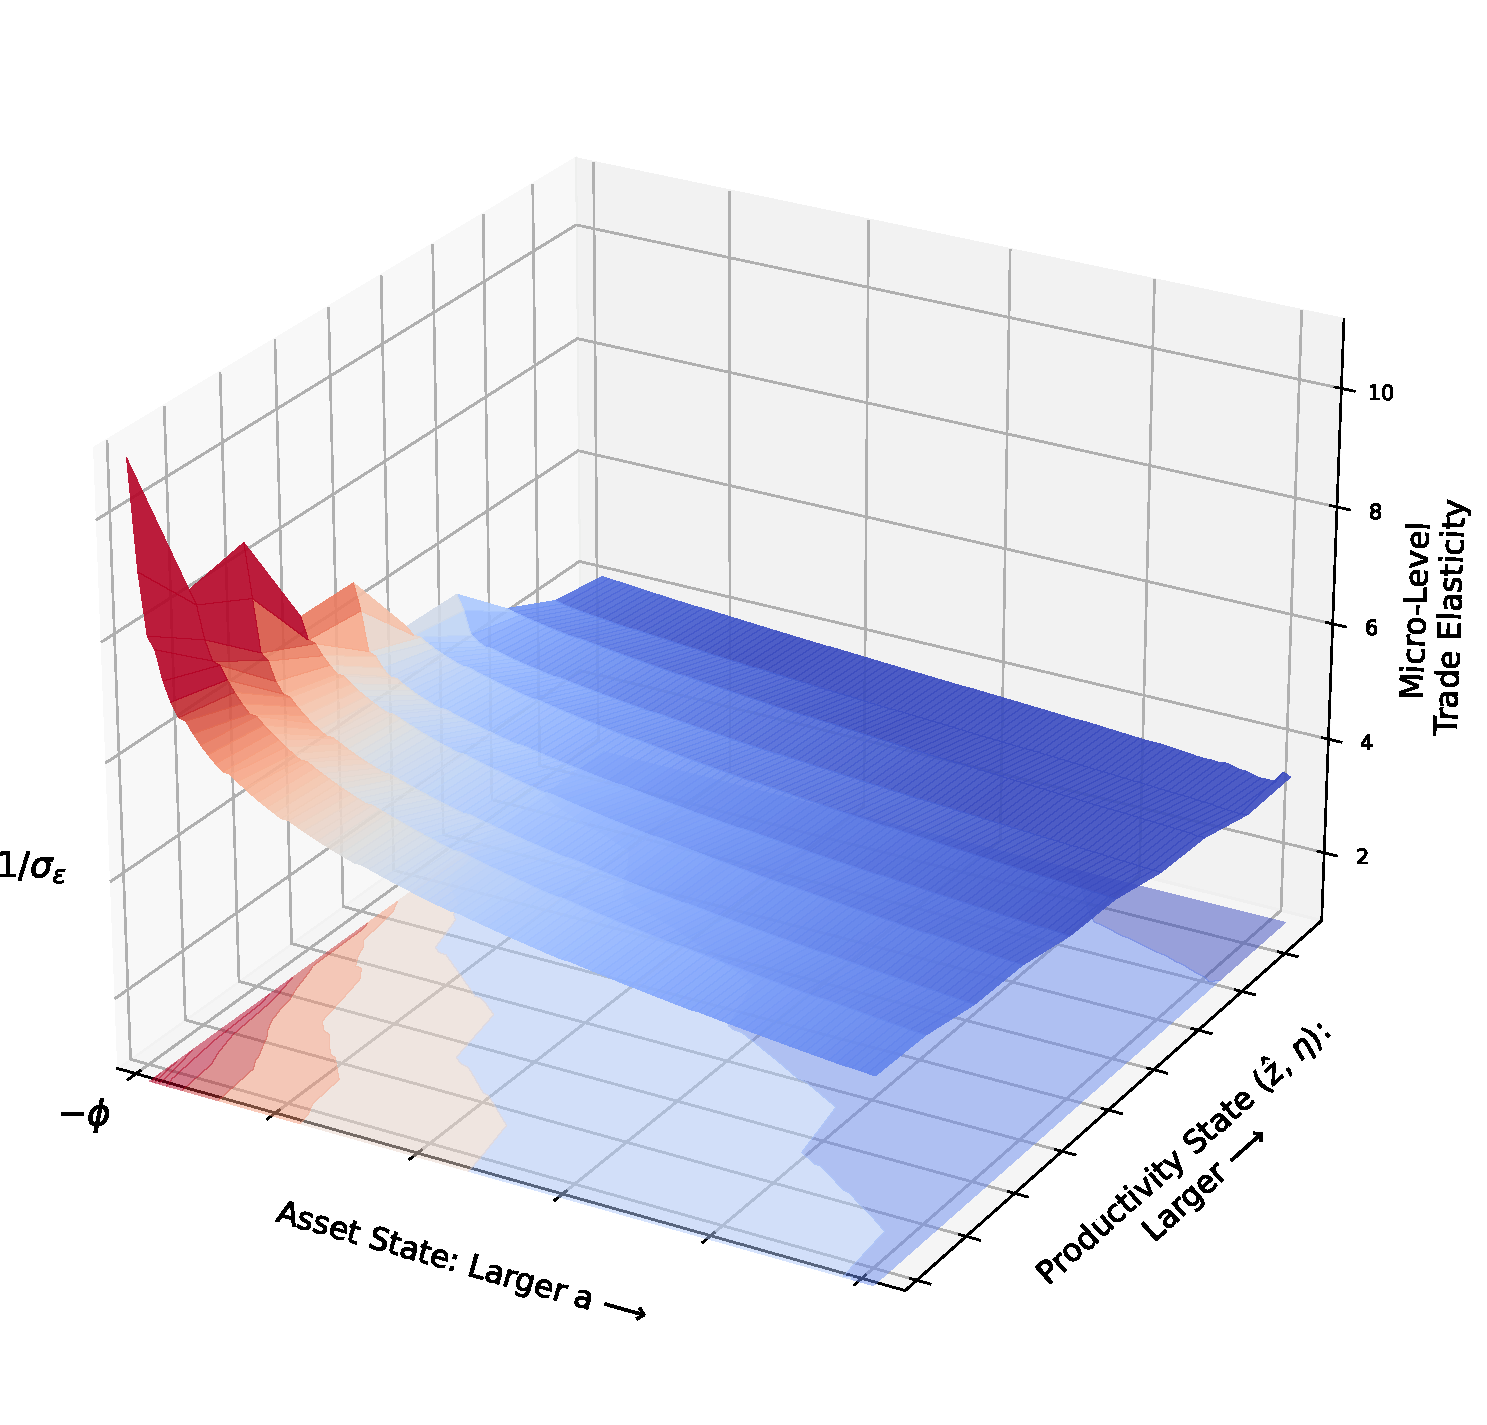
\includegraphics[scale = .37]{./figures/micro-elasticity.pdf}}
\caption{Household-Level Elasticities, $-\theta_{ij}(a,z)$}\label{fig:micro-elasticity}
\end{subfigure}
\begin{subfigure}{.45\textwidth}
\centering
\centering{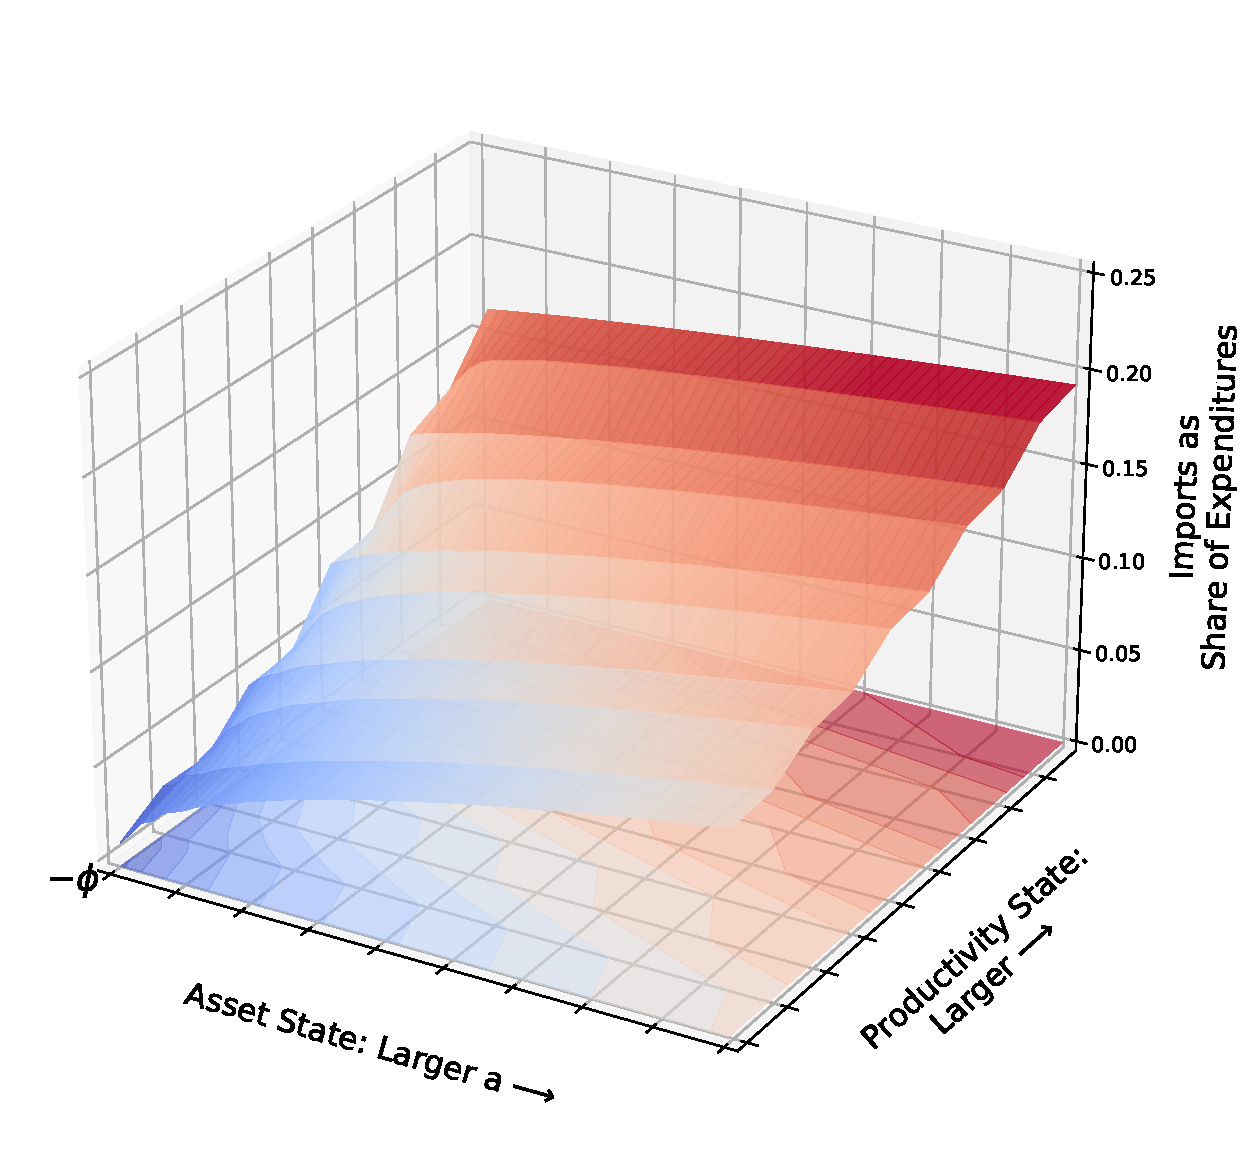
\includegraphics[scale = .37]{./figures/trade-share.pdf}}
\caption{Household-Level Import Shares}\label{fig:micro-trade}
\end{subfigure}
\end{figure}

Figures \ref{fig:micro-elasticity} and \ref{fig:micro-trade} illustrates how this works in a symmetric two country economy. Figure \ref{fig:micro-elasticity} plots the absolute value of the trade elasticity (intensive and extensive margin) by household state (assets are on the x-axis, productivity state on the y-axis), and the borrowing constraint $\phi$ is in the south-west corner. This shows is how the trade elasticity systematically varies with assets and income. Poor households|especially those near the borrowing constraint|are very price elastic, with a trade elasticity of around $-10$. Richer households are less price elastic, with this elasticity declining towards $-3.$

This pattern of elasticities has a strong intuitive feel and there is evidence in support of it.\footnote{This idea goes back to \citeapos{harrod1936trade} ``law of diminishing elasticity of demand'' that says that price sensitivity declines with income. This law is not to be confused with Marshall's second law of demand which I discuss later.}. This result comes out of estimates in \citet{berry1995automobile} and, in a more macro context, \citet{nakamura2010accounting}. \citet{sangani2022markups} is a recent paper that provides evidence in support of this fact from the Kilts-Nielsen data set. The evidence in \citet{auer2022unequal} most closely relates to the patterns in Figure \ref{fig:micro-elasticity} with poorer households having higher price elasticities; \citet{colicev2022impact} finds similar results.

One more implication of this result: because rich and poor households face the same prices, differences in elasticities lead to different expenditure shares. Figure \ref{fig:micro-trade} illustrates this point by plotting expenditure on the foreign good relative to total expenditure. Because of trade costs and symmetry across countries, the home good is the relatively cheaper good. Thus, poor, high-price-elasticity households spend more on the cheap home good than on the expensive foreign good. In fact, for those near the borrowing constraint in this example, expenditure on the imported good is near zero. This pattern appears counterfactual per the evidence of \citet{borusyak2021distributional}, and hence it motivates my introduction of non-price product attributes (quality) in the quantitative application to match micro-level expenditure shares.

\subsection{The Gains from Trade}

In this section I compute how welfare changes due to a change in trade costs. The purpose here is to illustrate mechanics and where the gains from trade arise from. To that end, I derive these gains across steady states where I'm thinking a situation where the change is small and there is an immediate jump to the new steady state.  Unlike the trade elasticity, I take total derivatives that encompass general equilibrium changes in wages and interest rates.

The analysis focuses on how household-level welfare changes. To characterize this, I make the use of the observation in equation (\ref{eq:log_sum-home}) that I can express the ex-ante value function in only in terms of home choice $ii$ values and then recursively push forward. In other words, I can compute the change in the ex-ante value function \emph{as if} the household consumed only the home good for the infinite future.

Appendix \ref{apx-sec:gains-trade} provides the details and leads to the following expression:
{\small
\begin{align}
\frac{\mathrm{d} v_i(a, z)}{\mathrm{d} d_{ij} / d_{ij}} =& \underbrace{-\sigma_{\epsilon} \frac{\mathrm{d} \pi_{ii}(a,z) / \pi_{ii}(a,z)}{\mathrm{d}d_{ij} / d_{ij}}}_{\mathbf{A(a,z)}} \label{eq:welfare-vterms} \\
\nonumber \\
& + \underbrace{u'(c_{i}(a,z,i)) \bigg[ \frac{\mathrm{d} w_{i} / p_{ii}}{\mathrm{d} d_{ij} / d_{ij}}z  +  \frac{\mathrm{d} R_{i} / p_{ii}}{\mathrm{d} d_{ij} / d_{ij}} a  \bigg]}_{\mathbf{B(a,z)}} \nonumber \\
\nonumber \\
& + \underbrace{\bigg \{- \frac{u'(c_{i}(a,z,i))}{p_{ii}} + \beta \mathbb{E}_{z'} \bigg [-\sigma_{\epsilon} \frac{\partial \pi_{ii}(a',z') / \pi_{ii}(a',z')}{\partial a'} + \frac{u'(c_{i}(a',z',i))R_{i}}{p_{ii}} \bigg ] \bigg \}\frac{\mathrm{d} g_{i}(a,z,i)}{\mathrm{d} d_{ij} / d_{ij}}}_{\mathbf{C(a,z)}} \nonumber \\
\nonumber \\
& + \beta \mathbb{E}_{z'} \bigg \{\underbrace{-\sigma_{\epsilon} \frac{\mathrm{d} \pi_{ii}(a',z') / \pi_{ii}(a',z')}{\mathrm{d}d_{ij} / d_{ij}}}_{\mathbf{A(a',z')}} +  \underbrace{u'(c_{i}(a',z',i)) \bigg[ \frac{\mathrm{d} w_{i} / p_{ii}}{\mathrm{d} d_{ij} / d_{ij}}z'  +  \frac{\mathrm{d} R_{i} / p_{ii}}{\mathrm{d} d_{ij} / d_{ij}} a' \bigg]}_{\mathbf{B(a',z')}} \ \  \ldots \nonumber
\end{align}
}Let me walk through the interpretation of each term.


\textbf{Gains from substitution:} The $A(a,z)$ term here is a household-specific gains from substitution term and is summarized by the change in the home choice probability and the dispersion parameter on tastes. The change in the home share summarizes two forces: (i) how exposed a household is to the change through the choice probabilities, and then (ii) elasticities. To see this, define $\bar{\theta}(a,z) ^E_{ij',j}$ as the extensive margin, cross-price elasticity, in total derivative form (and its derivation follows what is done in (\ref{eq:extensive-margin})). As I show in Appendix \ref{apx-sec:gains-trade}, the change in the home share can be expressed as:
\begin{align}
-\sigma_{\epsilon} \frac{\mathrm{d} \pi_{ii}(a,z) / \pi_{ii}(a,z) }{\mathrm{d} d_{ij} / d_{ij}} &= -\sigma_{\epsilon} \sum_{j'} \pi_{ij'}(a,z) \times \bigg[ \bar{\theta}(a,z) ^E_{ii,j} - \bar{\theta}(a,z) ^E_{ij',j}\bigg]. \label{eq:gains-substitution-cross-price}
\end{align}
This says that the change in home choice probability is equivalent to a weighted average of relative cross-price elasticities with the weights being the choice probabilities. The important observation here is that elasticities are showing up and determining the first-order effect from the change in prices. To further clarify things (at the risk of oversimplifying stuff) the next line assumes that all cross-price-elasticity terms are small
\begin{align}
-\sigma_{\epsilon} \frac{\mathrm{d} \pi_{ii}(a,z) / \pi_{ii}(a,z) }{\mathrm{d} d_{ij} / d_{ij}} & \approx
\sigma_{\epsilon} \times \pi_{ij}(a,z) \times \bar{\theta}(a,z) ^E_{ij,j},
\label{eq:gains-substitution}
\end{align}
and then, the gains from substitution depend upon the initial exposure of a household to market $j$ and their own-price elasticity (the total derivative analog to (\ref{eq:extensive-margin})).\footnote{Thinking through (\ref{eq:extensive-margin-large}) and (\ref{eq:gains-substitution}) , one may be tempted (at least I have been) to put (\ref{eq:welfare-vterms}) in money-metric terms by dividing through the marginal utility of consumption as in \citet{walsh2023inflationary} or \citet{moll2022asset}. This approach does not remove the dependence on elasticities because market incompleteness results in marginal utility not being equated across goods choices. In \citet{mongey-waugh-2} we discuss how discrete choice and market incompleteness shapes money metric and equivalent variation welfare measures.} And because the own-price elasticity is intimately connected to marginal utility of consumption per the discussion in Section \ref{sec:trade-elasticity}, the elasticity effect picks up the idea that one aspect of the gains from trade is a household's individual valuation of the price reduction.

This expression connects with two related papers. \citet{borusyak2021distributional} (following an approach dating back to at least \citet{deaton1989rice}) considers an environment where, to a first order, only exposure matters, similar to the exposure term in Equation (\ref{eq:gains-substitution}). \citet{auer2022unequal} work out second order effects with non-homothetic CES preferences, and additional effects from elasticities show up, similarly to the elasticity term in (\ref{eq:gains-substitution}). Here both are present.

\textbf{Gains from factor prices:} The second term $B(a,z)$ captures how a reduction in trade costs affects factor prices | the wage relative to the price of the home good and the interest rate relative to the price of the home good. And these effects are all valued at that household's marginal utility of consumption. I can simplify this term in two ways. First, with perfect competition $\frac{w_i}{p_{ii}} = A_{i}$ from (\ref{eq:marginal-product}), and thus $\frac{\mathrm{d} w_{i} / p_{ii}}{\mathrm{d} d_{ij} / d_{ij}} = 0$, so households are perfectly ``hedged'' from any effect of trade on labor earnings.

The second simplification is that $\frac{\mathrm{d} R_{i} / p_{ii}}{\mathrm{d} d_{ij} / d_{ij}} = \frac{\mathrm{d} R_{i} / w_{i}}{\mathrm{d} d_{ij} / d_{ij}}$, and so the $B(a,z)$ term becomes
\begin{align}
B(a,z) = u'(c_{i}(a,z,i)) \times  a \times \frac{\mathrm{d} R_{i} / w_{i}}{\mathrm{d} d_{ij} / d_{ij}}.
\end{align}
Two issues that this term presents are (i) how does the ratio of the gross interest rate relative to the wage rate change and (ii) how exposed is the household to this change. Unlike labor earnings, households are not perfectly hedged against these changes, and because households can have negative positions in $a$, changes in relative factor prices have distributional effects.  For example, if a trade liberalization leads to an increase in $R / w$, net debtors suffer since their terms to borrow deteriorate, while net savers benefit. Broadly speaking this force is very much analogous to textbook discussions about how unexpected inflation leads to redistribution between borrowers and lenders and specifically it is closely related to the points made in \citet{auclert2019monetary} and \citet{moll2022asset}.


\textbf{Gains from changes in asset holdings:} The third term, which I'm labeling as $C(a,z)$, is about changes in asset holdings. For the small / local changes that I'm considering it should zero out, but for larger changes, this term could be relevant. Let me expand upon this.

First, notice that the inside the bracket term is the Euler equation from (\ref{eq:euler_equation-home}), and it's multiplied by the change in policy function. Now, if the household is unconstrained, the inside-the-bracket term is zero, as there is no gain through changes in asset behavior. Asset holdings are already chosen optimally so that margins are equated; thus, any benefit of lower trade costs on changes in asset behavior is zero. This inside-the-bracket term may not be zero, because of borrowing-constrained households. However, the bracket is multiplied by the change in the asset policy function. Now if the household is constrained, then assets can't adjust. So the outside term is zero and thus overall the $C(a,z)$ term is zero. Via this logic, the only people that benefit (and contribute to social welfare) through changes in asset holding are those on the margin between constrained and not-constrained. But if they are on the margin between being constrained and not-constrained, then they are on their Euler equation anyways.

\textbf{Future Gains:} Finally, these terms repeat themselves into the expected future, appropriately discounted. This last point | that today and the future matters | suggest that my discussion above oversimplifies things. In this model, the poor today are rich in the future; and the rich today are poor in the future. These dynamics work to make the gains \emph{more equal}. For example, if the gains from trade are biased towards the poor, the rich today gain because being poor is not as bad as it used to be.

Proposition \ref{prp:gains-trade} summarizes the result below.

\begin{prp}[\textbf{HA Gains from Trade}] \label{prp:gains-trade} Household level gains from trade are given by
{\footnotesize
\begin{align}
\nonumber
\frac{\mathrm{d} v_i(a, z)}{\mathrm{d} d_{ij} / d_{ij}} = \mathbb{E}_{z} \sum_{t = 0}^{\infty} \beta^{t} \bigg \{ A(a_{t},z_{t}) + B(a_{t},z_{t}) + C(a_{t},z_{t}) \bigg \}
\end{align}
}where each term represents:
\begin{itemize}
\item gains from substitution: $A(a_{t},z_{t}) = -\sigma_{\epsilon} \frac{\mathrm{d} \pi_{ii}(a_{t},z_{t}) / \pi_{ii}(a_{t},z_{t})}{\mathrm{d}d_{ij} / d_{ij}}$;

\item gains from factor prices: $B(a_{t},z_{t}) = u'(c_{i}(a_{t},z_{t},i))\frac{\mathrm{d} R_{i}/p_{ii}}{\mathrm{d} d_{ij} / d_{ij}}a_{t}$;

\item gains from changes in asset holdings:
{\footnotesize
\begin{align}
\nonumber
C(a_{t},z_{t}) = \bigg \{- \frac{u'(c_{i}(a,z,i))}{p_{ii}} + \beta \mathbb{E}_{z'} \bigg [-\sigma_{\epsilon} \frac{\partial \pi_{ii}(a',z') / \pi_{ii}(a',z')}{\partial a'} + \frac{u'(c_{i}(a',z',i))R_{i}}{p_{ii}} \bigg ] \bigg \}\frac{\mathrm{d} g_{i}(a,z,i)}{\mathrm{d} d_{ij} / d_{ij}},
\end{align}}
which is zero for small changes.
\end{itemize}
\end{prp}

\subsection{Elasticities and Gains in the Efficient Allocation}\label{sec:efficient}

One issue behind the results above is market incompleteness. Households are imperfectly insured against the risks they face, which leads to heterogeneity in the marginal utility of consumption and, in turn, heterogeneity in price sensitivity, expenditure patterns, and the gains from trade. Building on work in from my paper (\citet{waughoptimal}), I contrast the previous results (Propositions \ref{prp:GET} and \ref{prp:gains-trade}) with the elasticities and gains from trade in an allocation where a social planner can overcome market incompleteness. Appendix \ref{apx-sec:efficient} provides a self-contained discussion of the planning problem and derivation of the results.

The starting point is a utilitarian social welfare function and the Planner chooses consumption allocations $c_{i}(z, j, t)$ and choice probabilities $\pi_{ij}(z,t)$ for all $i,j$ pairs, $z$ states, and dates $t$ to maximize social welfare.\footnote{In a more general, but static setting, \citet{mongey-waugh-2} characterize complete markets and efficient allocations in discrete choice models. \citeapos{lagakos2023welfare} model of migration is an important precursor to my characterization of the gains from trade under efficiency here.} Given a characterization of the optimal allocation, I can compute trade elasticities and the welfare gains from a change in trade costs and study how welfare changes across the two stationary allocations.\footnote{In contrast to the previous section, the move across stationary allocations is of no consequence as there is no moving aggregate state variable, so the jump across stationary equilibrium is instantaneous.}

Proposition \ref{prp:gains-efficient-allocation} describes the result; Appendix \ref{apx-sec:efficient} works out the details.

\begin{prp}[\textbf{Trade Elasticities and Welfare Gains in the Efficient Allocation}]\label{prp:gains-efficient-allocation} The elasticity of trade to a change in trade costs between $ij$ in the efficient allocation is:
\begin{align}
\theta_{ij} =  -\frac{1}{\sigma_{\epsilon}} \bigg [ u'(c_{i}(j)) c_{i}(j) \bigg]. \label{eq:eff-trade-elasticity}
\end{align}
And the welfare gains from a reduction in trade costs between $i,j$ are
\begin{align}
\frac{\mathrm{d} W }{\mathrm{d} d_{ij} / d_{ij}} &= \frac{\sigma_{\epsilon} \  \theta_{ij} \  \pi_{ij} \ L_i}{1-\beta},
\label{eq:eff-trade-gains}
\end{align}
which is the discounted, direct effect from relaxing the aggregate resource constraint. And this can be expressed as
\begin{align}
= -\sigma_{\epsilon} \times \frac{\mathrm{d} \pi_{ii} / \pi_{ii}}{\mathrm{d} d_{ij} / d_{ij}} \times \frac{L_i}{1 - \beta}.
\label{eq:eff-trade-gains-acr}
\end{align}
\end{prp}
Proposition \ref{prp:gains-efficient-allocation} highlights a couple of things. Very similar to the household-level extensive margin elasticity in (\ref{eq:extensive-margin-large}), the aggregate trade elasticity has a term with the marginal utility of consumption times consumption showing up. Like in the discussion above, this term matters for the elasticity in a very intuitive way|country pairs that deliver a lot of utility, on the margin, are the pairs where the planner will be most responsive to changes in trade costs. In contrast to the decentralized allocation, households' private valuations align with social valuations, and so heterogeneity is irrelevant for the elasticity of trade.

The second part of Proposition \ref{prp:gains-efficient-allocation} summarizes the gains from trade. It says that the total change in welfare is the share of households consuming commodity $j$ times the number of households in country $i$. In other words, the number of households eating that commodity. This is then converted into utils using the elasticity, which as discussed above, involves the dispersion in shocks and then the rate at which utils are being delivered at current quantities.\footnote{An alternative perspective is to divide through both sides of (\ref{eq:eff-trade-gains}) by the marginal utility of consumption. Then, welfare is in money metric units.} This is then discounted for the infinite future, hence the $1/ (1-\beta)$ term.

This is just the direct effect from a reduction in trade costs relaxing the resource constraint and converted to utils appropriately. Behind this result is an envelope-type argument in which direct effects matter only because I'm evaluating the change in welfare at the optimized allocation and any benefits of adjusting consumption and choice probabilities are zero|on the margin.

This result is reminiscent of \citet{AtkesonBurstein2010}, who make a similar claim in the context of a model with rich firm heterogeneity. They show that the only first order effect of lower trade costs on welfare is the direct consumption effect. My result is similar, but with household heterogeneity. It says that in the efficient allocation household heterogeneity becomes irrelevant and the welfare gains from trade only about the savings from

The final part of Proposition \ref{prp:gains-efficient-allocation} connects with \citet{arkolakis2012new}. As I show in the Appendix, in the efficient allocation, the percent change in the home choice probability exactly equals the $ij$ choice probability times the trade elasticity:
\begin{align}
\frac{\mathrm{d} \pi_{ii} / \pi_{ii}}{\mathrm{d} d_{ij} / d_{ij}} = -\theta_{ij} \times \pi_{ij}.
\label{eq:effecient-home-share}
\end{align}
Then inserting (\ref{eq:effecient-home-share}) into  (\ref{eq:eff-trade-gains}) delivers the final line of Proposition \ref{prp:gains-efficient-allocation}. Now, the form of (\ref{eq:eff-trade-gains}) is closely related to \citet{arkolakis2012new}. Interestingly, and similar to the decentralized allocation, the change in the home choice probability summarizes a lot. Moreover, now there is an equivalence between \citet{AtkesonBurstein2010}-like logic and \citet{arkolakis2012new}-style formulas.

There are two details: choice probabilities do not necessarily correspond to expenditure shares, and the $\sigma_{\epsilon}$ is not the inverse of the trade elasticity. However, with $\log$ preference the trade elasticity becomes $1 / \sigma_{\epsilon}$, choice probabilities are proportional to expenditure shares, and the correspondence between the gains from trade under efficiency and \citet{arkolakis2012new} becomes exact. The case of $\log$ has many other implications in the decentralized allocation. I turn to this case next.

\subsection{The Case of $\log$ Preferences}\label{sec:log-preferences}

The case of $\log$ preferences over the physical commodity displays some unique features. This (very common) preference structure leads to an interesting result where micro-level heterogeneity and market incompleteness completely separate from the trade side of the economy. So in this one case, trade behaves ``as if'' there were a representative agent Armington-CES consumer.

Consider the following preference structure:
\begin{align}
\tilde{u}( c_{ij,t} ) =  \log(c_{ij,t}) + \epsilon_{j,t}. \nonumber
\end{align}
There is essentially one insight, and then everything follows. Examining the problem in (\ref{eq:value_fun_option}) and substituting in the households, budget constraint from (\ref{eq:trade-budget-constraint}), the observation is that the optimal $a'$ conditional on a choice $j$ is \textbf{independent} of the choice $j$. And this observation implies that choice probabilities become independent of states $a$ and $z$. Everything follows from these observations, and Proposition \ref{prp:GET} and Proposition \ref{prp:gains-trade} can be applied. Corollary \ref{prp:seperation} states the result and Appendix \ref{apx-sec:log-preferences} works through this logic step-by-step.

\begin{corr}[\textbf{Separation of Trade and Heterogeneity}]\label{prp:seperation} In the dynamic, heterogeneous agent trade model where preferences are logarithmic over the physical commodity, the trade elasticity is
\begin{align}
\theta = -\frac{1}{\sigma_{\epsilon}}, \nonumber
\end{align}
and trade flows satisfy a standard gravity relationship:
\begin{align}
\frac{\pi_{ij}}{\pi_{ii}} = \frac{M_{ij}}{M_{ii}} = \left( \frac{  w_{j} / A_{j} }{  w_{i} / A_{i} } \right)^{\frac{-1}{\sigma_{\epsilon}}} d_{ij}^{\frac{-1}{\sigma_{\epsilon}}}. \nonumber
\end{align}
The welfare gains from trade for an individual household are
\begin{align}
\nonumber
\frac{\mathrm{d} v_i(a, z)}{\mathrm{d} d_{ij} / d_{ij}} = \underbrace{\frac{1}{\theta (1-\beta)} \times \frac{\mathrm{d} \pi_{ii} / \pi_{ii}}{\mathrm{d}d_{ij} / d_{ij}}}_{A} \ \ + \ \
\mathbb{E}_{z} \sum_{t = 0}^{\infty} \beta^{t} \bigg \{ B(a_{t},z_{t}) + C(a_{t},z_{t}) \bigg \},
\end{align}
where the gains from substitution are (i) independent of the household heterogeneity and (ii) summarized by the trade elasticity and the change in the home expenditure share. The other sources of gains are as in Proposition \ref{prp:gains-trade}.
\end{corr}
The first part of this result shows heterogeneity plays no role in determining the aggregate trade elasticity. As in the CES-Armington model or \citet{eaton2002technology}, it's just about how innately substitutable national varieties are. The next part of this result says that the ratio of choice probabilities are equal to the ratio of trade flows (again like in \citet{eaton2002technology}) and that aggregate trade satisfies a gravity relationship with no role for household heterogeneity.

The first part of the welfare formula connects with seminal results. Because choice probabilities are independent of states (and proportional to expenditure shares), applying Proposition \ref{prp:gains-trade} says that the gains from substitution term (my $A$-term) becomes independent of household heterogeneity. And other than discounting, this is analogous to the result in \citet{arkolakis2012new}.

One can go a step further and show that substitution does not play a role, but this term just reflects the direct effect of changes in the terms of trade. To see this, note that the change in the home share equals
\begin{align}
\frac{1}{\theta} \frac{\mathrm{d} \pi_{ii} / \pi_{ii}}{\mathrm{d}d_{ij} / d_{ij}} = \sum_{j'} \pi_{ij'} \bigg \{  \frac{\mathrm{d} p_{ij'} / p_{ij'}}{\mathrm{d}d_{ij} / d_{ij}} - \frac{\mathrm{d} p_{ii} / p_{ii}}{\mathrm{d}d_{ij} / d_{ij}} \bigg \},
\end{align}
where the right-hand side is the expenditure-weighted change in relative prices. This formula is exactly analogous to \citet{deaton1989rice}-style formulas where expenditure shares are sufficient statistics to evaluate the effects price changes. And what makes this possible, unlike equation (\ref{eq:gains-substitution-cross-price}), is that elasticities do not show up. It's just about shares $\times$ relative price changes so substitution effects are \emph{not} first-order here.

Finally, and unlike the $A$ component of my welfare formal, the second component as to how changes in factor prices influence welfare remains heterogenous. This is the one place where incomplete markets matters.

To be honest, I found these results surprising. By looking at the choice probabilities in (\ref{eq:choice-prob}) and noting how the value functions determine choices, not period utility functions, one would suspect that the households' income fluctuations problem would shape aggregate trade outcomes. Corollary \ref{prp:seperation} shows that is not the case but that micro-outcomes and aggregate trade outcomes ``separate.''

Proposition \ref{prp:seperation} is also interesting because it generalizes the results of \citet{anderson1987ces} and \citet{anderson1992discrete} to a far more complicated economy. They showed that in a static model with log utility and additive logit shocks, the economy behaves \emph{as if} there were a representative agent CES consumer. I recover their result, but I must emphasize the complexity of the economy at the micro-level for which this result stands|households are forward looking, face productivity and taste shocks in the presence of incomplete markets, and borrowing constraints. Yet, these details don't matter when the magic of $\log$ kicks in.

\section{Calibration}

This section focuses on my approach to calibrating the model. The next two subsections discuss the preference specification, income and taste shock process, borrowing constraints, and my method of scaling things so the model can deliver balanced growth-like properties.

The final section follows the trade literature by picking country-specific TFP and trade cost parameters to match bilateral trade flows. How I do this is an indirect inference procedure | ``gravity as a guide'' | to overcome the fact that my model does not admit a closed form map from trade flows to parameters, as static, gravity models do. I describe this approach below.

\subsection{Preferences, Shocks, and Constraints}

Table \ref{tb-calibration} provides an overview of the non-country-specific parameters (or if they are country specific, they are all scaled in the same way). Below, I discuss each choice in turn.

Utility over the physical commodity is CRRA with relative risk aversion $\gamma$. This parameter is calibrated (along with the taste shock parameter) to match the price elasticities of the median ( -4.4 ) and poor households ( -6.6 )  in the data of \citet{auer2022unequal}. And the correspondence between this parameter and these moments is motivated by the results in (\ref{eq:extensive-margin-large}) and (\ref{eq:elasticity-mpc}) showing how the curvature of the utility function partially shapes micro-level elasticities and how they vary across households.

In addition to these choices, I do two things to ensure that micro and macro facts can be matched.

The first feature I introduce is household-specific quality shifters. Mechanically, I implement quality shifters by introducing a home bias term $\psi_{i}(z,i)$, which additively shifts period utility when consuming the home good $i$ and differs by the household's productivity state $z$. Appendix \ref{apx-sec:quality} provides details, but the key issue is that with the additivity, it affects only choice probabilities, not elasticities per se. To reduce $\psi$s dimensionality, I assume that it's a log-linear function of a household's permanent productivity state and this function is the same across countries. The slope of this relationship is calibrated to match the fact from \citet{borusyak2021distributional} that import expenditure shares are essentially the same between US poor (below median income) and rich (above median income) households. And as equation (\ref{eq:gains-substitution}) motivates, how import shares vary across rich and poor households is an important input into determining how the gains from trade vary across households.

The necessity of quality shifters relates to the discussion around Figure \ref{fig:micro-trade} | that only prices and price elasticities determine how shares vary across households. And these forces lead to a pattern of sorting with poor, high-elasticity households concentrating their expenditures on the cheapest commodities available. Quality shifters that vary with household-specific characteristics are one way to match shares, yet allow for heterogeneity in price elasticities. \citet{berry1995automobile} make this point, and it motivates their modeling of demand with interactions between attributes of the product and household characteristics; \citet{auer2022unequal} allows for this force as well in both their model and empirical specification.

The second feature I want is that things scale and deliver balanced growth-like behavior. Specifically, the want-operator here is that if there are two countries one with high TFP and one with low TFP but otherwise identical, elasticities (at the micro and macro level) in the two countries are the same. The way to do this is to make the Type 1 extreme value parameter country specific and scaled so that $\sigma_{\epsilon,i} = \sigma_{\epsilon} A_i^{1-\gamma}$ and similarly for the quality shifters above. The common component of the taste shock parameter, $\sigma_{\epsilon}$ is calibrated to match the price elasticities of the median and poor households in the data of \citet{auer2022unequal}.

The income shock process is set up to be a mixture of a AR(1) persistent component and an iid transitory component, and this is calibrated using results from \citet{krueger2016macroeconomics}. I use their exact parameter values at an annual frequency. It is the same across countries.

The borrowing constraint is set in the following way. I scale it by a country's autarky level of average real labor income. Then, the borrowing constraint is set so that a household can borrow up to 50 percent of its autarky level of income. The scaling here is done (again) to deliver a balanced-growth-like property of the model so a households debt capacity is invariant to a country's autarky level of income. The precise number of 50 percent seems reasonable to me, but as a check, I show that the marginal propensities to consume and how they vary across households are consistent with the evidence of \citet{kaplan2022marginal}.

\begin{table}[t]
\small
\begin{center}
\refstepcounter{table}
\setlength {\tabcolsep}{4.5mm}
\renewcommand{\arraystretch}{1.60}\label{tb-calibration}
\begin{tabular}[t]{l c l}
\multicolumn{3}{c}{{\normalsize\textbf{Table \ref{tb-calibration}: Preferences, Shocks, and Constraints | Calibrated Parameters}} }
\\\hline \hline
Description & Value & \multicolumn{1}{c}{Target}\\
\cmidrule(lr){1-1} \cmidrule(lr){2-2} \cmidrule(lr){3-3}
Discount Factor, \ $\beta$                          & $0.92$ & \phantom{\} } Global Interest Rate of $1\%$ \\
CRRA parameter, \ $\gamma$                          & $1.45$ & \multirow{2}{*}{\Bigg \} Micro elasticities of {\small \citet{auer2022unequal}} }\\
Type One E-V parameter, \ $1 / \sigma_{\epsilon}$    & $3.0\phantom{0}$ & \\
Slope of Quality Shifter, \ $\psi_{ii}(z)$          & $0.72$ & \phantom{\} } Micro moments of {\small \citet{borusyak2021distributional} } \\
Borrowing Constraint \ $\phi_{i}$                   & --- & \phantom{\} } $50\%$ of $i$'s autarky labor income \\
Income Process on \ $z$                             & --- & \phantom{\} } {\small \citet*{krueger2016macroeconomics}} \\
\hline
\end{tabular}
\\[0.5ex]
%\parbox{5.95in}{\footnotesize \textbf{Note:} }
\end{center}
\end{table}

All the quantitative results I show are for the case of financial globalization. In this case there is one interest rate clearing the global asset market. Households in all countries have the same discount factor, and I calibrate the discount factor so the equilibrium world interest rate is 1 percent.

\subsection{Using Gravity As a Guide to Match Bilateral Trade Data}

In analyzing how changes in trade frictions affect outcomes, I want the model to match the spatial distribution of economic activity in the data. The calibration challenge is that the model does not admit a gravity representation that allows researchers to invert trade frictions and productivity levels from trade flows, as in \citet{eaton2002technology} and many subsequent papers. Similarly, the model does not admit the use of exact-hat algebra, which allows the research to construct counterfactuals without the knowledge of primitives like trade frictions or productivity (see, e.g., \citet{costinot2014trade} or the dynamic extension in \citet{caliendo2015trade}).

My calibration strategy is to use the gravity regression as a guide in an indirect inference procedure where I estimate parameters of the model so that the regression coefficients from a standard gravity regression run on my model's data match the coefficients when the same regression is ran on the data. Here are the details.

The bilateral trade flow data that I use are from \citet{eaton2002technology}. The data set comprises 19 countries, so it is a nice size to do what I want to do in about an afternoon. In the 19 country model, the parameters I need to choose are $19 - 1$ country-specific TFP parameters (the $A_i$s with the minus because one normalization is free) and then $(19-1) \times (19-1)$ trade costs (with the minus one since the $ii$ trade costs are normalized to one) to infer. This leaves me under-identified with  only $(19-1) \times (19-1)$ bilateral trade shares and $19 -1$ TFP parameters.

\textbf{Step 0.} I reduce the number of parameters to estimate by placing a restriction on trade costs such that they are a function of observable data. Specifically, I assume that trade costs take the form
\begin{align}
\log d_{ij} = d_{k} + b + l + e_{h} + m_{i},
\label{eq:trade-cost-function}
\end{align}
as in \citet{eaton2002technology}, where trade costs are a logarithmic function of distance, where $d_k$ with $k = 1,2,...,6$, is the effect of distance between country $i$ and $j$ lying in the $k$-th distance interval.\footnote{Intervals are in miles: $[0,375)$; $[375,750)$; $[750,1500)$; $[1500,3000)$; $[3000,6000)$; and $[6000,\mbox{maximum}]$. } The $b$ term is the effect of a shared border; $b =1$ if countries $i$ and $j$ share a border and zero otherwise. Similarly $l$ is a dummy variable if countries $i$ and $j$ share a language, and $e_{h}$ represent two dummy variables for different indicators of European integration. The final part is an importer fixed effect that shifts trade costs up or down, depending upon the identity of the importer.

At this point, I've reduced the parameter space to the  coefficients on the trade cost function rather than the complete matrix of trade costs and then the TFP terms.

\textbf{Step 1.} The next step is to run the following gravity regression on the data:
\begin{align}
\log \left( {\frac{M_{ij}}{M_{ii}}} \right) = {im_{i}} + {ex_{j}} + {d_{k}} + {b} + {l} + {e_{h}} + \delta_{ij},
\label{eq:gravity-data}
\end{align}
which projects imports between country $i$ and $j$ ( normalized relative to domestic expenditures ) on an importer effect, exporter effect, and then the gravity variables relating to distance, border, language, and so on. Finally, there is an error term $\delta_{ij}$ reflecting other factors not in this specification.

This is the canonical representation of trade flows | the gravity model. In models along the lines of Armington-CES, \citet{eaton2002technology}, or \citet{melitz2003impact} style model, the importer effects and exporter effects have specific interpretations. And given the point estimates from (\ref{eq:gravity-data}), productivity and the importer fixed effects on the trade cost function are easily recovered. In my model, this is not the case. However, the idea is to use the point estimates from (\ref{eq:gravity-data}) as moments for my model to match. The next step constructs model analogs to (\ref{eq:gravity-data}).

\textbf{Step 2.} To construct model analogs to (\ref{eq:gravity-data}), I guess TFP parameters and coefficients on the trade cost function in (\ref{eq:trade-cost-function}). Define this parameter vector as $\Theta$.

Given $\Theta$, I compute an equilibrium of the world economy. This amounts to: (i) solving for households' dynamic problems in each country, (ii) constructing the stationary distribution of wealth and expenditure patterns in each country, (iii) aggregating, and then (iv) finding a vector of prices so goods markets and financial markets clear worldwide.

Once I find an equilibrium, I run the same regression as in (\ref{eq:gravity-data}) on the model generated data.\footnote{One approach, that works well with good guesses and takes about an hour (rather than 6-12) is to have the solver simultaneously look for prices that clear markets \emph{and} coefficients such that the trade moments are matched.} As a note on notation, the model constructed moments are defined as, for example, $im_{i}(\Theta)$, which is the importer effect estimated on model generated data under the parameter vector $\Theta$.

\textbf{Step 3.} The final step constructs moment conditions, which provide the foundation for estimation / calibration. Define $\mathbf{y}(\Theta)$ as a set of moment conditions comparing the point estimates from the data with the point estimates from the model under the parameter vector $\Theta$. For example, ${im_{i}} - im_{i}(\Theta)$.

My estimation procedure is based on the moment condition
\begin{align}
E\left[\mathbf{y}(\Theta_o)\right] = 0,
\end{align}
where $\Theta_o$ is the true value of $\Theta$. Thus, my method of moments estimator is
\begin{align}
\hat{\Theta} = \arg\min_{\Theta} \left[\mathbf{y}(\Theta)'\ \mathbf{y}(\Theta)\right]. \label{eq:smm-condition}
\end{align}
At a mechanical level, finding the minimum to (\ref{eq:smm-condition}) amounts to returning to \textbf{step 2} each time and smartly updating parameter guess for $\Theta$. One of the nice features of this set-up and the dimensionality reduction that I did is that now this is an exactly identified problem and standard root-finding techniques can be applied to update $\Theta$ and a minimum found.

\subsection{Calibration Results}

\textbf{Shares, Elasticities, and MPCs.} The second column of Table \ref{tb-calibration} reports the calibrated parameters associated with preferences, shocks and constraints. The resulting parameter values for preferences are very plausible. The risk-aversion parameter is 1.45, seemingly not far from $\log$, and well within standard benchmarks in the macro-literature. The Type 1 extreme value parameter is 3.0, which is plausible in the sense that in the $\log$ model this value implies a trade elasticity of 3.0. This is low, but in the range of estimated aggregate trade elasticities.

Figure \ref{fig:quant-micro-elasticity} reports the resulting elasticities and how they vary across the distribution of expenditure for US households in the model. These are right in the ballpark of \citet{auer2022unequal}. If anything, they slightly understate the heterogeneity in elasticities, with rich households being more elastic in my model.

Figure \ref{fig:quant-shares} reports how household-level import expenditure shares vary across the income distribution. The calibration target was such that the share of imports out of total expenditure for households below median income is the same as those above the median. This was met. However, there is some slight non-monotonicity, with households in the middle of the distribution being slightly more exposed to trade than those at the tails of the distribution. This non-monotonicity is associated with the imperfect correlation between income and asset holdings and the fact that quality shifters work only though income. Overall, the pattern is consistent with the facts found in \citet{borusyak2021distributional}. If there is any bias, it is for poor households to experience \emph{fewer} gains from trade as they are slightly less exposed relative to the median household.

\begin{figure}[t!]
\centering
\caption{Household-Level Outcomes}
\begin{subfigure}{.48\textwidth}
\centering
\centering{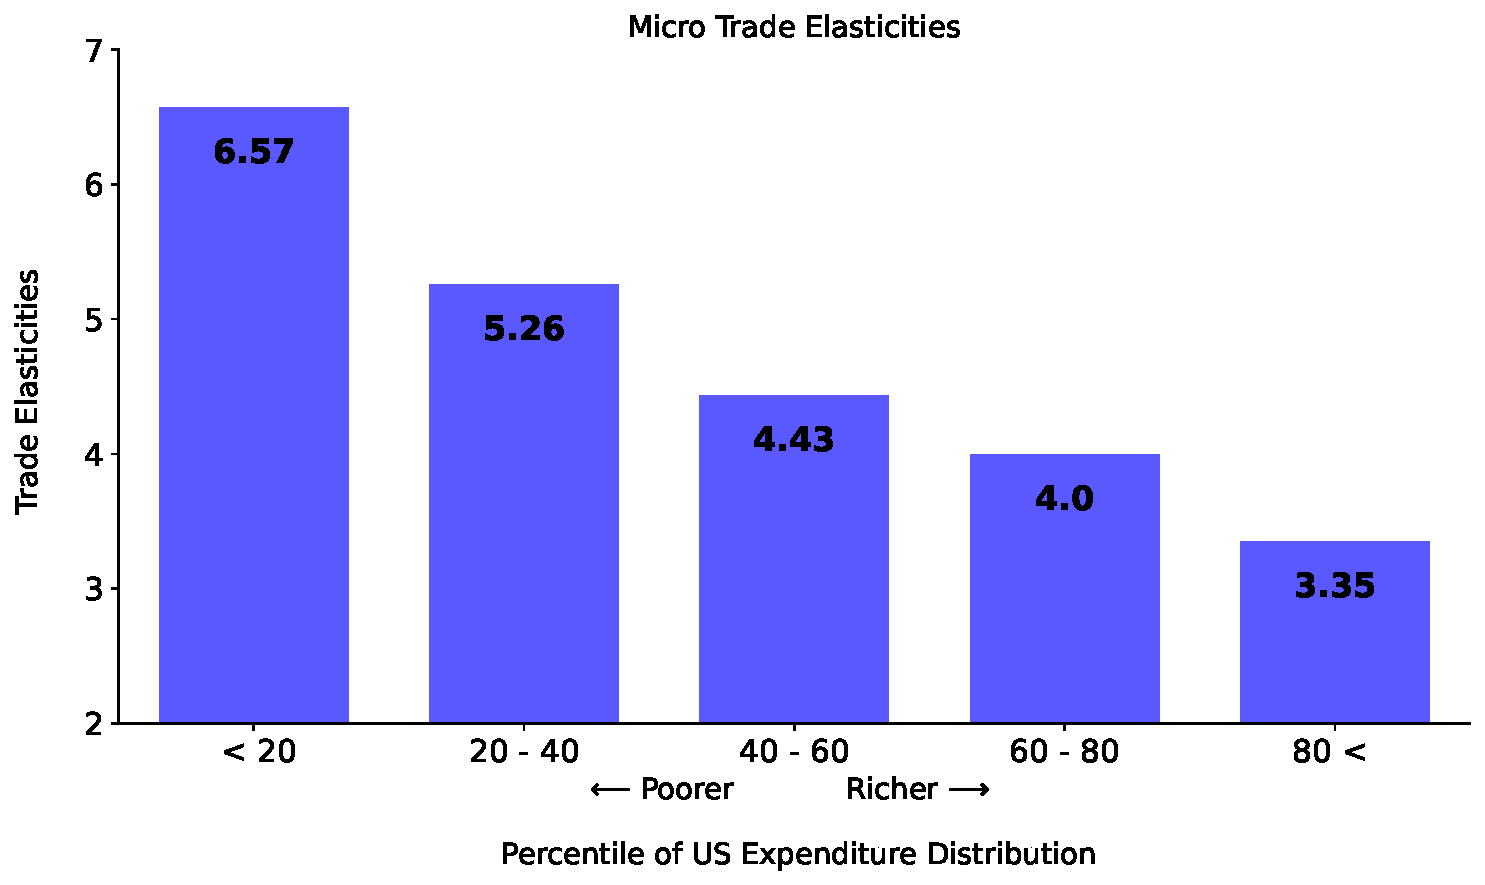
\includegraphics[scale = .3]{./figures/elasticity-micro.pdf}}
\caption{Household-Level Trade Elasticities}\label{fig:quant-micro-elasticity}
\end{subfigure}
\begin{subfigure}{.48\textwidth}
\centering
\centering{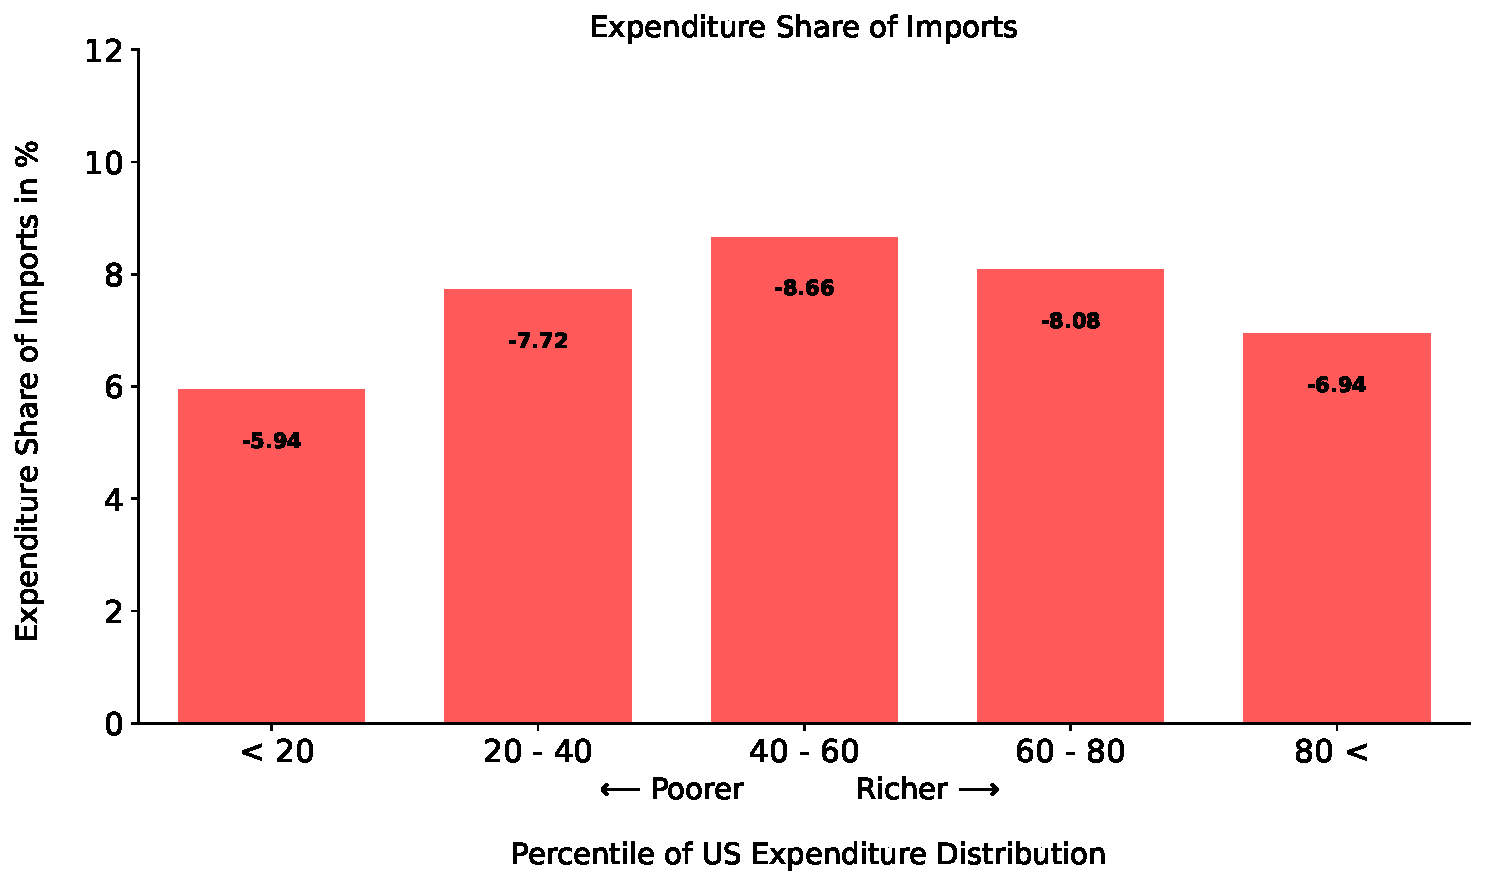
\includegraphics[scale = .3]{./figures/expenditure-share.pdf}}
\caption{Household-Level Import Expenditure Shares}\label{fig:quant-shares}
\end{subfigure}\\
\bigskip
\begin{subfigure}{.758\textwidth}
\centering
\centering{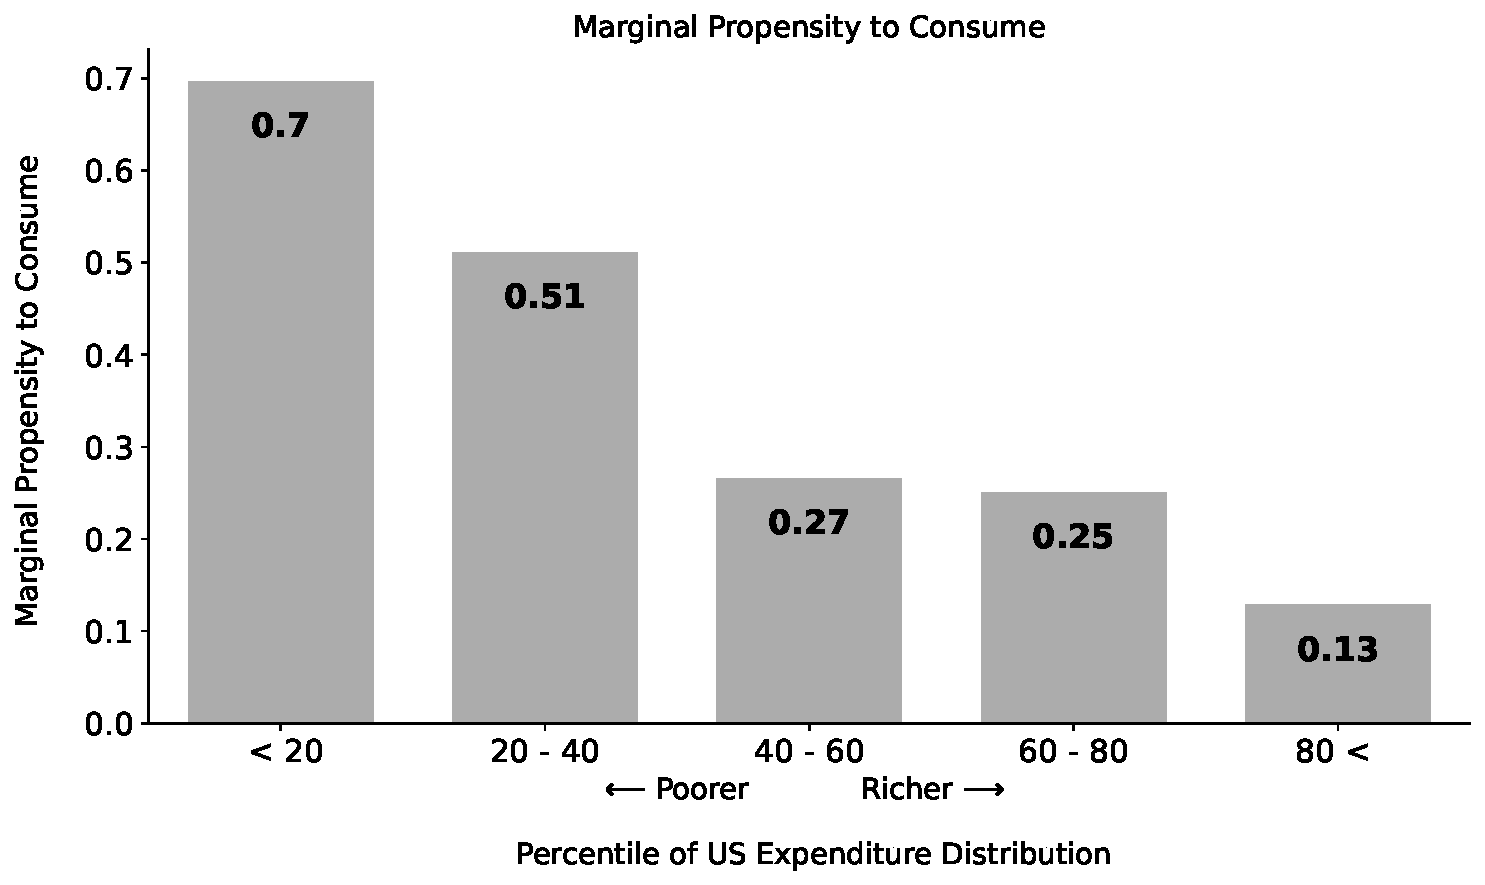
\includegraphics[scale = .3]{./figures/mpc.pdf}}
\caption{Household-Level Marginal Propensities to Consume}\label{fig:quant-mpcs}
\end{subfigure}
\end{figure}


As discussed in Section \ref{sec:trade-elasticity}, how trade elasticities vary across households relates to how marginal propensities to consume (MPC) vary across households (see equation (\ref{eq:elasticity-mpc})). I check the plausibility of the MPCs in my model by endowing households with a one time, unanticipated cash transfer of 1,000 USD and then compute how consumption changes relative to the transfer. As with the elasticities, household level MPCs are aggregated across the different consumption baskets by the household's expenditure weights.

Figure \ref{fig:quant-mpcs} shows that MPCs are right in the ballpark of what is typically thought plausible with the median annual MPC being a little under 0.30, implying that the median household spends about 30 cents per dollar of transfer on consumption; poorer households have substantially higher MPCs and richer households lower. All of these results are consistent with the evidence discussed in \citet{kaplan2022marginal}.\footnote{With that said, this calibration achieves high MPCs essentially by having little wealth in the economy. This feature is consistent with the small quantity of liquid wealth observed in the US economy, but abstracts from large amounts of illiquid wealth.} Together with Figure \ref{fig:quant-micro-elasticity}, one sees the relationship between how sensitive a household is to prices and how sensitive a household is to cash transfers.

To summarize, the model is quantitatively the following salient facts (i) poor households' higher price elasticities relative to rich households, as shown in \citet{auer2022unequal}, (ii) similar import expenditure shares between rich and poor households, as shown in \citet{borusyak2021distributional}, and (iii) patterns of marginal propensities to consume as surveyed in \citet{kaplan2022marginal}.


\textbf{Aggregate Trade and Trade Elasticities.} Figure \ref{fig:model-fit} provides a sense of model fit with respect to bilateral trade flows. The y-axis reports bilateral trade data. and the x-axis reports the outcome from my model. The fit is very high, and nearly indistinguishable from, for example, how a standard trade model would perform. The same is true $\log$ preference model, which, per Proposition \ref{prp:seperation}, should (and does) operate just like a standard trade model.

\begin{figure}[!t]
\centering{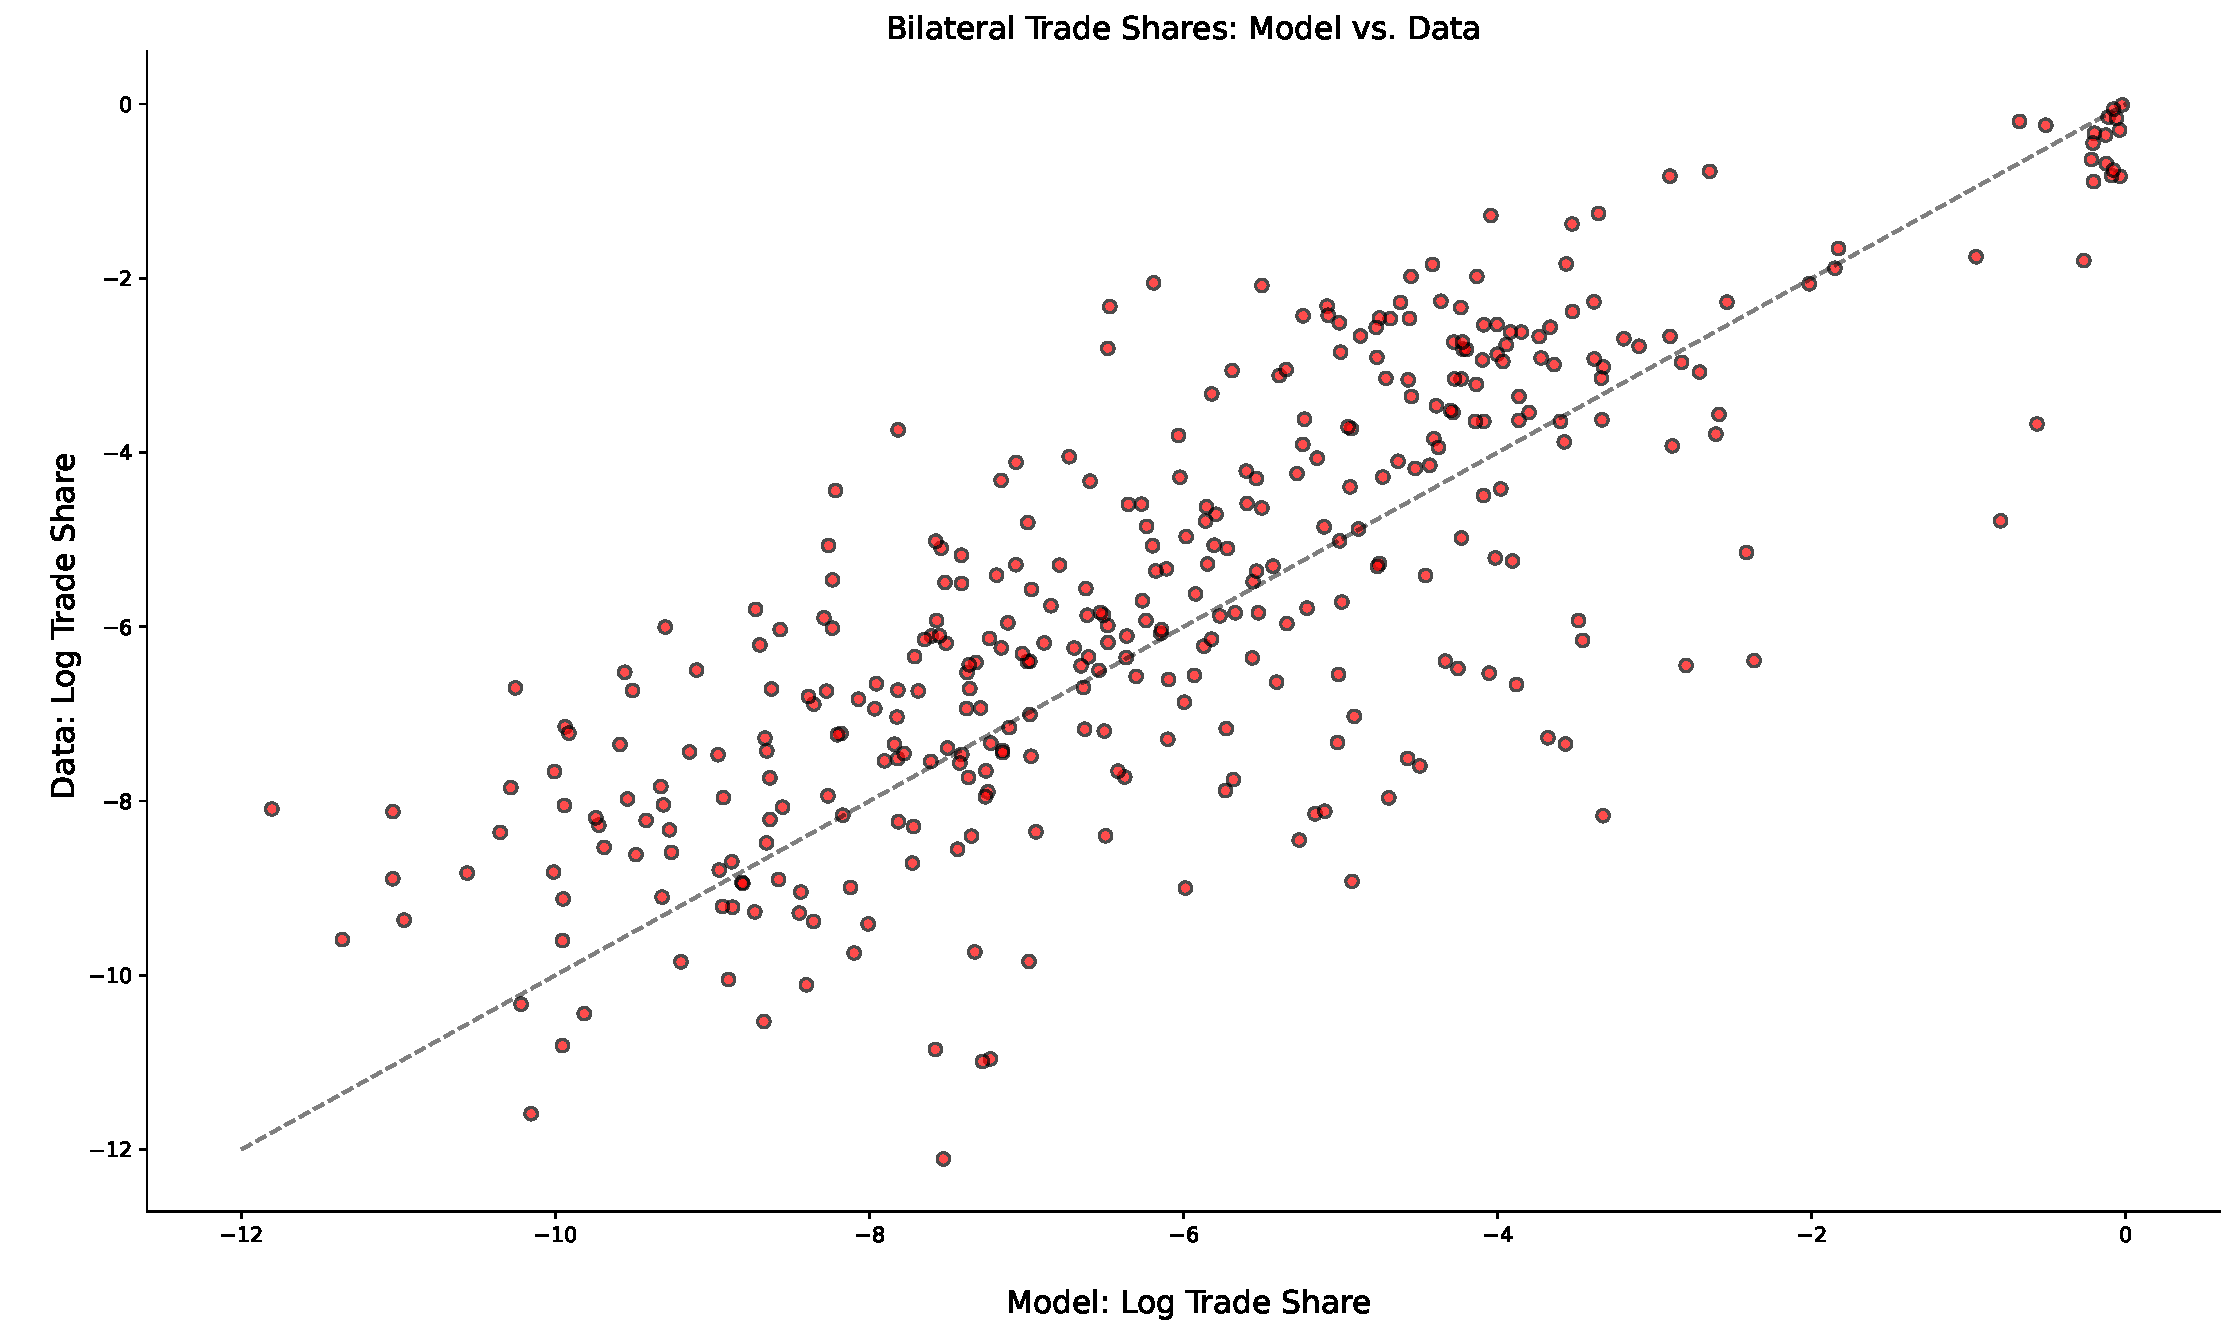
\includegraphics[scale = .5]{./figures/trade-fit.pdf}}
\caption{Bilateral Trade: Model vs. Data}\label{fig:model-fit}
\end{figure}

Table \ref{tb-grav-est} reports another measure of fit and some of the resulting parameter values. The first column is the distance, border, and language moments from the gravity regression run on the data in (\ref{eq:gravity-data}) (and note they exactly correspond with those in the top panel of Table 3 of \citet{eaton2002technology}). The second column reports the moments from the model. Here, they exactly line up and are consistent with the argument in Figure \ref{fig:model-fit}, the fit is good, and the model is replicating geographic patterns of activity seen in the data.

\begin{table}[t]
\small
\begin{center}
\refstepcounter{table}
\setlength {\tabcolsep}{5.5mm}
\renewcommand{\arraystretch}{1.50}\label{tb-grav-est}
\begin{tabular}[t]{l c c c}
\multicolumn{4}{c}{{\normalsize\textbf{Table \ref{tb-grav-est}: Estimation Results}} }
\\\hline \hline
& & \multicolumn{2}{c}{\textbf{HAT-Model}}  \\
\cmidrule(lr){3-4}
Barrier& Moment & Model Fit & Parameter \\
\hline $[0,375)$                &$-3.10 $           & $-3.10 $              & $1.92$           \\
$[375,750)$                     &$-3.67 $           & $-3.67 $              & $2.39$           \\
$[750,1500)$                    &$-4.03 $           & $-4.03 $              & $2.64$           \\
$[1500,3000)$                   &$-4.22 $           & $-4.22 $              & $2.74$           \\
$[3000,6000)$                   &$-6.06 $           & $-6.06 $              & $4.10$           \\
$[6000,\mbox{maximum}]$         &$-6.56 $           & $-6.56 $              & $4.83$           \\
Shared border                   &$\phantom{-}0.30$  & $\phantom{-}0.30$     & $0.92$  \\
Language                        &$\phantom{-}0.51$  & $\phantom{-}0.51$     & $0.85$  \\
EFTA                            &$\phantom{-}0.04$  & $\phantom{-}0.04$     & $0.96$  \\
European Community              &$\phantom{-}0.54$  & $\phantom{-}0.54$     & $0.91$  \\
\hline
\end{tabular}
\\[0.5ex]
\parbox{5.0in}{\footnotesize \textbf{Note:} The first column reports data moments the HAT-model targets. The second reports the model moments. The third column reports the estimated parameter values.}
\end{center}
\end{table}

The final column reports the primitive estimates on the trade cost function. Each value reports the level effect of being in a distance bin or sharing a border, and so on.  So, if two countries are measured to be in the smallest distance bin and share a border, the trade cost between these two countries is $1.92 \times 0.92$ (first row times seventh row). Or, if a country is in the furthest distance bin, its trade cost is 4.83.

Figure \ref{fig:bilateral-elasticities} provides an example of the of trade elasticities that come out of this model. In this figure, I focus on the US and plot each bilateral trade elasticity versus the price a consumer in the US faces when importing a variety from that country. The balls represent the relative size of US imports from that destination. And these elasticities are constructed from the bottom up via the formula in (\ref{eq:trade-elasticity}). The feature that stands out very clearly in Figure \ref{fig:bilateral-elasticities} is that trade elasticities systematically increase with price and decrease with the volume of trade.

\begin{figure}[!t]
\centering{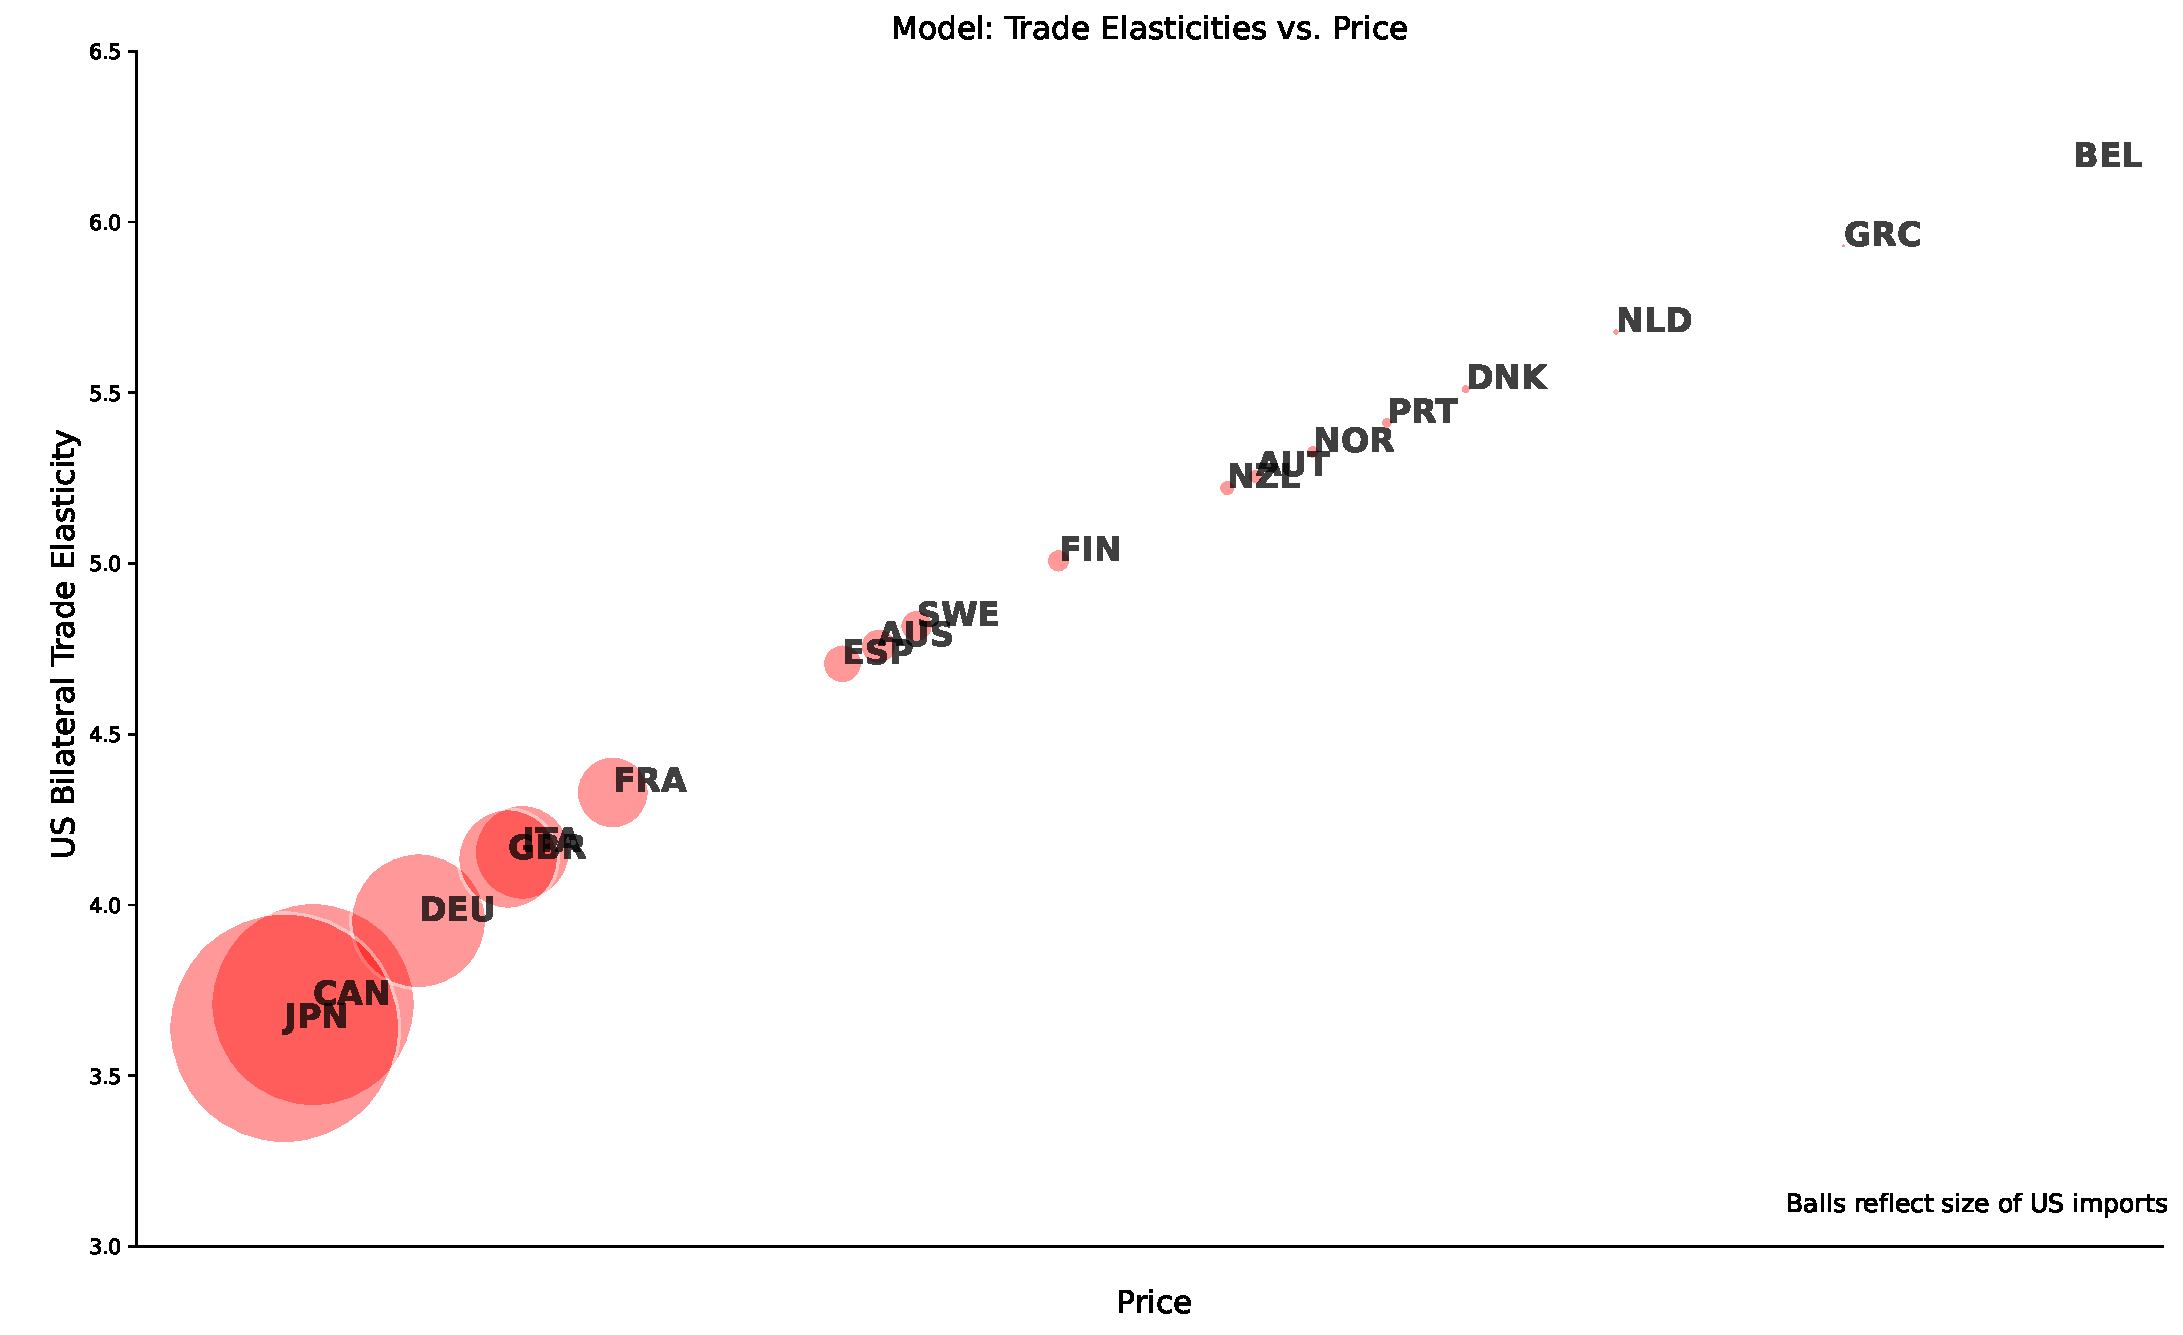
\includegraphics[scale = .5]{./figures/us-elasticity.pdf}}
\caption{Trade Elasticities $-\theta_{us,j}$}\label{fig:bilateral-elasticities}
\end{figure}

At the micro-level, there are two opposing forces giving rise to this aggregate relationship. Per the arguments discussed above around Proposition \ref{prp:GET}, the aggregate bilateral trade elasticity reflects both household-level elasticities $\theta(a,z)$s and a composition effect that works through the expenditure weights $\omega(a,z)$s. Thus, when prices increase as one moves from one source to a less competitive source, there are two competing forces at work: (i) how do micro-level elasticities change, and (ii) how does composition change?

The first force is that as prices increase, \emph{both} rich households' and poor households' elasticities increase. In other words, everyone is more elastic when contemplating a purchase from a more expensive destination. This is a force pushing the model to have elasticities \emph{increase} with price.

The second force | the composition effect| generally works in the opposite direction. As one moves from more cheaper to expensive destinations, less price sensitive households sort into those varieties. Thus, the households purchasing more expensive varieties are the rich, relatively inelastic households. This is a force pushing the model to have elasticities \emph{decrease} with price. \citet{nakamura2010accounting} and \citet*{head2021poor} highlight this composition effect in shaping pass-through.

Which one wins? Figure \ref{fig:bilateral-elasticities} shows that the first force dominates the composition effect. One way to view this result is through the lens of \citeapos{mrazova2017not} language that demand in this model endogenously turns out to be subconvex relative to CES demand, which is equivalent to Marshall's second law of demand. The endogenous part is important as it's not parameterized as in, say, Kimball demand which has become a popular tool to allow for non-constant elasticities. Did the model have to deliver this? Per the arguments above, it's not obvious, as composition effects could have dominated.

There is evidence suggesting that trade elasticities conform to this pattern in my model. Both \citet{novy2013international} and \citet{carrere2020gravity} find that the larger the proxies for the trade elasticities, the less trade there is between two countries. \citet{chen2022gravity} further confirm this idea by finding that trade cost effects are strong for small bilateral relationships and weak or even zero for large trading relationships. Mapping these ideas back into outcomes from my model, a currency union between the US and Canada would likely have a small effect since this is a high volume / low elasticity relationship.

To summarize, the model is replicating geographic patterns of activity seen in the data just as well as a standard constant elasticity trade model. Moreover, households-level heterogeneity in my model leads to an interesting implication that trade elasticities decrease with the volume of trade and this outcome is consistent with some evidence on variable trade elasticities.

\section{The Welfare Gains from Trade}

In this section, I measure the gains from trade and study how they are distributed across households.

\subsection{Measuring Welfare}

In the previous section, I focused on what amount to level changes in utils to understand mechanisms. Here, I define an equivalent variation measure that has more interpretable units, and I use it in the quantitative results.

As a quick refresher, equivalent variation does the following: given that some price change delivers utility level $v'$, equivalent variation asks, ``At the old prices, $p_0$, how much extra income must be provided to be indifferent between $v'$ and $v$?''

To implement this in my model, there are several questions about what the variation should be on, the path, etc. I discuss these questions in the Appendix \ref{apx-sec:measuring-wealfare}. My approach is to look for a constant proportional path of equivalent variation on period wealth (assets and labor income). That is, each period, how much extra wealth should the household be provided to be indifferent at the old prices.

Define the value function of a household at base period prices as
\begin{align}
v_i(a, z ; \ \mathbf{p}),
\end{align}
where the price vector $\mathbf{p}$ includes the price of the different goods, wages, and the interest rate. And the value function for the same states, but at counterfactual prices is
\begin{align}
v'_i(a, z ; \mathbf{p'}), \label{eq:welfare-eqv-cftc}
\end{align}
where I'm evaluating this with the prices prevailing at the new steady state, and hence there are no $t$ subscripts. I focus on steady states, not transition paths. Those may be important, but they add an additional computational challenge, which I've chosen to abstract from for now.

Given these definitions, my equivalent variation measure is a permanent, proportional increase $\tau_{i,a,z}$, at the old prices such that the new level of utility $v'_i$ is achieved:
\begin{align}
v'_i(a,z ; \mathbf{p'}) = v_i(a,z ; \mathbf{p}, \tau_{i, a,z}). \label{eq:welfare-eqv}
\end{align}
This says a household living in country $i$ with states $a,z$ must have its period wealth increased today (and for the infinite future) by the number $\tau_{i,a,z}$. The subscript notation indexes this value by the original type of household I'm looking at, and so there is one number for each type of household with $a,z$ states in country $i$. The $\tau$s that solve (\ref{eq:welfare-eqv}) are my measure of welfare at the household level.

\subsection{Quantitative Results: The Welfare Gains Trade}

This section studies the welfare gains from trade for households in the US under two counterfactual scenarios: (i) a unilateral reduction in trade costs by the US and (ii) a global reduction in trade costs.

The first exercise is a 10 percent reduction in all US import trade costs. That is, $d_{us,j}$ is shifted down for all $j$ sources by 10 percent. Figure \ref{fig:welfare-households} reports the welfare gains across households. Households are binned by quantiles of the initial distribution of consumption expenditure, and the y-axis reports the average gains within each bin. The red bars report the baseline model, and the blue bars report the $\log$ preference case when, per Corollary \ref{prp:seperation}, heterogeneous price sensitivity does not operate.

\begin{figure}[!t]
\centering{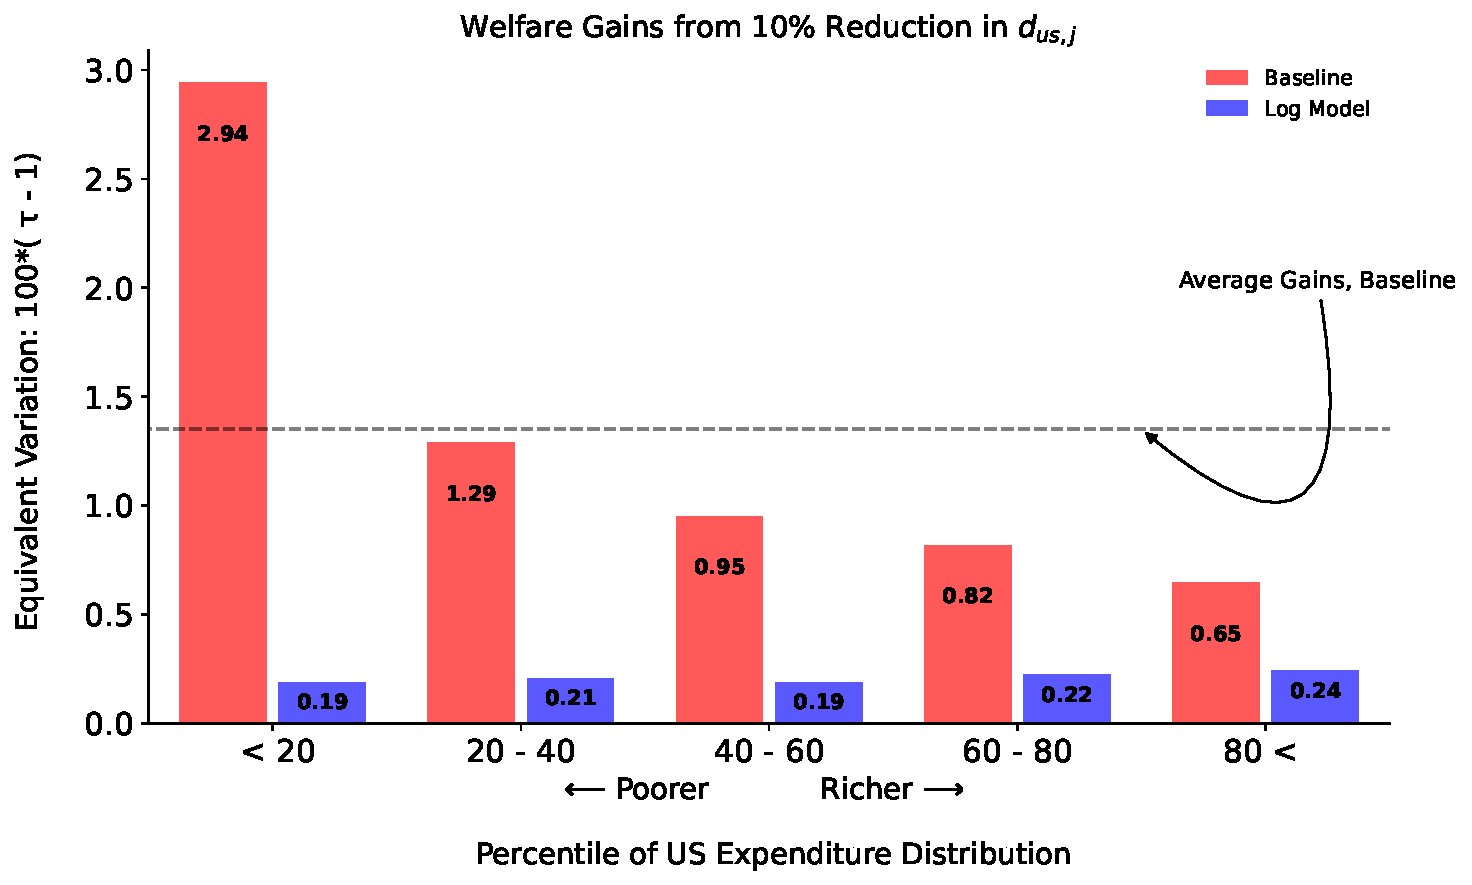
\includegraphics[scale = 0.65]{./figures/ge-welfare-household-vs-log.pdf}}
\caption{US Welfare Gains from a 10\% Reduction in $d_{us,j}$ }\label{fig:welfare-households}
\end{figure}

Figure \ref{fig:welfare-households} shows that gains from trade are strongly pro-poor. Across income brackets, the poorest households gain four and a half times more from trade than the richest households (2.93 percent vs. 0.65 percent).

The blue bars in Figure \ref{fig:welfare-households} help answer why the gains are pro-poor. These bars are the gains in the $\log$ preference model. Recalling Corollary \ref{prp:seperation}, the gains from substitution in the $\log$ preference model are the same across households. Thus, any heterogeneous gains arise from changes in factor prices and potential effects from borrowing constraints. The blue bars in Figure \ref{fig:welfare-households} illustrate that the gains from trade in the $\log$ preference model are nearly uniform across the distribution.\footnote{The level of gains is lower as well, but this is because trade increases by less in the log model. Adjusting the change in the $d_{us,j}$ to generate an equivalent increase in trade in the $\log$ model leads to the same conclusion: the gains from trade are virtually the same across rich and poor households.}

Behind the heterogeneity in the gains from substitution, the key issue is heterogeneous price elasticities. As discussed around equation (\ref{eq:gains-substitution}) there are essentially two issues are at play determining how this aspect of the model leads to heterogeneous gains across households: (i) how exposed a household is to trade and (ii) how households value a price reduction. The model was calibrated so that exposure was equal across the income distribution, and thus (i) is not leading to heterogeneous gains from trade.  In contrast, the model was designed and calibrated to match the fact that poor households are very elastic with respect to price, and thus they strongly value a price reduction. So the second force is the key component driving the pro-poor aspect of these gains from trade.\footnote{For example, I calibrated the model without quality shifters delivering a pattern of micro-level expenditure shares with the poor unexposed to trade that is similar to Figure \ref{fig:micro-trade}. In this case, the gains are flat across the income distribution (except for the very poorest) because the pro-poor nature of the elasticity effects are off-set by exposure.}

A secondary implication of Figure \ref{fig:welfare-households} is that the average gains from trade are much larger than representative agent benchmarks. The dashed line in Figure \ref{fig:welfare-households} shows that the average gain is 1.35 percent. In contrast, a calculation of \citet{arkolakis2012new} off of the change in the US import share and an elasticity equal to the average trade-weighted elasticity in the baseline model (see Figure \ref{fig:bilateral-elasticities}) yields a gain of only 0.45 percent. This is a third of the size (1.35 vs. 0.45) of the average gains in my model.

My model delivers larger average gains is mainly because of the gains in the bottom part of the income distribution. Looking at Figure \ref{fig:welfare-households}, I note that the gains from trade for the rich households are quantitatively similar to those that would come out of my \citet{arkolakis2012new}-style calculation. However, for poor households, the gains are really big. Then, when averaging over modest gains for rich households and large gains for poor households, the average gains in my model are three times larger.

Per the results in Proposition \ref{prp:gains-trade}, what is the role of factor prices? It seems small, but I'll admit that it is hard to qualitatively separate out in a clean way. In the counterfactual, the ratio of $R/w$ increases by about 4.6 percent, and this effect in the $\log$ model is quantitatively similar as well. The reason for the decline is that demand for US goods (and hence labor) falls as households substitute into foreign goods, and so US wages fall. The interest rate is essentially globally determined and increases only slightly. The implication is that there is a counteracting pro-rich force behind Figure \ref{fig:welfare-households}. That is, for those holding positive assets, these moves in factor prices are beneficial and for debtors these moves hurt. And this is why I suspect the gains are slightly pro-rich in the $\log$ model. But they are very slightly so, and hence, this is my argument that moves in factor prices are not strongly determining if the gains are pro-rich or -poor.

The next exercise is a global reduction in trade costs by 10 percent. One virtue of this exercise connects with the previous paragraph. Global trade cost reductions mute changes in factor prices since demand rises for all products, and so wages and interest rates don't adjust much. In addition to illustrating the gains from globalization, it also helps isolate the role that factor prices play.

\begin{figure}[!t]
\centering{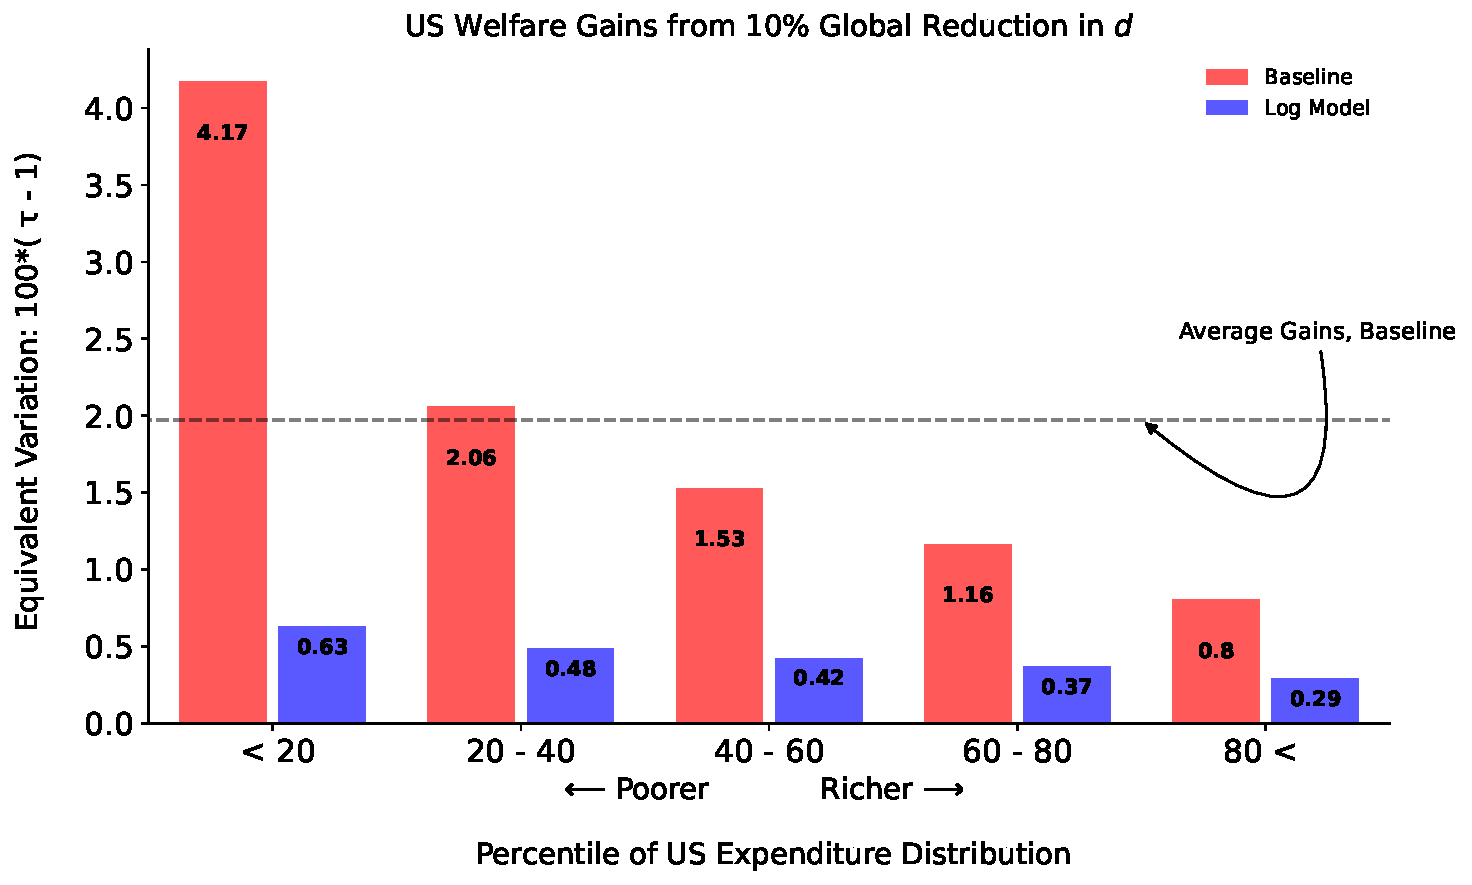
\includegraphics[scale = 0.65]{./figures/global-welfare-household-vs-log.pdf}}
\caption{US Welfare Gains from a 10\% Reduction in $d$ }\label{fig:welfare-households-global}
\end{figure}

Figure \ref{fig:welfare-households-global} reports the gains from trade. The gains are slightly more pro-poor than those of the previous results, with the poorest households gaining a bit more than five times more than the richest households (4.17 percent vs. 0.8 percent). In this sense, globalization is an even stronger force for the poor than the unilateral trade-liberalization that the previous exercise mimics. Because the gains behind globalization are pro-poor, but the gains for the rich are \citet{arkolakis2012new}-like, the average gains across are much larger than representative agent benchmarks. This can be seen with the average gain being about 2 percent for a global reduction in trade costs. The \citet{arkolakis2012new} benchmark is 0.73 percent which is quantitatively similar to the gains for the richest households in the economy of 0.80 percent.\footnote{The global reduction also provides a point of comparison to the quantitative results of \citet{auer2022unequal}. For a 10 percent increase in prices, they find that the difference in the gains between the rich and poor is 0.8 percentage points (their Table 8). Here things are substantially larger; there is a 3 percentage point difference between the rich and poor.}


The blue bars in Figure \ref{fig:welfare-households-global} illustrate the gains in the $\log$ preference model. As with the unilateral reduction, the gains are uniformly smaller. In contrast to the unilateral reduction, there is now a pro-poor angle to the gains from trade. This is not about heterogeneous gains from substitution, but must be working through changes in factor prices and the role of the borrowing constraint. As discussed above, because factor prices are not changing that much (less than one percent in both the baseline and $\log$ model), this suggests that the relaxation of the borrowing constraint is a very modest force driving pro-poor gains, even in the absence of heterogeneous price elasticities.

\section{Conclusion}

This paper developed a model focused on the idea of heterogeneous price elasticities. From my perspective, a lot of stuff came out of this exercise, such as how heterogeneous elasticities connect with consumption inequality and in turn shape the gains from trade, and how preferences and market incompleteness shape these outcomes. This framework also became a laboratory to illustrate how a multi-country heterogenous agent trade model could be computed and calibrated to match the bilateral pattern of trade.

Perhaps most surprising is how potent heterogeneous price elasticities are quantitatively, with my finding of large pro-poor gains from trade. And the core idea is not that prices decline more for poor households vs. rich households. It's that, in layman's terms, a dollar price reduction is of higher value to the poor than the rich.

This paper does open up many more questions. One question that I pursue in \citet{waughoptimal} is the optimal pattern of trade and what it looks like relative to the pattern of trade we observe. A related question is if and how can trade policy improve outcomes. The third question is about the interaction between trade in goods and trade in assets.  Admittedly, I under-explore this point in this paper. But piecing together the trade side and finance side of international economics is an area ripe for future research.


\appendix

\clearpage
\newpage

\begin{center}
\textbf{\Large Appendix} \\
\textbf{For Online Publication}
\end{center}

\addcontentsline{toc}{section}{Appendices}

\section{The HA Trade Elasticity}

My definition of the trade elasticity is the partial equilibrium response of imports from $j$ relative to domestic consumption due to a permanent change in trade costs. By partial equilibrium, I mean that wages, interest rates, and the distribution of agents are fixed at their initial equilibrium values. This is consistent with the definition of the trade elasticity in, say, \citet{arkolakis2012new} and \citet{simonovska2014elasticity}. By permanent, I mean that the change in trade costs is for the indefinite future and that households correctly understand this. Consistent with this discussion and the notation below, I compute the partial derivatives (not total) of objects with respect to trade costs.

Mathematically, the trade elasticity equals the difference between the elasticities for how trade between $i$ and $j$ change minus how home trade changes
\begin{align}
\frac{\partial ( M_{ij} / M_{ii} )}{\partial d_{ij}} \times \frac{d_{ij}}{( M_{ij} / M_{ii} )} =& \frac{\partial M_{ij} / M_{ij}}{\partial d_{ij} / d_{ij}}  - \frac{\partial M_{ii} / M_{ii}}{\partial d_{ij} / d_{ij}}.
\label{apx-eq:def_trade_elasticity}
\end{align}
The change in imports between $i$ and $j$ with respect to a change in trade costs is
\begin{align}
\frac{\partial  M_{ij}}{\partial d_{ij}} = \int_{a,z} \bigg \{\frac{\partial p_{ij}}{\partial d_{ij}} c_{i}(a,z,j) \pi_{ij}(a,z) +  \frac{\partial c_{i}(a,z,j)}{\partial d_{ij}} p_{ij} \pi_{ij}(a,z) +
 \frac{\partial \pi_{ij}(a,z)}{\partial d_{ij}} p_{ij}c_{i}(a,z,j) \bigg \} L_i \lambda_{i}(a,z) da \ dz.
\end{align}
Divide the stuff inside the brackets by household-level imports, $p_{ij}c_{i}(a,z,j)\pi_{ij}(a,z)$, and multiply on the outside, giving
\begin{align}
\frac{\partial  M_{ij}}{\partial d_{ij}} = \int_{a,z}  \bigg \{ \frac{\partial p_{ij}/p_{ij}}{\partial d_{ij}}  + \frac{\partial c_{i}(a,z,j)/ c_{i}(a,z,j)}{\partial d_{ij}} +
 \frac{\partial \pi_{ij}(a,z) / \pi_{ij}(a,z)}{\partial d_{ij}}  \bigg \} p_{ij}c_{i}(a,z,j)\pi_{ij}(a,z) L_i \lambda_{i}(a,z)da \ dz.
\end{align}
Define the following ``weight,'' which is the share of goods that households with states $a,z$ account for in total expenditures from $j$ as
\begin{align}
\omega_{ij}(a,z) = \frac{p_{ij}c_{i}(a,z,j)\pi_{ij}(a,z) L_i \lambda_{i}(a,z)}{M_{ij}},
\end{align}
where the sum of $\omega_{ij}(a,z)$ over states $a,z$ equals one. This gives a nice expression for the import elasticity:
\begin{align}
\frac{\partial  M_{ij} / M_{ij}}{\partial d_{ij} / d_{ij}} = 1 + \int_{a,z} \bigg \{ \underbrace{ \frac{\partial c_{i}(a,z,j)/ c_{i}(a,z,j)}{\partial d_{ij} / d_{ij}} }_{\theta_{ij}(a,z)^{I}}+
\underbrace{\frac{\partial \pi_{ij}(a,z) / \pi_{ij}(a,z)}{\partial d_{ij} / d_{ij}} }_{\theta_{ij}(a,z)^{E}} \bigg \} \omega_{ij}(a,z)da \ dz,
\end{align}
or more succinctly,
\begin{align}
\frac{\partial  M_{ij} / M_{ij}}{\partial d_{ij} / d_{ij}} = 1 + \int_{a,z} \bigg \{ \theta_{ij}(a,z)^{I} + \theta_{ij}(a,z)^{E} \bigg \}\omega_{ij}(a,z)da \ dz
\end{align}
where the elasticity of aggregate imports into $i$ from $j$ is a weighted average of several effects. The value of one out in front arises from the complete pass-through of changes in trade costs to changes in prices. Then, the first term within the brackets is the intensive margin $\theta_{ij}(a,z)^{I}$ | that is how much quantities change conditional on choosing to consume variety $j$. The next term $\theta_{ij}(a,z)^{E}$ represents the extensive margin | that is how the choice probabilities change.

To complete the derivation, I derive the own-imports term, which is similar, with
\begin{align}
\frac{\partial  M_{ii}}{\partial d_{ij}} = \int_{a,z} \bigg \{ \underbrace{\frac{\partial p_{ii}}{\partial d_{ij}} c_{i}(a,z,i) \pi_{ii}(a,z)}_{ \ = \ 0} +  \frac{\partial c_{i}(a,z,i)}{\partial d_{ij}} p_{ii} \pi_{ii}(a,z) + \frac{\partial \pi_{ii}(a,z)}{\partial d_{ij}} p_{ii}c_{i}(a,z,i) \bigg \} L_i \lambda_{i}(a,z)da \ dz,
\end{align}
where the first term is zero because this is a partial equilibrium elasticity and hence $p_{ii}$ is not changing with $d_{ij}$. After constructing the proper weights and converting everything to elasticity form, I have
\begin{align}
\frac{\partial  M_{ii} / M_{ii}}{\partial d_{ij} / d_{ij}} = \int_{a,z} \bigg \{ \theta_{ii,j}(a,z)^{I} + \theta_{ii,j}(a,z)^{E} \bigg \}\omega_{ii}(a,z)da \ dz,
\end{align}
where the $ii, j$ notation means that $\theta_{ii,j}(a,z)^{I}$ reflects how the intensive margin adjusts, conditional on a $ii$ choice, given a change in $ij$ price. Similarly, $\theta_{ii,j}(a,z)^{E}$ represents how the $ii$ choice probability changes given the $ij$ change in price.

Proposition \ref{prp:GET} then follows.

\subsection{Connecting Elasticities with Household Behavior}

To derive the \textbf{intensive margin elasticity}, start from the households' budget constraint and differentiate consumption of variety $j$ with respect to price $p_{ij}$
\begin{align}
\underbrace{\frac{\partial c_{i}(a,z,j)/ c_{i}(a,z,j)}{\partial d_{ij} / d_{ij}}}_{\theta_{ij}(a,z)^{I}} &= \bigg [-\frac{\partial g_{i}(a,z,j)/ p_{ij}c_{i}(a,z,j)}{\partial p_{ij}/ p_{ij}} - 1 \bigg ]\frac{\partial p_{ij}/p_{ij}}{\partial d_{ij}/ d_{ij}},
\label{eq:apx-intensive-margin}
\end{align}
where recall that $g_{i}(a,z,j)$ is the policy function mapping states into asset holdings next period $a'$.

To derive the \textbf{extensive margin elasticity}, start from the definition of the choice probability and
\begin{align}
\underbrace{ \frac{\partial \pi_{ij}(a,z) / \pi_{ij}(a,z)}{\partial d_{ij} / d_{ij}} }_{\theta_{ij}(a,z)^{E}} &= \frac{1}{\sigma_{\epsilon}}\frac{\partial v_{i}(a, z, j)}{\partial d_{ij}/d_{ij}} -  \frac{\partial \Phi_{i}(a,z) / \Phi_{i}(a,z)}{\partial d_{ij}/d_{ij}}.
\label{eq:apx-extensive-margin}
\end{align}
I then use the following arguments to unpack how the value function $v_{i}(a, z, j)$ changes:
{\small
\begin{align}
\frac{\partial v_{i}(a,z,j)}{\partial d_{ij}/d_{ij}}  =& -u'(c_{i}(a,z,j))c_{i}(a,z,j) + \bigg [ -\frac{u'(c_{i}(a,z,j))}{p_{ij}}\frac{\partial g_{i}(a,z,j)}{\partial p_{ij}/ p_{ij}} \bigg ]\frac{\partial p_{ij}/p_{ij}}{\partial d_{ij}/ d_{ij}}  \\
\nonumber \\
&+ \beta \mathrm{E} \bigg \{\frac{\partial v}{\partial a'}\frac{\partial g_{i}(a,z,j)}{\partial p_{ij}/ p_{ij}}\frac{ \partial p_{ij}/ p_{ij}}{\partial d_{ij}/ d_{ij}} +  \frac{\partial v(g_{i}(a,z,j),z')}{\partial p_{ij}/ p_{ij}}\frac{ \partial p_{ij}/ p_{ij}}{\partial d_{ij}/ d_{ij}} \bigg \},
\end{align}}
which can then be further expressed in terms of the Euler equation (which I derive below in equation (\ref{eq:apx-euler-equation})):
{\small
\begin{align}
\frac{\partial v_{i}(a,z,j)}{\partial d_{ij}/d_{ij}}  =& -u'(c_{i}(a,z,j))c_{i}(a,z,j) \label{eq:apx-first-term}\\
\nonumber \\
&+ \underbrace{\bigg \{ -\frac{u'(c_{i}(a,z,j))}{p_{ij}} + \beta \mathbb{E} \bigg [ -\sigma_{\epsilon} \frac{\partial \pi_{ii}(a',z') / \pi_{ii}(a',z')}{\partial a'} + u'(c_{i}(a',z',i))R_{i} \bigg ] \bigg \} }_{\mbox{Euler equation in (\ref{eq:apx-euler-equation})}} \frac{\partial g_{i}(a,z,j)}{\partial d_{ij}/ d_{ij}}\\
\nonumber \\
&+  \beta \mathbb{E}\frac{\partial v_{i}(a',z')}{\partial d_{ij}/ d_{ij}}.
\end{align}}
The term in the second line is the Euler equation multiplied by how assets change. This term should be zero for small changes. The basic argument is that either the Euler equation holds and thus this term is zero, or it does not hold, but then households can't adjust asset holdings and then the outside part is zero. And for small changes households on the margin of a binding constraint or not are on the margin and don't matter. I discuss this more in depth below, in the section dealing with the welfare gains calculation.

To add some clarity to this expression, assume the number of countries is large. This assumption implies that the $\partial \Phi$ term in (\ref{eq:apx-extensive-margin}) is zero or approximately so. Next, because the ex-ante value function next period $v_{i}(a',z')$ is just a function of $\Phi$ (see its definition in (\ref{eq:big-phi})),  hence, the large number of countries implies future effects don't matter or approximately so. Altogether, these observations give
\begin{align}
\theta_{ij}(a,z)^{E} \approx -\frac{1}{\sigma_{\epsilon}}\bigg[u'(c_{i}(a,z,j))c_{i}(a,z,j)\bigg]. \label{apx-eq:extensive-margin-large}
\end{align}
From here, I can connect (\ref{apx-eq:extensive-margin-large}) with things like relative risk aversion and the marginal propensity to consume. The thought experiment here is see how (\ref{apx-eq:extensive-margin-large}) changes with wealth:
\begin{align}
\frac{\partial (u'(c_{i}(a,z,j))c_{i}(a,z,j))}{\partial a} =& u''(c_{i}(a,z,j))\frac{\partial c_{ij}}{\partial a}c_{i}(a,z,j) + u'(c_{i}(a,z,j))\frac{\partial c_{ij}}{\partial a} \\
\nonumber \\
&= \frac{\partial c_{ij}}{\partial a}\bigg[u''(c_{i}(a,z,j))c_{i}(a,z,j) + u'(c_{i}(a,z,j)) \bigg] \\
\nonumber\\
&= u'(c_{i}(a,z,j))\times \mathbf{MPC}_{ij}(a,z,j) \times \bigg[-\gamma_{i}(a,z,j) + 1\bigg]. \label{eq:apx-elasticity-mpc}
\end{align}
And just to emphasize how this works, it's a derivative of $u'(c_{i}(a,z,j))c_{i}(a,z,j)$. So as assets go up, with $\gamma > 1$ this implies that $u'(c_{i}(a,z,j))c_{i}(a,z,j)$ goes down. And this is a force for things to be less elastic for rich guys. As assets go down, this implies that $u'(c_{i}(a,z,j))c_{i}(a,z,j)$ goes up, and this is a force for poor guys to be more elastic.

To complete everything, I derive how the home intensive margin changes and how the home choice probability changes. This last calculation is also important in the sense that it shows up in the welfare expressions. The home intensive margin is
\begin{align}
\underbrace{\frac{\partial c_{i}(a,z,i)/ c_{i}(a,z,j)}{\partial d_{ij} / d_{ij}}}_{\theta_{ii,j}(a,z)^{I}} &= -\frac{\partial g_{i}(a,z,i)/ p_{ii}c_{i}(a,z,i)}{\partial d_{ij}/ d_{ij}},
\end{align}
which makes an interesting point that even the home intensive margin responds because asset holdings will adjust to the change in price $p_{ij}$. The next step is how the home choice probability respond to changes in trade frictions.
\begin{align}
\underbrace{\frac{\partial \pi_{ii}(a,z) / \pi_{ii}(a,z) }{\partial d_{ij} / d_{ij}}}_{\theta_{ii,j}(a,z)^{E}} = \frac{1}{\sigma_{\epsilon}}\frac{\partial v_{i}(a,z,i)}{\partial d_{ij}/d_{ij}} - \frac{\partial \Phi_{i}(a,z) / \Phi_{i}(a,z)}{\partial d_{ij}/d_{ij}}.
\end{align}
Then, the derivative $\Phi_{i}$ term takes on a unique property where
\begin{align}
\frac{\partial \Phi_{i}(a,z) / \Phi_{i}(a,z)}{\partial d_{ij}/d_{ij}} = \sum_{j} \pi_{ij}(a,z) \frac{1}{\sigma_{\epsilon}}\frac{\partial v_{i}(a,z,j)}{\partial d_{ij}/d_{ij}},
\end{align}
which takes on this flavor of exposure (which are the choice probabilities) times how the household's valuations across the goods change (as represented by the value functions). Then, expressing things all relative to how the home valuation changes I have
\begin{align}
\frac{\partial \pi_{ii}(a,z) / \pi_{ii}(a,z) }{\partial d_{ij} / d_{ij}} = \frac{1}{\sigma_{\epsilon}} \sum_{j} \pi_{ij}(a,z) \bigg[ \frac{\partial v_{i}(a,z,i)}{\partial d_{ij}/d_{ij}} - \frac{\partial v_{i}(a,z,j)}{\partial d_{ij}/d_{ij}} \bigg].
\label{eq:apx-change-home-choice}
\end{align}

\section{HA Gains from Trade}\label{apx-sec:gains-trade}


This section derives the gains from a permanent change in trade costs, across steady states. As discussed in the main body of the text, I derive these gains across steady states where I'm thinking a situation where the change is small and there is an immediate jump to the new steady state.  Unlike the trade elasticity, I take total derivatives that encompass general equilibrium changes in wages and interest rates.

The analysis focuses on how household-level welfare changes. To characterize this, I make the use of the observation in equation (\ref{eq:log_sum-home}) that I can express the ex-ante value function in only in terms of home choice $ii$ values and then recursively push forward. In other words, I can compute the change in the ex-ante value function \emph{as if} the household consumed only the home good for the infinite future.

How does household-level welfare change? Recall that the value function (with the expectation taken over the different preference shocks) is
\begin{align}
v_i(a, z) =  \sigma_{\epsilon} \log \left\{ \sum_{j'} \exp \left( \frac{  v_{i}(a, z, j')}{\sigma_{\epsilon}} \right) \right\}.
\label{eq:apx-epsilon-vfun}
\end{align}
Notice that I can substitute out the sum part (\ref{eq:apx-epsilon-vfun}) with the home value function relative to the micro-level ``home choice'' so that
\begin{align}
\pi_{ii}(a, z) = \exp \left( \frac{ v_{i}(a, z, i) }{\sigma_{\epsilon}} \right) \Bigg / \sum_{j'} \exp \left( \frac{ v_{i}(a, z, j') }{\sigma_{\epsilon}} \right), \\
\nonumber \\
\pi_{ii}(a, z) \times \sum_{j'} \exp \left( \frac{ v_{i}(a, z, j') }{\sigma_{\epsilon}} \right) = \exp \left( \frac{ v_{i}(a, z, i) }{\sigma_{\epsilon}} \right), \\
\nonumber \\
\sum_{j'} \exp \left( \frac{ v_{i}(a, z, j') }{\sigma_{\epsilon}} \right) = \exp \left( \frac{ v_{i}(a, z, i) }{\sigma_{\epsilon}} \right) \Bigg / \pi_{ii}(a, z).
\label{eq:apx-homeshare-vfun}
\end{align}
Then, substituting (\ref{eq:apx-homeshare-vfun}) into the value function in (\ref{eq:apx-epsilon-vfun}) gives
\begin{align}
v_i(a, z) =  \sigma_{\epsilon} \log \left\{ \frac{ \exp \left( \frac{  v_{i}(a, z, i)}{\sigma_{\epsilon}}\right )}{\pi_{ii}(a,z)}  \right\},
\label{eq:apx-homeshare-vfun2}
\end{align}
and recall that the home choice value function that enters into (\ref{eq:apx-homeshare-vfun2}) is
\begin{align}
v_{i}(a, z, i) = u(c_{i}(a,z,i)) + \beta \mathbb{E} v_{i}(g_{i}(a,z,i),z),
\end{align}
where the expectation operator is over the $z$s and the $v_{i}$ is the same value function as in (\ref{eq:apx-epsilon-vfun}) so the taste shocks are integrated out. Expanding out (\ref{eq:apx-homeshare-vfun2}) allows for the $v_i$ value function to be represented as
\begin{align}
v_i(a, z) = -\sigma_{\epsilon} \log \pi_{ii}(a,z) + u(c_{i}(a,z,i)) + \beta \mathbb{E} v_{i}(g_{i}(a,z,i),z).
\label{eq:apx-home-valuefun}
\end{align}
Now, everything is written with respect to the home choice. What is going on is that the home choice $\pi_{ii}$ summarizes the expected value of those shocks and their benefits. There is no need to explicitly carry around the $v_{ij}$s. This is essentially the dynamic analog to Equation (15), Footnote 42 of \citet{eaton2002technology} and \citet{arkolakis2012new}.

Lastly, to facilitate interpretation, compute the Euler equation associated with asset holdings when the borrowing constraint does not bind. This Euler equation is
\begin{align}
\frac{u'(c_{i}(a, z, i))}{p_{ii}} = \beta \mathrm{E}_{z'} \left[ -\sigma_{\epsilon} \frac{\partial \pi_{ii}(a',z') / \pi_{ii}(a',z')}{\partial a'} + \frac{u'(c_{i}(a', z', i))R_i}{p_{ii}} \right]. \nonumber
\end{align}
This equation is derived below in (\ref{apx-eq:homechoice-euler}).

Now, the strategy is to totally differentiate (\ref{eq:apx-home-valuefun}) with respect to trade costs and use the recursive structure to iterate forward and construct the change across time. Totally differentiating the value function gives
{\small
\begin{align}
\frac{\mathrm{d} v_i(a, z)}{\mathrm{d} d_{ij} / d_{ij}} =& \nonumber  \\
\nonumber \\
-\sigma_{\epsilon} & \frac{\mathrm{d} \pi_{ii}(a,z) / \pi_{ii}(a,z)}{\mathrm{d}d_{ij} / d_{ij}}  + u'(c_{i}(a,z,i)) \bigg[ \frac{\mathrm{d} w_{i} / p_{ii}}{\mathrm{d} d_{ij} / d_{ij}}z  +  \frac{\mathrm{d} R_{i} / p_{ii}}{\mathrm{d} d_{ij} / d_{ij}} a  \bigg] \\
\nonumber  \\
& - \frac{u'(c_{i}(a,z,i))}{p_{ii}}\frac{\mathrm{d} g_{i}(a,z,i)}{\mathrm{d} d_{ij} / d_{ij}} + \beta \mathbb{E}_{z'} \frac{\mathrm{d} v_i(g_{i}(a,z,i), z')}{\mathrm{d} d_{ij} / d_{ij}}.
\end{align}
}
Then the derivative of the continuation value function is
{\small
\begin{align}
\frac{\mathrm{d} v_i(g(a,z,i), z')}{\mathrm{d} d_{ij} / d_{ij}} = &  \underbrace{\bigg [-\sigma_{\epsilon} \frac{\partial \pi_{ii}(a',z') / \pi_{ii}(a',z')}{\partial a'} + \frac{u'(c_{i}(a',z',i))R_{i}}{p_{ii}} \bigg ]}_{\frac{\partial v_i(g_{i}(a,z,i), z')}{\partial a}}\frac{\mathrm{d} g_{i}(a,z,i)}{\mathrm{d} d_{ij} / d_{ij}} \ \ + \\
\nonumber \\
-\sigma_{\epsilon} & \frac{\mathrm{d} \pi_{ii}(a',z') / \pi_{ii}(a',z')}{\mathrm{d}d_{ij} / d_{ij}}  + u'(c_{i}(a',z',i)) \bigg[ \frac{\mathrm{d} w_{i} / p_{ii}}{\mathrm{d} d_{ij} / d_{ij}}z'  +  \frac{\mathrm{d} R_{i} / p_{ii}}{\mathrm{d} d_{ij} / d_{ij}} a'  \bigg] + \\
\nonumber \\
& - \frac{u'(c_{i}(a',z',i))}{p_{ii}}\frac{\mathrm{d} g_{i}(a',z',i)}{\mathrm{d} d_{ij} / d_{ij}}
+ \beta \mathbb{E}_{z'} \frac{\mathrm{d} v_i(g_{i}(a',z',i), z'')}{\mathrm{d} d_{ij} / d_{ij}}.
\end{align}
}
And collect terms so
{\small
\begin{align}
\frac{\mathrm{d} v_i(a, z)}{\mathrm{d} d_{ij} / d_{ij}} =& \underbrace{-\sigma_{\epsilon} \frac{\mathrm{d} \pi_{ii}(a,z) / \pi_{ii}(a,z)}{\mathrm{d}d_{ij} / d_{ij}}}_{\mathbf{A(a,z)}} \\
\nonumber \\
& + \underbrace{u'(c_{i}(a,z,i)) \bigg[ \frac{\mathrm{d} w_{i} / p_{ii}}{\mathrm{d} d_{ij} / d_{ij}}z  +  \frac{\mathrm{d} R_{i} / p_{ii}}{\mathrm{d} d_{ij} / d_{ij}} a  \bigg]}_{\mathbf{B(a,z)}}  \\
\nonumber \\
& + \underbrace{\bigg \{- \frac{u'(c_{i}(a,z,i))}{p_{ii}} + \beta \mathbb{E}_{z'} \bigg [-\sigma_{\epsilon} \frac{\partial \pi_{ii}(a',z') / \pi_{ii}(a',z')}{\partial a'} + \frac{u'(c_{i}(a',z',i))R_{i}}{p_{ii}} \bigg ] \bigg \}\frac{\mathrm{d} g_{i}(a,z,i)}{\mathrm{d} d_{ij} / d_{ij}}}_{\textbf{C(a,z)}} \\
\nonumber \\
& + \beta \mathbb{E}_{z'} \bigg \{ -\sigma_{\epsilon} \frac{\mathrm{d} \pi_{ii}(a',z') / \pi_{ii}(a',z')}{\mathrm{d}d_{ij} / d_{ij}} +  u'(c_{i}(a',z',i)) \bigg[ \frac{\mathrm{d} w_{i} / p_{ii}}{\mathrm{d} d_{ij} / d_{ij}}z'  +  \frac{\mathrm{d} R_{i} / p_{ii}}{\mathrm{d} d_{ij} / d_{ij}} a' \bigg] \ \  \ldots
\label{eq:apx-welfare-vterms}
\end{align}
}
Let me walk through the interpretation of each term.
\begin{itemize}
\item[\textbf{A(a,z) -}] The term here $-\sigma_{\epsilon} \frac{\mathrm{d} \pi_{ii}(a,z) / \pi_{ii}(a,z)}{\mathrm{d}d_{ij} / d_{ij}}$ is a gains from substitution term. I discuss this further below, but it summarizes two effects: (i) how exposed the household is to market $j$, and an effect from a elasticity term.

\item[\textbf{B(a,z) -}] The second term $\bigg[ \frac{\mathrm{d} w_{i} / p_{ii}}{\mathrm{d} d_{ij} / d_{ij}}z  +  \frac{\mathrm{d} R_{i} / p_{ii}}{\mathrm{d} d_{ij} / d_{ij}} a  \bigg]$ is how a reduction in trade costs affects factor prices | the wage relative to the price of the home good and the interest rate relative to the price of the home good. And these effects are all valued at that household's marginal utility of consumption.

    Two more observations: first, with perfect competition $\frac{w_i}{p_{ii}} = A_{i}$ from (\ref{eq:marginal-product}). And thus, $\frac{\mathrm{d} w_{i} / p_{ii}}{\mathrm{d} d_{ij} / d_{ij}} = 0$, so households are perfectly ``hedged'' from any effect on labor earnings. Second, there is an effect from how the ``real'' interest rate changes. Here real is in quotes because this is real in units of the home good (and per the observation above, this boils down to the change in the interest rate relative to the wage rate). And because the $a$ can take on positive or negative values, this is a force that could in principle lead to losers from trade.

\item[\textbf{C(a,z) -}]  The third term is about changes in asset holdings. For the small / local changes that I'm considering, it should zero out. But for larger changes this term could be relevant. Let me expand upon this.

    First, notice that the inside-the-bracket term is the Euler equation from (\ref{apx-eq:homechoice-euler}) and it's multiplied by the change in policy function. The idea is that if the household is unconstrained, then the inside-the-bracket term is zero as there is no gain through changes in asset behavior. Asset holdings are already chosen optimally so that margins are equated; thus, on the margin, any benefit of lower trade costs on changes in asset behavior is zero.

    Now in this economy, this term may not be zero because of borrowing-constrained households; thus, the inside-the-bracket term is positive. However, notice how the outside brackets are multiplied by the change in the asset policy function. What this picks up is that if the household is constrained, then assets can't change. Thus, the outside term is zero, and overall the second term is zero.
\end{itemize}
The final terms above about how the $A, B, C$ terms continuing on into the infinite future. Iterating on (\ref{eq:apx-welfare-vterms}) into the future, the gains from trade for a household with states $a,z$ today are
\begin{align}
\frac{\partial v_i(a_{t}, z_{t})}{\partial d_{ij} / d_{ij}} = \mathbb{E}_{z} \sum_{t = 0}^{\infty} \beta^{t} \bigg \{ A_{t}(a_{t},z_{t}) + B_{t}(a_{t},z_{t}) + C(a_{t},z_{t}) \bigg \}
\label{eq:apx-welfare-v}
\end{align}
And then Proposition \ref{prp:gains-trade} summarizes the result.


The final step is to unpack the gains from substitution term. Now, from the elasticity derivations above, I can convert how the home choice probability changes in (\ref{eq:apx-change-home-choice}) into a total derivative form
\begin{align}
\frac{\mathrm{d} \pi_{ii}(a,z) / \pi_{ii}(a,z) }{\mathrm{d} d_{ij} / d_{ij}} = \frac{1}{\sigma_{\epsilon}} \sum_{j'} \pi_{ij'}(a,z) \bigg[ \frac{\mathrm{d} v_{i}(a,z,i)}{\partial d_{ij}/d_{ij}} - \frac{\mathrm{d} v_{i}(a,z,j')}{\mathrm{d} d_{ij}/d_{ij}} \bigg].
\label{apx-eq:homechoice-total}
\end{align}
The value function component is where elasticities enter. Define $\bar{\theta}(a,z) ^E_{ij',j}$ as the extensive margin, cross-price elasticity (how $ij'$ changes with respect to the $j$ change), and in total derivative form (this is what the bar notation denotes). From the derivation of (\ref{eq:apx-extensive-margin}), this is
\begin{align}
\bar{\theta}(a,z) ^E_{ij',j} = \frac{1}{\sigma_{\epsilon}}\frac{\mathrm{d} v_{i}(a, z, j')}{\mathrm{d} d_{ij}/d_{ij}} -  \frac{\mathrm{d} \Phi_{i}(a,z) / \Phi_{i}(a,z)}{\mathrm{d} d_{ij}/d_{ij}}.
\label{apx-eq:total-derivative-elasticity}
\end{align}
Then notice that the $\mathrm{d} \Phi$ term is independent of option $j'$. This observation implies that I can use (\ref{apx-eq:total-derivative-elasticity}) and substitute out the value functions in (\ref{apx-eq:homechoice-total}) and the remaining $\mathrm{d} \Phi_{i}$ terms difference out. Thus I can express the change in the home choice probability in terms of cross-price elasticities:
\begin{align}
\sigma_{\epsilon} \frac{\mathrm{d} \pi_{ii}(a,z) / \pi_{ii}(a,z) }{\mathrm{d} d_{ij} / d_{ij}} = \sigma_{\epsilon} \sum_{j'} \pi_{ij'}(a,z) \bigg[ \bar{\theta}(a,z) ^E_{ii,j} - \bar{\theta}(a,z) ^E_{ij',j}\bigg].
\end{align}
Now let's make the approximation that all cross-price elasticity terms are zero. Then
\begin{align}
\sigma_{\epsilon} \frac{\mathrm{d} \pi_{ii}(a,z) / \pi_{ii}(a,z) }{\mathrm{d} d_{ij} / d_{ij}} \approx
- \sigma_{\epsilon} \times \pi_{ij}(a,z) \times \bar{\theta}(a,z) ^E_{ij,j}.
\end{align}
This expression is interesting for two reasons. First, it connects with considerations about what measures shape how the gains from trade vary across households: (i) the common part which is how the taste shock is valued (ii) a household's exposure and (iii) the household's elasticity. And this last part, per the arguments above, is about how sensitive the value function is with respect to price. Second, as I show below, this formula also connects with the gains from trade in the efficient allocation.


%\hrulefill
%
%Redo. Digression on chain rule. I'm going to
%\begin{align}
%v(a',z') = v(g(a,z,d), z')
%\end{align}
%where I substitute in the policy function for $a'$. Then first term inside indicates that $v$ depends upon the choice of $a'$ and this works through the policy function. And the dependence of $v$ on $d$ (and not through assets) is implicit. Then the total derivative of this is
%\begin{align}
%\frac{\mathrm{d} v(g(a,z,d), z')}{\mathrm{d} d} =& \frac{\partial v}{\partial a'}\frac{\mathrm{d}g}{\mathrm{d}d} +  \frac{\partial v(\overline{g(a,z,d)},z')}{\partial d}
%\end{align}
%So the first term is the partial change of $v$ with respect to $a'$ times how the policy function totally changes with respect to $d$. The second term is the partial change of $v$ with respect to $d$, \textbf{holding fixed assets} at their chosen level. That's why I'm emphasizing the bar on top. Now what is confusing to me is that this has partial, not total derivatives. But this term is mathematically the same as
%\begin{align}
%\frac{\partial v(\overline{g(a,z,d)},z')}{\partial d} = \frac{\mathrm{d} v(a', z')}{\mathrm{d} d }
%\end{align}
%where the RHS is the total derivative of $v$ treating $a'$ as a parameter. In other words, the LHS says, how does $v$ change (everything else) holding fixed assets. The RHS says how does everything else change holding fixed assets. There the same. And the RHS is the value function evaluated at the new states $a'$, $z'$.
%
%\hrulefill


\section{Gains in the Efficient Allocation}\label{apx-sec:efficient}

This section of the appendix presents abbreviated results from my related paper (\citet{waughoptimal}). Below, I discuss, the planning problem, state the solution to it, and then discuss how I arrive at the elasticities and the gains from trade calculations in Proposition \ref{prp:gains-efficient-allocation}.

I focus on a utilitarian social welfare function:
\begin{align}
W = \sum_{t=0}^{\infty} \sum_{i}  \int\limits_{z} \beta^{t}  v_{i}(z,t) L_{i}\lambda_{i}(z,t).
\label{eq:apx-social-welfare}
\end{align}
Here, $v_i$ is a household's value function in country $i$ at date $t$. Now, I'm going to place the social welfare function in sequence space and then unpack the benefits from the preference shock in the following way:
\begin{align}
W = \sum_{t=0}^{\infty}  \sum_{i}  \sum_{j}  \int\limits_{z}  \beta^{t} \   \bigg \{  u(c_{i}(z, j, t) ) + \mathrm{E}[ \ \epsilon \ | \ \pi_{ij}(z,t) ] \bigg \}\pi_{ij}(z,t) L_{i} \lambda_{i}(z, t),
\label{eq:apx-social-welfare-2}
\end{align}
so the inner term is period utility given the associated consumption allocation $c_{i}(z, j, t)$ and the expected value of the preference shock conditional on the choice probability $\pi_{ij}(z,t)$. This inner term is then weighted by the number of households that receive that utility | that is the choice probability times the mass of households with shock $z$ at date $t$. The sum across $j$ adds up all households in country $i$. Then, the sum across $i$ reflects that this is global welfare.

I want to make one more point about the inner term in (\ref{eq:apx-social-welfare-2}). My claim is that with the Type 1 extreme value shocks,
\begin{align}
\mathrm{E}[ \ \epsilon \ | \ \pi_{ij}(z,t) ] = -\sigma_{\epsilon} \log \pi_{ij}(z,t),
\end{align}
where this is like the ``selection correction'' where if $\pi$ becomes smaller, the expected value of the taste shock becomes larger. So only those with the largest relative shocks are chosen and higher utility for those, conditional on being selected, is felt.

Given this formulation, the planner does the following: he chooses consumption and choice probabilities for all country pair combinations, state by state, for the infinite future. The Lagrangian associated with the Planning Problem is:
\begin{align}
\mathcal{L}  = & \sum_{t=0}^{\infty}   \sum_{i} \sum_{j} \int\limits_{z}  \beta^{t} \  \bigg \{  u(c_{i}(z, j, t) ) + \mathrm{E}[ \ \epsilon \ | \ \pi_{ij}(z,t) ] \bigg \}\pi_{ij}(z,t) L_{i} \lambda_{i}(z, t) \label{apx-eq:planner_problem} \\
\nonumber \\
&+ \sum_{t=0}^{\infty} \sum_{i} \beta^{t} \chi_{i}(t) \bigg \{ Y_{it} \  - \ \sum_{j} \int\limits_{z}  d_{ji} c_{j}(z, i, t) \pi_{ji}(z,t) L_{j}\lambda_{j}(z, t) \bigg \} \nonumber \\
\nonumber \\
&+ \sum_{t=0}^{\infty} \sum_{i} \int\limits_{z}  \beta^{t} \chi_{2i}(z,t) \bigg \{1 - \sum_{j}\pi_{ij}(z,t) \bigg \} L_{i} \lambda_{i}(z, t), \nonumber
\end{align}
where the first term is the objective function; the second line is the resource constraint saying that output from country $i$ must equal the consumption of commodity $i$ globally, including the transport costs; and the third line ensures that choice probabilities are probabilities and sum to one. The final thing I'm doing is scaling the multipliers by $\beta^t$ so that the algebra is easier.

The proposition below characterizes the allocation that solves (\ref{apx-eq:planner_problem}).
\begin{prp}[\textbf{The Efficient Allocation, \citet{waughoptimal}}]\label{apx-prp:efficient-allocation} The allocation that satisfies the centralized planning problem in (\ref{apx-eq:planner_problem}) is
\begin{enumerate}
\item A consumption allocation satisfying:
\begin{align}
 u'(c_{ij}(z,t) ) = \chi_{j}(t) d_{ij},
\end{align}
where $\chi_{j}(t)$ is the shadow price of variety $j$;
\item the choice probabilities are
\begin{align}
\pi_{ij}(t) =\exp \left( \frac{u(c_{ij}(t)) - u'(c_{ij}(t))c_{ij}(t)}{\sigma_{\epsilon}}\right) \bigg / \sum_{j'}\exp \left( \frac{u(c_{ij'}(t)) - u'(c_{ij'}(t))c_{ij'}(t)}{\sigma_{\epsilon}} \right).
\label{apx-eq:planner-choice-prob}
\end{align}
\end{enumerate}
\end{prp}

\textbf{The Gains from Trade.} Given this allocation, I want to compute the social gain to a change in trade costs. First, I express social welfare depending directly upon the trade costs $d$, and then indirectly, as the allocations of $c$ and $\pi$s depend upon $d$ as well:
\begin{align}
W(d, c_{i}(j; d), \pi_{ij}(d)).
\end{align}
And then I totally differentiate social welfare, so
\begin{align}
\frac{\mathrm{d} W}{\mathrm{d}d} = \frac{\partial W}{\partial d} + \frac{\partial W}{\partial c_{i}(j;d)}\frac{\partial c_{i}(j;d)}{\partial d} + \frac{\partial W}{\partial \pi_{ij}(d)}\frac{\partial \pi_{ij}(d)}{\partial d}.
\end{align}
I invoke the envelope theorem; that is I evaluate this derivative at the optimal allocation. But the optimal allocation is optimal, so on the margin, any gain from changing consumption or choice probabilities is zero, and these indirect effects (at the optimal allocation) are zero. Computing the direct effect gives
\begin{align}
\partial W = - & \sum_{t=0}^{\infty} \beta^{t} \ \chi_{j}(t) c_{i}(j,t) \pi_{ij}(t) L_{i} \partial d_{ij}, \\
\nonumber \\
=& - \sum_{t=0}^{\infty} \beta^{t} \  \ u'(c_{i}(j,t)) c_{i}(j,t) \pi_{ij}(t) L_{i} \partial d_{ij} / d_{ij},
\end{align}
where the first line is how the resource constraint in (\ref{apx-eq:planner_problem}) changes with respect to trade costs. Then, the second line inserts the relationship between the multiplier and the marginal utility of consumption. The $c_{ij}(t) \pi_{ij}(t) L_{i}$ term is how much stuff people in $i$ consume from $j$ and $\partial d_{ij} / d_{ij}$ is the percent change in trade costs, then $u'(c_{ij}(t))$ converts it into utils. Imposing stationarity delivers
\begin{align}
\frac{\mathrm{d} W}{\mathrm{d}d_{ij} / d_{ij}} = \frac{\partial W}{\partial d_{ij} / d_{ij}} = -\frac{ u'(c_{i}(j)) c_{i}(j) \pi_{ij} L_{i}}{1- \beta}. \label{apx-eq:gains1}
\end{align}

\textbf{The Elasticity of Trade.} I essentially follow the formulas outlined in Proposition \ref{prp:GET}. They apply because they don't depend upon specifics about the environment, just accounting.

Claim \#1: The intensive margin trade elasticity is minus one; that is any change in $d_{ij}$ results in a one-for-one increase in $c_{i}(j)$. This follows from the planner directly controlling things and the fact that assets are not held or used.

Claim \#2: Next, I need to compute the extensive margin elasticity. So I'm going to note that
{\small
\begin{align}
\frac{\partial \pi_{ij} / \pi_{ij}}{\partial d_{ij} / d_{ij}} =& \frac{1}{\sigma_{\epsilon}} \bigg [ u'(c_{i}(j,t)\frac{\partial c_{i}(j,t)}{\partial d_{ij}/ d_{ij}} - u''(c_{i}(j,t)\frac{\partial c_{i}(j,t)}{\partial d_{ij}/ d_{ij}}c_{i}(j,t) - u'(c_{i}(j,t)\frac{\partial c_{i}(j,t)}{\partial d_{ij}/ d_{ij}} \bigg] - \frac{\partial \Phi_{i}(t) /\Phi_i(t)}{\partial d_{ij}/ d_{ij}} \\
\nonumber \\
=& -\frac{1}{\sigma_{\epsilon}} \bigg [ u''(c_{i}(j,t)\frac{\partial c_{i}(j,t)}{\partial d_{ij}/ d_{ij}}c_{i}(j,t) \bigg] - \frac{\partial \Phi_{i}(t) /\Phi_i(t)}{\partial d_{ij}/ d_{ij}},
\end{align}}
where the first line follows from the quotient rule and $\Phi_{i}(t)$ is the part of the denominator in the choice probability. Recall the trade elasticity is relative to own trade, so
\begin{align}
\frac{\partial \pi_{ii} / \pi_{ii}}{\partial d_{ij} / d_{ij}} = - \frac{\partial \Phi_{i}(t) /\Phi_i(t)}{\partial d_{ij}/ d_{ij}}.
\end{align}
Then using my HA Trade Elasticity formula in Proposition \ref{prp:GET}, canceling terms, and noticing as well that the expenditure weights don't matter since they are common across households, I have
{\small
\begin{align}
\theta_{ij} =& 1 + \left [\theta_{ij}^{I} + \theta_{ij}^{E} \right ]  - \left [ \theta_{ii,j}^{I} + \theta_{ii,j}^{E} \right ]  \\
\nonumber \\
= & 1 + -1 + \frac{-1}{\sigma_{\epsilon}} \bigg [ u''(c_{i}(j,t)\frac{\partial c_{i}(j,t)}{\partial d_{ij}/ d_{ij}}c_{i}(j,t) \bigg] - \frac{\partial \Phi_{i}(t) /\Phi_i(t)}{\partial d_{ij}/ d_{ij}} - 0  - \frac{\partial \Phi_{i}(t) /\Phi_i(t)}{\partial d_{ij}/ d_{ij}} \\
\nonumber \\
= & -\frac{1}{\sigma_{\epsilon}} \bigg [ u''(c_{i}(j,t))\frac{\partial c_{i}(j,t)}{\partial d_{ij}/ d_{ij}}c_{i}(j,t) \bigg].
\end{align}}
Here is a fact I exploit. Starting from the first order condition for consumption and then (i) differentiating both sides with respect to $d_{ij}$ and then multiplying both sides by $d_{ij}$ gives
\begin{align}
u'(c_{i}(j,t) ) = \chi_{j}(t) d_{ij} \Rightarrow \\
\nonumber \\
u''(c_{i}(j,t))\frac{\partial c_{i}(j,t)}{\partial d_{ij} / d_{ij}} = \chi_{j}(t)d_{ij},
\end{align}
which implies that at the optimal allocation,
\begin{align}
u'(c_{i}(j,t) ) =  u''(c_{i}(j,t))\frac{\partial c_{i}(j,t)}{\partial d_{ij} / d_{ij}}. \label{apx-eq:muc-fact}
\end{align}
Then, the trade elasticity is:
\begin{align}
\theta_{ij}(t) =  -\frac{1}{\sigma_{\epsilon}} \bigg [ u'(c_{i}(j,t)) c_{i}(j,t) \bigg],
\end{align}
where I'll note that the $u'(c)c$ term is marginal utility in semi-elasticity form. So, given a percent change in consumption, it tells me how utility changes. Combining the trade elasticity with the gains from trade formula in (\ref{apx-eq:gains1}) gives
\begin{align}
\frac{\partial W}{\partial d_{ij} / d_ij} =  \frac{\sigma_{\epsilon} \ \theta_{ij} \ \pi_{ij} \ L_{i}}{1-\beta}.
\end{align}
In other words, the gains from trade are how many people are buying $ij$ times the trade elasticity, discounted for the indefinite future. To be clear about signs here, note that $\theta_{ij}$ is a negative number; all other values are positive. A decline in trade costs means $\partial d_{ij} / d_{ij}$ is negative and hence $\partial W$ is positive, and there are gains from trade.

As a final step, I connect the first two parts of Proposition \ref{prp:gains-efficient-allocation}with \citet{arkolakis2012new}, where the change in the home choice and the dispersion parameter summarize everything. To do, so I first derive the elasticity of home choice probability:
\begin{align}
\frac{\partial \pi_{ii} / \pi_{ii}}{\partial d_{ij} / d_{ij}} =& -\frac{\pi_{ij}}{\sigma_{\epsilon}} \bigg \{ u'(c_{i}(j,t))\frac{\partial c_{i}(j,t)}{\partial d_{ij} / d_{ij}} - \bigg [u'(c_{i}(j,t))\frac{\partial c_{i}(j,t)}{\partial d_{ij} / d_{ij}} + u''(c_{i}(j,t))\frac{\partial c_{i}(j,t)}{\partial d_{ij} / d_{ij}}c_{i}(j,t) \bigg ] \bigg \} \\
\nonumber \\
=& \ \ \frac{\pi_{ij}}{\sigma_{\epsilon}}u''(c_{i}(j,t))\frac{\partial c_{i}(j,t)}{\partial d_{ij} / d_{ij}}c_{i}(j,t) \\
\nonumber \\
=& \ \ \frac{\pi_{ij}}{\sigma_{\epsilon}} u'(c_{i}(j)) c_{i}(j) \\
\nonumber \\
=& \ - \theta_{ij} \times \pi_{ij}. \label{apx-eq:change-home-share}
\end{align}
The jump from the second to the third line follows from (\ref{apx-eq:muc-fact}), and the fourth line follows from the definition of the trade elasticity. To be clear on signs here, note that $-\theta_{ij}$ is positive, the $\pi_{ij}$ is positive. Then a decline in trade costs means $\partial d_{ij} / d_{ij}$ is negative and hence the probability of choosing the home good must decline.  Then, inserting (\ref{apx-eq:change-home-share}) into  (\ref{eq:eff-trade-gains}), I have
\begin{align}
\frac{\mathrm{d} W}{\mathrm{d} d_{ij} / d_{ij}} =  -\sigma_{\epsilon} \times \frac{\mathrm{d} \pi_{ii} / \pi_{ii}}{\mathrm{d} d_{ij} / d_{ij}} \times \frac{L_i}{1 - \beta}.
\label{apx-eq:eff-trade-gains-acr}
\end{align}
This says that a sufficient statistic for the direct effect of the gains in the efficient allocation is how the home choice probability changes multiplied by the dispersion parameter. Regarding the signs here, the change in the home choice probability is positive (declines with decline in trade costs), and is multiplied by a negative sign, so welfare goes up with a decline in trade costs.

\section{Log Preferences}\label{apx-sec:log-preferences}

Here I impose $\log$ preferences, make one observation, and then follow the formulas that I derived above.

\textbf{Step 1: Individual Choices.} With $\log$ preferences, the $j$ choice value function is
\begin{align}
v_{i}(a, z, j) = &  \max_{\ a' \in \mathcal{A} }\bigg  \{ \log\left (\frac{Ra + wz - a'}{p_{ij}} \right )  + \beta \, \mathbb{E} [v_{i}(a', z')]  \bigg\},
\end{align}
which is then
\begin{align}
v_{i}(a, z, j) = &  \max_{\ a' \in \mathcal{A} }\bigg  \{ \log(Ra + wz - a' )  + \beta \, \mathbb{E} [v_{i}(a', z' )]  \bigg\} - \log p_{ij}
\label{eq:value_fun_option_log_p}
\end{align}
which then leads to the observation that the optimal $a'$ conditional on a choice $j$ is \textbf{independent} of the price and the choice $j$. So if you consume an expensive or cheap good, then consumption simply scales up or down so that assets next period are exactly the same. This observation has the implication that expenditures on consumption are the same across choices. Compare households expenditures with the same state $a,z$ but different choices. Equation (\ref{eq:value_fun_option_log_p}) implies
\begin{align}
p_{ij}c_{i}(a,z,j) = p_{ii}c_{i}(a,z,i),
\label{eq:apx-same-spending}
\end{align}
so within states, people always spend the same amount. This observation implies that the choice probabilities are independent of the stat. Only prices matter, so
\begin{align}
\pi_{ij}(a, z) = & \exp \left( \frac{ v_{i}(a, z, j) }{\sigma_{\epsilon}} \right) \Bigg / \sum_{j'} \exp \left( \frac{ v_{i}(a, z, j' ) }{\sigma_{\epsilon}} \right) \\
\nonumber\\
\pi_{ij} = & \exp \left( \frac{  -\log p_{ij} }{\sigma_{\epsilon}} \right) \Bigg / \sum_{j'} \exp \left( \frac{ -\log p_{ij'} }{\sigma_{\epsilon}} \right). \label{apx-eq:shares}
\end{align}
These observations are all consistent with the Euler equation below. To see this, note that
\begin{align}
\frac{u'(c_{i}(a, z, j))}{p_{ij}} = \max \left\{ \beta R_{i} \mathbb{E}_{z'} \left[ \sum_{j'} \pi_{ij}(a', z') \frac{u'(c_{i}(a', z', j'))}{p_{ij}} \right] \ , \  u' \left( \frac{R_i a + w_i z - \phi_{i}}{p_{ij}} \right) \right \}.
\end{align}
Then impose log preferences and notice that
\begin{align}
(R_{i}a + w_{i}z - a')^{-1} = \max \left\{ \beta R_{i} \mathbb{E} \left[ \sum_{j'} \pi_{ij} (R_{i}a' + w_{i}z' - a'')^{-1} \right] \ , \   (R_{i} a + w_{i}z - \phi_{i})^{-1} \right \},
\end{align}
and because the $\pi_{ij}$'s do not depend upon $a$ or $z$, and $(R_{i}a' + w_{i}z - a'')^{-1}$ does not depend upon $j$ either. Simplifying I have
\begin{align}
(R_{i}a + w_{i}z - a')^{-1} = \max \bigg \{ \beta R_{i} \mathbb{E}_{z'} (R_{i}a' + w_{i}z' - a'')^{-1}  \ , \   (R_{i} a + w_{i}z - \phi_{i})^{-1}  \bigg \}.
\end{align}
The variety choice $j$ does not appear at all in this equation; thus, the asset choice is independent from the variety choice $j$ which confirms the conjecture above.

\textbf{Step 2: Micro Trade Elasticities.} Starting with (\ref{eq:apx-intensive-margin}), and because the asset choice is independent of prices, the intensive margin elasticity $\theta_{ij}(a,z)^I$ is -1, and $\theta_{ii,j}(a,z)^I$ is zero.

The extensive margin elasticity is
\begin{align}
\theta_{ij}(a,z)^E =& \frac{1}{\sigma_{\epsilon}}\frac{\partial v_{ij}(a,z)}{\partial d_{ij}/d_{ij}} -  \frac{\partial \Phi_{i} / \Phi_{i}}{\partial d_{ij}/d_{ij}}\\
\nonumber \\
=& -\frac{1}{\sigma_{\epsilon}}\frac{\partial p_{ij} / p_{ij}}{\partial d_{ij}/d_{ij}} + \beta \mathbb{E} \frac{\partial v_{i}(a',z')}{\partial d_{ij}/d_{ij}} -  \frac{\partial \Phi_{i} / \Phi_{i}}{\partial d_{ij}/d_{ij}} \\
\nonumber \\
=& -\frac{1}{\sigma_{\epsilon}} + \beta \mathbb{E} \frac{\partial v_{i}(a',z')}{\partial d_{ij}/d_{ij}} -  \frac{\partial \Phi_{i} / \Phi_{i}}{\partial d_{ij}/d_{ij}},
\label{eq:apx-log-partial-valuefun}
\end{align}
where the first line removes the $a,z$ indexing of $\Phi_i$ because only prices matter for choice probabilities, not state variables of the household. The next line then partially differentiates the value function with respect to the change in trade costs, and I exploit how, with log preferences, one can pull out the price term. And then the final line notes that the price elasticity is minus one. The last think I will note is that
\begin{align}
\theta_{ii,j}(a,z)^E =& \ \beta \mathbb{E} \frac{\partial v_{i}(a',z')}{\partial d_{ij}/d_{ij}} -  \frac{\partial \Phi_{i} / \Phi_{i}}{\partial d_{ij}/d_{ij}},
\end{align}
where a key thing to notice is that the $ii,j$ elasticity is the same as the second and third terms above in (\ref{eq:apx-log-partial-valuefun}).


\textbf{Step 3: Expenditure Weights.} Recall that the micro level trade elasticities when aggregated are weighted by
\begin{align}
\omega_{ij}(a,z) = \frac{p_{ij}c_{ij}(a,z)\pi_{ij}(a,z) \lambda_{i}(a,z)}{M_{ij}},
\end{align}
and I can relabel $p_{ij}c_{ij}(a,z) = x_{i}(a,z)$ given (\ref{eq:apx-same-spending}), which states that expenditures are independent of the source. With the choice probabilities independent of $a,z$ the weights become
\begin{align}
\omega_{ij}(a,z) =& \frac{x_{i}(a,z)\pi_{ij} \lambda_{i}(a,z)}{\int_{z}\int_{a}x_{i}(a,z)\pi_{ij} \lambda_{i}(a,z)da \ dz}, \\
\nonumber \\
=& \frac{x_{i}(a,z) \lambda_{i}(a,z)}{\int_{z}\int_{a} x_{i}(a,z) \lambda_{i}(a,z)da \ dz}.
\end{align}
which is independent of source $j$.

\textbf{Step 4: The Aggregate Trade Elasticity.} Now mechanically follow Proposition \ref{prp:GET}:
\begin{align}
\nonumber
\theta_{ij} =& 1 + \int_{z}\int_{a} \bigg \{ -1 +  -\frac{1}{\sigma_{\epsilon}} + \beta \mathbb{E} \frac{\partial v_{i}(a',z')}{\partial d_{ij}/d_{ij}} -  \frac{\partial \Phi_{i} / \Phi_{i}}{\partial d_{ij}/d_{ij}} \  \bigg \}\omega_{i}(a,z)da \ dz \\
\nonumber \\
& - \int_{z}\int_{a} \bigg \{   \beta \mathbb{E} \frac{\partial v_{i}(a',z')}{\partial d_{ij}/d_{ij}} -  \frac{\partial \Phi_{i} / \Phi_{i}}{\partial d_{ij}/d_{ij}}  \bigg \}\omega_{i}(a,z)da \ dz \\
\nonumber \\
= & -\frac{1}{\sigma_{\epsilon}}, \nonumber
\end{align}
where the last line follows because the $a,z$ terms in the micro level trade elasticities exactly cancel given that expenditure weights are source independent. And the aggregate trade elasticity is constant and parameterized by the dispersion in tastes.

\textbf{Step 5: Gravity.} Following the argument that expenditures are independent of the source, I get that bilateral imports are
\begin{align}
M_{ij} = \pi_{ij} \int_{z}\int_{a} x_{i}(a,z) \lambda_{i}(a,z)da \ dz,
\end{align}
where the last term does not depend upon the source. Dividing by home consumption, using (\ref{apx-eq:shares}), and substituting in prices with technology and wages, I have
\begin{align}
\frac{M_{ij}}{M_{ii}} = \left( \frac{  w_{j} / A_{j} }{  w_{i} / A_{i} } \right)^{\frac{-1}{\sigma_{\epsilon}}} d_{ij}^{\frac{-1}{\sigma_{\epsilon}}}
\end{align}
which is the same form as in a Armington model or \citet{eaton2002technology}.

\textbf{Step 5: The Grains From Trade.} Then, from here I can just follow Proposition \ref{apx-prp:gains-trade}. The individual gains are
\begin{align}
\nonumber
\frac{\partial v_i(a, z)}{\partial d_{ij} / d_{ij}} = \underbrace{\frac{1}{\theta (1-\beta)} \times \frac{\mathrm{d} \pi_{ii} / \pi_{ii}}{\mathrm{d}d_{ij} / d_{ij}}}_{ACR} \ \ + \ \
\mathbb{E} \sum_{t = 0}^{\infty} \beta^{t} \bigg \{ B(a_{t},z_{t}) + C(a_{t},z_{t}) \bigg \},
\end{align}
where the first term is exactly what would arise in the static, representative agent model except for the discounting bit. I want to go one step further and connect the gains from substitution term in the $\log$ case with equation (\ref{eq:gains-substitution-cross-price}). Here I show that:
\begin{align}
\frac{1}{\theta} \frac{\mathrm{d} \pi_{ii} / \pi_{ii}}{\mathrm{d}d_{ij} / d_{ij}} = -\sum_{j'} \pi_{ij'} \bigg \{ \frac{\mathrm{d} p_{ii} / p_{ii}}{\mathrm{d}d_{ij} / d_{ij}} - \frac{\mathrm{d} p_{ij'} / p_{ij'}}{\mathrm{d}d_{ij} / d_{ij}} \bigg \}.
\end{align}
This expression says that the change in the home expenditure share adjusted by the trade elasticity equals a share-weighted change in relative prices. This is interesting for two reasons. First, unlike equation (\ref{eq:gains-substitution-cross-price}), elasticities do not show up, it's just about shares $\times$ relative price changes. The second reason this formula is interesting is because it is exactly analogous to \citet{deaton1989rice}-style formulas where expenditure shares are sufficient statistics to evaluate the effects price changes.


\section{Appendix: The Euler Equation}

First, I'm going to derive the Euler equation for this model when the household is away from its borrowing limit. Focus on the within-variety choice component, the household's value function can be written as
\begin{align}
v_{ij}(a, z) = \max_{a'} u \left( \frac{R_i a + w_i z - a'}{p_{ij}} \right) + \beta  \mathrm{E} v(a', z'),
\end{align}
the first order condition associated with this problem is
\begin{align}
\frac{u'(c_{i}(a, z, j))}{p_{ij}} = \beta \mathrm{E} \frac{\partial v(a', z')}{\partial a'},
\end{align}
which says that, conditional on a variety choice, the left hand side is the loss in consumption units, which is $1 / p_{ij}$ evaluated at the marginal utility of consumption. This is set equal to the marginal gain from saving a bit more, which is how the value function changes with respect to asset holdings. Now, I can arrive at the $\frac{\partial v(a', z')}{\partial a'}$ in the following way. Start from the log-sum expression for the expected value function
\begin{align}
\mathbb{E}_{\epsilon} v(a', z') =  \sigma_{\epsilon} \log \left\{ \sum_{j'} \exp \left( \frac{  v_{i}(a', z', j')}{\sigma_{\epsilon}} \right) \right\},
\end{align}
and then differentiate this with respect to asset holdings:
\begin{align}
\frac{\partial \mathbb{E}_{\epsilon} v(a', z')}{\partial a'} = \left( \frac{\sigma_{\epsilon}}{\sum_{j'} \exp \left( \frac{  v_{i}(a', z', j')}{\sigma_{\epsilon}}\right)} \right)
\left[ \sum_{j'} \exp \left( \frac{  v_{i}(a', z', j')}{\sigma_{\epsilon}}\right) \frac{1}{\sigma_{\epsilon}} \frac{\partial v_{i}(a', z', j')}{\partial a'}  \right].
\end{align}
Then, if you look at this carefully and notice how the choice probabilities are embedded in here, I have
\begin{align}
\frac{\partial \mathbb{E}_{\epsilon} v(a', z')}{\partial a'} = \sum_{j'} \pi_{ij}(a', z) \frac{\partial v_{i}(a', z', j')}{\partial a'}.
\label{apx-eq:expected-value-fun-partial}
\end{align}
Then, apply the envelop theorem to the value functions associated with the discrete choices across the options
\begin{align}
\frac{\partial \mathbb{E}_{\epsilon} v(a', z')}{\partial a'} = \sum_{j'} \pi_{ij}(a', z') \frac{u'(c_{i}(a', z', j'))R_{i}}{p_{ij}}.
\end{align}
Putting everything together I have
\begin{align}
\frac{u'(c_{i}(a, z, j))}{p_{ij}} = \beta R_{i} \mathrm{E}_{z'} \left[ \sum_{j'} \pi_{ij'}(a', z') \frac{u'(c_{i}(a', z',j'))}{p_{ij'}} \right],
\label{apx-eq:euler}
\end{align}
where this has a very natural form: set the marginal utility of consumption today equal to the marginal utility of consumption tomorrow adjusted by the return on delaying consumption. The expected value of the marginal utility of consumption reflects the uncertainty over both one's preference over different varieties and shocks to efficiency units. The final step is the generalized version that incorporates the fact that some households are constrained:
\begin{align}
\frac{u'(c_{i}(a, z, j))}{p_{ij}} = \max \left\{ \beta R_{i} \mathrm{E}_{z'} \left[ \sum_{j'} \pi_{ij'}(a', z') \frac{u'(c_{i}(a', z', j'))}{p_{ij}} \right] \ , \  u' \left( \frac{R_i a + w_i - \phi_{i}}{p_{ij}} \right) \right \}.
\label{eq:apx-euler-equation}
\end{align}
To arrive at the representation of the Euler equation in home choice form, I make the following observations. As mentioned above, the elasticity of the home choice probability with respect to a change in assets is
\begin{align}
\frac{\partial \pi_{ii}(a,z) / \pi_{ii}(a,z) }{\partial a} = \frac{1}{\sigma_{\epsilon}}\frac{\partial v_{i}(a,z,i)}{\partial a} - \frac{\partial \Phi_{i}(a,z) / \Phi_{i}(a,z)}{\partial a}.
\label{apx-eq:dpi-da}
\end{align}
And then the change in the $\Phi$ index is
\begin{align}
\frac{\partial \Phi_{i}(a,z) / \Phi_{i}(a,z)}{\partial a} = \sum_{j} \pi_{ij}(a,z) \frac{1}{\sigma_{\epsilon}}\frac{\partial v_{i}(a,z,j)}{\partial a}.
\label{apx-eq:dphi-da}
\end{align}
And now notice how this is connected with how the value function changes with respect to assets above. Specifically, inserting (\ref{apx-eq:dphi-da}) into (\ref{apx-eq:dpi-da}) and rearranging, I have
\begin{align}
-\sigma_{\epsilon} \frac{\partial \pi_{ii}(a,z) / \pi_{ii}(a,z) }{\partial a} + \frac{\partial v_{i}(a,z,i)}{\partial a} =
\sum_{j} \pi_{ij}(a,z) \frac{\partial v_{i}(a,z,j)}{\partial a},
\end{align}
and from here, I can insert the expression above into (\ref{apx-eq:expected-value-fun-partial}) and apply the envelope theorem. This gives
\begin{align}
\frac{u'(c_{i}(a, z, j))}{p_{ij}} = \beta \mathrm{E}_{z'} \left[ -\sigma_{\epsilon} \frac{\partial \pi_{ii}(a',z') / \pi_{ii}(a',z')}{\partial a'} + \frac{u'(c_{i}(a', z', i))R_i}{p_{ii}} \right].
\label{apx-eq:homechoice-euler}
\end{align}
\textbf{Any} variety choice on the left hand side must respect the $ii$ representation on the right hand side.

\section{Appendix: EGM-Discrete Choice Algorithm}

My computational approach exploits the Euler equation derived above. Below, I describe my algorithm. This focuses on answering the question: how do I solve the household's problem living in country $i$, given prices? The answers to this question would then be used to construct the stationary distribution of households, aggregates, and market clearing conditions.
\begin{itemize}
\item[\textbf{0.}] Set up an asset grid. Then guess (i) a consumption function $c_{i}(a,z,j)$ for each $a$, $z$, and product choice $j$ and (ii) choice-specific value function $v_{i}(a,z,j)$.

\item[\textbf{1.}] Compute the choice probabilities from (\ref{eq:choice-prob}) for each $(a,z)$ combination, given the guessed value functions.

\item[\textbf{2.}] Given the consumption function and choice probabilities, compute the RHS of (\ref{apx-eq:euler}) first.

\item[\textbf{3.}] Then, invert to find the new updated consumption choice, so
{\small
\begin{align}
c_{i}(\tilde a, z, j) = u^{' -1}\left\{ p_{ij} \max \left\{ \beta R_{i} \mathrm{E}_{z'} \left[ \sum_{j'} \pi_{ij'}(a', z') \frac{u'(c_{i}(a', z',j'))}{p_{ij'}} \right] \ , \  u' \left( \frac{R_i a + w_i z - \phi_{i}}{p_{ij'}} \right) \right \} \right \},
\end{align}}
where $u^{' -1}$ is the inverse function of the marginal utility of consumption.

\item[\textbf{4.}] A key issue in this method is that we have found  $c_{i}(\tilde a, z, j),$ where the consumption function is associated with some asset level that is not necessarily on the grid. The solution is to use the budget constraint and infer $\tilde a$ given that $a'$, was chosen above (that's where we started), $z$, and $c_{i}(\tilde a, z, j)$. Now, I have a map from $\tilde a$ to $a'$ for which one can use interpolation to infer the $a'$ chosen given $a$ where $a$ is on the grid.

\item Do steps \textbf{3.} and \textbf{4.} for each $j$ variety choice. This then makes the function $g_{i}(a,z,j)$ mapping each state and $j$ choice (today) into $a', z'$ states, and then from the budget constraint, I have an associated consumption function $c_{i}(a,z,j)$.

\item[\textbf{5.}] Compute $\mathrm{E}\left[ v(g_{i}(a,z,j), z') \right]$. This is performed in the {\tt{make\_Tv!}} function. It fixes a variety $j$, then works through shocks and asset states today and from the policy function $g_{i}(a,z,j)$ figures out the asset choice tomorrow. Then the $\mathrm{E}\left[ v(g_{i}(a,z,j), z') \right]$ is (\ref{eq:log_sum}) over the different variety choices tomorrow (this is the integration over $\epsilon$) multiplied by the probability of $z'$ occurring (this is the integration over $z$). This step and the next step are key differences relative to the traditional approaches using Euler equations. Here, I need to reconstruct the value function to construct choice probabilities; in traditional approaches the value function is not a required object.

\item[\textbf{6.}] Given \textbf{4,} update the value function using the bellman equation evaluated at the optimal policies:
\begin{align}
Tv_{i}(a, z, j) = u(g_{c,i}(a,z,j)) + \beta \mathrm{E}\left[ v(g_{i}(a , z, j), z') \right]
\end{align}

\item[\textbf{7.}] Compare old and new policy functions and old and new value functions, and then update accordingly.
\end{itemize}

\section{Appendix: Quality Version of the Model}\label{apx-sec:quality}

To match micro-level expenditure shares, I introduce are household-specific quality shifters. Mechanically, I implement quality shifters in the following way. Utility associated with the choice of variety $j$ is
\begin{align}
u(c_{ijt}) + \psi_{j} + \epsilon_{jt}.\label{apx-eq:utility-quality}
\end{align}
Now, there is a shifter $\psi_{j}$ in utility that depends upon the commodity $j$ chosen. I'm going to make the assumption that the quality valuation of a household varies with it's and efficiency units. In particular, the assumption is
\begin{align}
\psi(z, j).
\end{align}
So what this means is that a household, depending upon its situation, may have different valuations for a particular commodity. Then, I'm going to write the value function of a household in country $i$, after the variety shocks are realized, as
\begin{align}
\max_{j} \big  \{ \  v_{i}(a, z, j) + \psi(z, j) + \epsilon_{j} \ \big \}. \label{apx-eq:valuefun-quality}
\end{align}
And here, I've pulled out the quality term and the shock term to be more consistent with the way my code is constructed. Specifically, solution methods will work on the $v_{i}(a, z, j)$s and then reconstruct $v_{i}(a, z)$ given the shocks and quality specification. The value function conditional on a choice of variety is
\begin{align}
v_{i}(a, z, j) = &  \max_{\ a' \ }\bigg  \{ u(c_{ij}) + \beta \, \mathbb{E} [v_{i}(a', z')]  \bigg\},\\
\nonumber \\
\mbox{subject to}  \ & (\ref{eq:borrowing-constraint}) \  \mathrm{and} \ (\ref{eq:trade-budget-constraint}). \nonumber
\end{align}
Associated with this are the following choice probabilities for each differentiated good:
\begin{align}
\pi_{ij}(a, z) = \exp \left( \frac{ v_{i}(a, z, j) + \psi(z, j) }{\sigma_{\epsilon}} \right) \Bigg / \Phi_{i}(a,z), \\
\nonumber \\
\mbox{where} \ \ \ \Phi_{i}(a,z) := \sum_{j'} \exp \left( \frac{ v_{i}(a, z, j') + \psi(z, j') }{\sigma_{\epsilon}} \right).
\end{align}
And then, the expectation of (\ref{apx-eq:valuefun-quality}) with respect to the taste shocks takes the familiar log-sum form
\begin{align}
v_i(a, z) = \sigma_{\epsilon} \log \left\{ \Phi_{i}(a,z)  \right\}.
\end{align}
The equivalent representation of this is
\begin{align}
v_i(a, z) = \sum_{j'} \pi_{ij'}(a, z) \bigg[ v_{i}(a, z, j') + \psi(z, j') - \sigma_{\epsilon} \log (\pi_{ij'}(a, z))  \bigg].
\end{align}
Then there is an Euler equation for each variety choice $j$. This takes the same form so
\begin{align}
\frac{u'(c_{i}(a, z, j))}{p_{ij}} = \beta R_{i} \mathrm{E}_{z'} \left[ \sum_{j'} \pi_{ij'}(a', z') \bigg( \ \frac{u'(c_{i}(a', z', j'))}{p_{ij'}} \bigg) \right].
\end{align}
So fundamentally, nothing is changed by introducing quality shifters. The only change it introduces is a degree of flexibility to manipulate choice probabilities.

To reduce the dimensionality of these parameters, I set these quality shifters up as a home bias term $\psi_{i}(z,i)$, which takes on some number. And for all other $j \neq i$ I have $\psi_{i}(z,j) = 0$. Finally, I assume that it's a log-linear function of a household's permanent productivity state and this function is the same across countries. With a slight abuse of notation, this is where $\psi_{i}(z,i) = \tilde \psi \times z$. The slope $\tilde \psi$ is calibrated to match the fact from \citet{borusyak2021distributional}) that import expenditure shares are essentially the same between US poor (below median income) and rich (above median income) households.

\subsection{Appendix: Measuring Welfare}\label{apx-sec:measuring-wealfare}

This section puts forth an equivalent variation measure and I'll discuss the interpretation of it.

As a quick refresher, equivalent variation does the following: given some price change delivering utility level $v'$, equivalent variation asks ``at the old prices, $p_0$, how much extra income must be provided to achieve $v'$.''

To implement this in a dynamic framework, there are several issues that I see. Below, I discuss them and my solution.

The first issue is equivalent variation on \emph{what}. Here I treat wealth as the relevant object (not income or consumption) to look for equivalent variation on. The idea here is that wealth summarizes the households resources. The second point is that this choice does not bias or favor one resource over another, e.g., equivalent variation on labor income would be like pushing the households budget constraint out on only one dimension.

The second issue is how to treat the choice of assets next period. I'm going to treat it as just another commodity being purchased. This choice is driven by Arrow-Debreu-logic where the household chooses these commodities (just like consumption) at different dates and states to maximize utility. With that said, the conceptual difficulty is that asset choices today affect wealth tomorrow. This implies that my equivalent variation measure equates utility by (i) directly affecting the resources the household has access to, and then (ii) indirectly by affecting wealth in the future. This aspect is unlike how things would work in a static model.

The third issue is how the transfer is dispersed over time. I assume that is a constant, proportional path. From a practical point of view, this is easy to compute and implement on the computer.

Given this discussion, this is how I compute equivalent variation. Define $v'_i(a,z ; \mathbf{p'})$ as the level of utility that a household with states $a,z$ enjoys under the new price vector $\mathbf{p'}$ (which includes the price of the different goods, wages, and the interest rate). Then I will look for a constant, proportional change in period wealth, $\tau_{a,z}.$ This transfer modifies the households budget constraint:
\begin{align}
p_{ij}c_{ijt} + a_{t+1} \leq \bigg\{ w_{i}z_{t} + R_i a_{t} \bigg\}\tau_{a,z}.
\end{align}
And then next period when this household's states change, the new budget constraint is
\begin{align}
p_{ij}c_{ijt+1} + a_{t+2} \leq \bigg\{ w_{i}z_{t+1} + R_i a_{t+1} \bigg\}\tau_{a,z},
\end{align}
where the $\tau_{a,z}$ is the same as the previous period. Thus, as the households states evolve, the household's wealth-level is proportionally changed by the same amount. Two issues of note here. First, this has the flavor of a constant, cost-of-living index that tells us how much we must deflate expenditures or inflate spending. The second point is that it is not holding the amount of resources inside the brackets along the path constant because expenditures on assets yesterday (influenced by the transfer) result in wealth today. This is, perhaps, the difference between equivalent variation in a static model vs. here in the dynamic framework.

Now given this formulation, I need to find a $\tau_{a,z}$ so that
\begin{align}
v'_i(a,z ; \mathbf{p'}) = v_i(a,z ; \mathbf{p}, \tau_{a,z}). \label{apx-eq:eq-var}
\end{align}
Finding this simply amounts to guessing an initial $\tau_{a,z}$  and then (i) solving the households problem under the transfer $\tau_{a,z}$ to compute $v_i(a,z ; \mathbf{p}, \tau_{a,z})$ and (ii) updating the guess of $\tau_{a,z}$ so that (\ref{apx-eq:eq-var}) is satisfied. Associated with the $v_i(a,z ; \mathbf{p}, \tau_{a,z})$ satisfying (\ref{apx-eq:eq-var}) are policy functions and choice probabilities.

In the next paragraphs below, I work out what this measure picks up in simplified models.

Stepping back, the first question regards a standard Armington-CES world with CRRA risk aversion on top. So $u(c) = \frac{c^{1-\gamma}}{1-\gamma}$ and the national varieties are aggregated at the household level with a CES aggregator.  Let households differ by efficiency units $z$ and there are no assets. These assumptions imply that household consumption is:
\begin{align}
c_i(z) = \frac{w_{i}}{P_{i}} \ z.
\end{align}
And then in the counterfactual world, this would be
\begin{align}
c'_i(z) = \frac{w'_{i}}{P'_{i}} \ z.
\end{align}
The associated value functions are
\begin{align}
v_i(z ; \mathbf{p}) & = \mathrm{E}_{z} \sum_{t = 0}^{\infty} \beta^{t} u \bigg ( \ \frac{w_{i}}{P_{i}} \ z_{t} \ \bigg ), \\
\nonumber \\
& =\bigg( \frac{w_{i}}{P_{i}}  \bigg )^{1-\gamma} \frac{\mathrm{E}_{z} z^{1-\gamma}}{(1 - \beta)((1-\gamma)}.
\end{align}
Then, at the counterfactual prices
\begin{align}
v'_i(z ; \mathbf{p'}) & = \mathrm{E}_{z} \sum_{t = 0}^{\infty} \beta^{t} u \bigg ( \ \frac{w'_{i}}{P'_{i}} \ z_{t} \ \bigg ), \\
\nonumber \\
& =\bigg( \frac{w'_{i}}{P'_{i}}  \bigg )^{1-\gamma} \frac{\mathrm{E}_{z} z^{1-\gamma}}{(1 - \beta)((1-\gamma)}.
\end{align}
The equivalent variation that makes $v_i(z ; \mathbf{p}, \tau_z)$ equal to $v'_i(z ; \mathbf{p'})$ is
\begin{align}
\tau_z  = \bigg( \frac{w'_{i}}{P'_{i}} \bigg ) \bigg / \bigg( \frac{w_{i}}{P_{i}} \bigg).
\end{align}
Equivalent variation here just reflects the (i) increase in the real wage and real consumption and (ii) this is independent of the households productivity state. So even though there is heterogeneity in the marginal utility of consumption, equivalent variation results in equal gains across households.

The next question regards the discrete choice model as in the main body of the paper, but let's think about this in a static context. The value function of a household in the base period is
\begin{align}
v_i(z ; \mathbf{p}) & = \sigma_{\epsilon} \log \bigg \{ \sum_{j'} \exp \bigg ( \frac{u( (w_i / p_{j'}) z )}{\sigma_{\epsilon}} \bigg ) \bigg \}.
\end{align}
The value function after the price change is
\begin{align}
v_i(z ; \mathbf{p'}) & = \sigma_{\epsilon} \log \bigg \{ \sum_{j'} \exp \bigg ( \frac{u( (w'_i / p'_{j'}) z )}{\sigma_{\epsilon}} \bigg ) \bigg \}.
\end{align}
Then inspecting this carefully implies equivalent variation amounts to finding a $\tau_{z}$ such that
\begin{align}
\sum_{j'} \exp \bigg ( \frac{u( (w_i / p_{j'}) \tau_{z} z )}{\sigma_{\epsilon}} \bigg ) = \sum_{j'} \exp \bigg ( \frac{u( (w'_i / p'_{j'}) z )}{\sigma_{\epsilon}} \bigg ).
\end{align}
Now, impose $\log$ preferences and things simplify to
\begin{align}
\tau_{z} = w'_i \times \bigg \{ \sum_{j'}  ( p'_{j'} )^{\frac{-1}{\sigma_{\epsilon}}} \bigg \} \ \bigg /  \ w_i \times \bigg  \{ \sum_{j'}  p^{\frac{-1}{\sigma_{\epsilon}}}_{j'} \bigg \}.
\end{align}
Notice that the terms in squiggle brackets resemble CES price indexes, so an interpretation is that the wage relative to the bracketed term is like the real wage. Overall this says that in the discrete-choice-log model, equivalent variation is (i) independent of household type and (ii) is the ratio of the ``real wage'' in each period.

%then equivalent variation finds the $\tau$ at the old prices which equate value functions. So with CRRA and infinitely lived households this becomes
%\begin{align}
%\frac{\left( \frac{w_{i}}{P_{i}} \tau \right )^{1-\gamma}}{(1 - \beta)(1-\gamma)} = \frac{ \left( \frac{w'_{i}}{P'_{i}}  \right)^{1-\gamma}}{(1 - \beta)(1-\gamma)}
%\end{align}
%Then I'm going to insert the result from \citet{arkolakis2012new} that the real wage is proportional to the home trade share
%\begin{align}
%\frac{w_{i}}{P_{i}} \propto \pi_{ii}^{\frac{-1}{\theta}}.
%\end{align}
%Then inserting this into the expression above and canceling terms gives
%\begin{align}
%\tau^{1-\gamma} &= \left( \pi_{ii}^{\prime} \right)^{\frac{1-\gamma}{-\theta}} /  \left( \pi_{ii} \right)^{\frac{1-\gamma}{-\theta}}, \\
%\nonumber \\
%\Rightarrow \ \ \  \tau & = \left( \pi_{ii}^{\prime}  /   \pi_{ii} \right)^{\frac{-1}{\theta}}.
%\end{align}
%So my equivalent variation measure in an ACR world is the change in the home trade shares taken to the power of one over the trade elasticity. And this is the classic formula, thus adding curvature to the utility function, infinitely lived vs. static does not matter for computing equivalent variation.


%This measure also has the interpretation as the increase in lifetime wealth to achieve the value associated with $v'_i$. To see this, consider the amount of total lifetime wealth for a household with initial states $a,z$ needed to purchase all required commodities associated with utility level $v_i(a,z)$,
%\begin{align}
%W(a,z; \mathbf{p}, v_i(a,z)) = \mathrm{E}_{z} \sum_{t = 0}^{\infty} R^{1-t}\sum_{j'} \pi_{ij}(a_{t},z_{t}) \bigg\{ p_{ij}c_{i}(a_{t},z_{t},j) + g(a_{t},z_{t},j) \bigg\},
%\label{apx-eq:wealth-fun1}
%\end{align}
%so the inside brackets are all expenditures consumption and assets (recall that $g$ is the policy function mapping states into asset holdings) at date $t$ and I pre-integrated out the taste shocks so that the choice probabilities show up outside of the bracket. In total, this is the wealth-level that an agent starting with states $a,z$ needs meet $v_i(a,z)$.
%
%This is analogous to the expenditure function in a static demand model, i.e., the expenditure that is required to meet some utility given prices. Here expenditure is over time and this is the present discounted value of it and it is the amount associated with the value function $v_i(a,z)$.
%
%What is the expenditure function associated with the value $v'_i(a,z)$ at the old prices? Well here we can use the equivalence between $v'_i(a,z)$ and $v_i(a,z ; \mathbf{p}, \tau_{a,z})$ and the policy functions associated with $v_i(a,z ; \mathbf{p}, \tau_{a,z})$ to construct expenditure. So the amount of wealth needed to hit $v'_i(a,z)$ is
%\begin{align}
%W(a,z; \mathbf{p}, v'_i(a,z)) = \mathrm{E}_{z} \sum_{t = 0}^{\infty} R^{1-t}\sum_{j'} \pi_{ij}(a_{t},z_{t}; \tau_{a,z}) \bigg\{ p_{ij}c_{i}(a_{t},z_{t},j; \tau_{a,z}) + g(a_{t},z_{t},j; \tau_{a,z}) \bigg\}
%\label{apx-eq:wealth-fun2}
%\end{align}
%where now there is a different sequence of choices (choice probabilities, consumption, asset choices) that is associated with utility $v'_i(a,z)$. What I have done so far is constructed expenditure functions for given states, at old prices, to achieve two different levels of utility. Then if one plugs in the budget constraint this becomes
%\begin{align}
%W(a,z, v'_i(a,z); \mathbf{p}) = \mathrm{E}_{z} \sum_{t = 0}^{\infty} R^{1-t} \bigg\{ w_{i}z + R_i a_{t}(\tau_{a,z}) \bigg\} \tau_{a,z}
%\end{align}
%and then similarly for (\ref{apx-eq:wealth-fun1}) plugging in the budget constraint one has
%\begin{align}
%W(a,z; \mathbf{p}, v_i(a,z)) = \mathrm{E}_{z} \sum_{t = 0}^{\infty} R^{1-t} \bigg\{ w_{i}z + R_i a_{t} \bigg\} .
%\end{align}


%%
%%\subsection{Appendix: Equivalent Variation Measures}
%%
%%
%%
%%\newpage
%%
%%\section{Appendix: Endogenous Grid Method}
%%
%%\begin{table}[t]
%%\small
%%\begin{center}
%%\refstepcounter{table}
%%\setlength {\tabcolsep}{5.75mm}
%%\renewcommand{\arraystretch}{1.60}\label{tb-welfare}
%%\begin{tabular}[t]{l c c c}
%%\multicolumn{4}{c}{{\normalsize\textbf{Table \ref{tb-welfare}: 10\% Reduction in US Trade Costs: Interest Rates, Trade, Welfare}} }
%%\\ \hline \hline
%%& 1.5 & 1.65 &  \\
%%0.250 & 4.24 \ 5.80 \ 8.13 &  & \\
%%0.285 & 3.87 \ 5.38 \ 7.51 &  & \\
%%0.30 & 3.73 \ 5.22 \ 7.29  & 3.74 \ 5.82 \ 8.93 & \\
%%0.34 & 3.43 \ 4.88 \ 6.80  & 3.47 \ 5.52 \ 8.45 & \\
%%0.36 & 3.33 \ 4.75 \ 6.60  & 3.36 \ 5.34 \ 8.26 & \\
%%0.39 & 3.15 \ 4.53 \ 6.34  & 3.22 \ 5.14 \ 8.02 & \\
%%\hline
%%\end{tabular}
%%\\[0.5ex]
%%\parbox{5.75in}{\footnotesize \textbf{Note:} Targets are \ 4.4, \ 6.6}
%%\end{center}
%%\end{table}


% Connect with close economy stuff...evidence on prices


%because  within their respective literatures.
%
%
%
%
%%\footnote{Separate from this is computational challenge. Finding an equilibrium requires (i) solving for households dynamic problems|in each country (ii) constructing the stationary distribution of expenditure patterns and wealth|in each country (iii) aggregating and then (iv) finding a vector of prices so goods markets and financial markets clear world wide. Plot twist: It's doable. My github repository and the Appendix provides a complete description of my approach and methods.}
%
%
%then allows me to think explicitly about normative issues
%
%
%As a I show, market incompleteness is not a sufficient condition to




%Lit review:
%\begin{itemize}
%  \item FK paper, about heterogeneity in shares. This is about elasticities. They say model is pro-poor, but the issue is about sector. This is a model of within catagory/sector. Relates to Cravino Levchncho.
%
% \item Cravino Levchenko is about have a within discussion, they just don't see shares. But what they do see (in the is that high income guys buy high priced stuff). Then when constructing the price index, they assume this in some way. Simmilar to Krill. Key is to distingusih, income on price within varity, vs. income and shares (imported or not) and where they come from.

%  \item Note my formulas have similar flavor to fixed share approach. Planner is share times change is welfare gain. Need to look at krill paper.
%
%\item Krill paper... they do find that within category, rich buy more imported stuff than poor. The issue is complicated as you go across categories and then you do not get much action. The KN data set goes a deep dive and finds this as well. China is strange, strong case for thinking about qualit see Page 18 second to last paragraph. There you see the Armington quirk, imported stuff is more expensive, and rich guys are buying imported stuff. Other thing about Krill paper is critique of FK paper...AIDS generates a mechanical pro-poor bias. Non-homothetic CES is flexible to generate pattern in the data, FK is not. Final point, the Krill paper derives the share approach, this turns out to be exactly the same as the gains from trade in planner allocation
%
%\item Torston Jaccard does something simmilar to Krill, Auer. China messe stuff up, Europe strong pro rich exposure. All personal beuty products. Simmilar stuff to Auer. Proably more relavent for work with Simon is the stuff abour urban vs. rural and how this is above and beyond income, suggests something up about retailer. Does nested logit.
%
%\item The hotman paper is strange. This is mostly across sectors and claim they find something like Krill. No elasticity effect. Second, the Layspayers gives a totally different estimate than the model (inflation is high for poor vs rich) Why? Not really told that. The inflation results are suggestive that rich benefited more...but not quite obvious. Also not sure what the role of the firm is.
%
%\item Walsh paper...looks similar to my welfare calculations. Builds on the Moll paper too. Interesting is how they compute money metric by computing change in welfare relative to change in muc. Should put in labor income channel.
%
%\item Moll paper is very slick. Again more related than Walsh. One thing they do is put things in a money metric units by dividing through by muc in period 0. In the efficient economy, this then is back to Krill's formula. This money metric formula is why things are discounted by $R$ in Walsh...because the euler equation implies the ratio of muc's are equal to $R$. The other trick about this is that when assets are in zero net supply, the aggregate welfare gain in money metric units is zero. Key is that it's in money metric units though, in utils space there is true redistribution (worth talking about in either finacial globalization space or finacial autarky world).
%
%\item Is kind of related to Auclart...this the interest rate exposure channel. Less than I thought. As the key thing is more about dc. Tobin quote is nice about heterogenaity in muc. Everything is short term assets, so like in the moll paper sales = stocks. And then some people have different unhedge exposures to changes in interest rates.
%\end{itemize}


%This pattern of elasticities is consistent with recent evidence focusing on expenditure switching at the household level. \citet*{auer2022unequal} explore the heterogenous impact of the 2015 Swiss Franc appreciation and find that the exchange rate shock lead to larger changes in expenditure shares for poor households relative to the rich. In other words, poor households are more sensitive to price than rich households. Outside of the trade literature, there is broader set of evidence in support of the idea that price sensitivity declines with income; e.g. \citet{sangani2022markups} provides evidence in support of this fact using Nielsen Homescan data.
%%Discuss this evidence better. Faber Falley, Dellevingo,


\newpage

\newpage

\bibliography{./bibtex/micro_price_bibtex}

\end{onehalfspacing}

\end{document} 